\documentclass[a4paper]{report}
\usepackage[answerdelayed]{exercise} % use this line to have all the answers only at the end of the document
%\usepackage{exercise}% -- use this line instead to have all the answers directly after the exercises
\usepackage[english]{babel}
\usepackage[utf8]{inputenc}
\usepackage{amsmath}
\usepackage{graphicx}
\usepackage{bbold}

\graphicspath{{./figures/}}
\usepackage{tikz}
\usepackage{silence}
\usepackage{mdframed}
\WarningFilter{mdframed}{You got a bad break}
\usepackage[colorinlistoftodos]{todonotes}
\usepackage{listings}
\usepackage{color}
\colorlet{exampcol}{blue!10}
\usepackage{multicol}
\lstset{
    language=R,
    basicstyle=\scriptsize\ttfamily,
    commentstyle=\ttfamily\color{gray},
    numbers=left,
    numberstyle=\ttfamily\color{gray}\footnotesize,
    stepnumber=1,
    numbersep=5pt,
    backgroundcolor=\color{white},
    showspaces=false,
    showstringspaces=false,
    showtabs=false,
    frame=single,
    tabsize=2,
    captionpos=b,
    breaklines=true,
    breakatwhitespace=false,
    title=\lstname,
    escapeinside={},
    keywordstyle=\bf\color{red!80!black},
    stringstyle=\color{purple},
    morekeywords={}
}
\title{BIO311: Population Ecology\\\textit{Mathematical Tools}}

\author{Koen van Benthem \& Tina Cornioley}

\date{Spring 2014}
\setcounter{tocdepth}{1} % Determines the depth of the table of contents;; 0:chapters, 1: chapters and sections, 2: chapters,sections and subsections
\renewcounter{Exercise}[chapter]% Reset counter every chapter
\renewcommand{\theExercise}{\thechapter.\arabic{Exercise}}%

\begin{document}
\maketitle
\tableofcontents
\begin{mdframed}
In this document, you will find in the main text the theory describing the essential mathematical tools for the course in population ecology. The theory is followed by exercises which diculty is indicated by stars, $\ast$ . The more stars, the more dicult the exercise is. We expect you to solve the one star exercises whereas the several stars exercises are for the more mathematically inclined among you.

In white boxes such as this one, you will nd additional information which will help you understand the main theory but is not essential. In blue boxes, you will nd examples illustrating the theory.
\end{mdframed}
\newpage
\section{Why?}
Why more mathematics? Well, above all because it is important. If you don't believe us, please take a look at: https://peerj.com/articles/285.pdf . Besides, it is also fun! Although that last part is probably a bit subjective... Here we go...

\section{The basic basics}
Before we start, let's refresh the basics. First all, when we discuss multiplications we use $\cdot$ (dot) rather than $\times$. When we want to say that 3 times 4 equals twelve, we write:
\begin{equation}
3\cdot 4 = 12.
\end{equation}
When a number ($x$) is multiplied by itself, we use the power notation. So for $x$ to the power $2$:
\begin{equation}
x\cdot x = x^2.
\end{equation}
And for higher powers:
\begin{equation}
x^5 = x\cdot x\cdot x\cdot x\cdot x.
\end{equation}
We can also multiply different powers of x with each other:
\begin{equation}
x^2 \cdot x^3 = \left( x\cdot x\cdot x \right)\cdot \left( x\cdot x \right) = x\cdot x\cdot x\cdot x\cdot x = x^5.
\end{equation}
Or more generally:
\begin{equation}
x^a \cdot x^b = x^{a+b}.
\label{smmi}
\end{equation}
If for example $a=3$ and $b=-1$, the previous equation shows us that:
\begin{equation}
x^3 \cdot x^{-1} = x^{3-1} = x^2.
\end{equation}
But we also know that $x^3 = x \cdot x\cdot x$ and $x^2 = x\cdot x$. It thus has to be the case that:
\begin{equation}
x^{-1} = \frac{1}{x}.
\end{equation}
And the more general case:
\begin{equation}
x^{-a} = \frac{1}{x^a}.
\end{equation}
Finally there is the square root of $x$ ($\sqrt{x}$), this is the number that when squared equals $x$:
\begin{equation}
\sqrt{x} \cdot \sqrt{x} = x.
\end{equation}
Because we know from equation \ref{smmi} that:
\begin{equation}
x^{\frac{1}{2}} \cdot x^{\frac{1}{2}} = x^{(\frac{1}{2} + \frac{1}{2})} = x^1 = x,
\end{equation}
we can see that:
\begin{equation}
\sqrt{x} = x^{\frac{1}{2}}.
\end{equation}
In general the $a$-th root of $x$ is that number that if it is raised to the power $a$ it equals $x$:
\begin{equation}
\left( \sqrt[a]{x}\right)^a = x.
\end{equation}
Similar to the case of the square root, also higher order roots can be written as $x$ to the power of a fraction:
\begin{equation}
\sqrt[a]{x} = x^{\frac{1}{a}}.
\end{equation}
One last thing that can come in useful:
\begin{equation}
x^0=1.
\end{equation}

%%%%%%% DERIVATIVES %%%%%%%%%%%%%%%%%%%%%%%%%%%%%%%%%%%
\chapter{Introduction to Calculus}
\section{Derivatives}
\subsection{Graphical definition}
Graphically, a derivative is \textbf{the slope of a tangent line at a point on a curve}. In the figure below, the tangent in point A is the red line.\\
\begin{center}
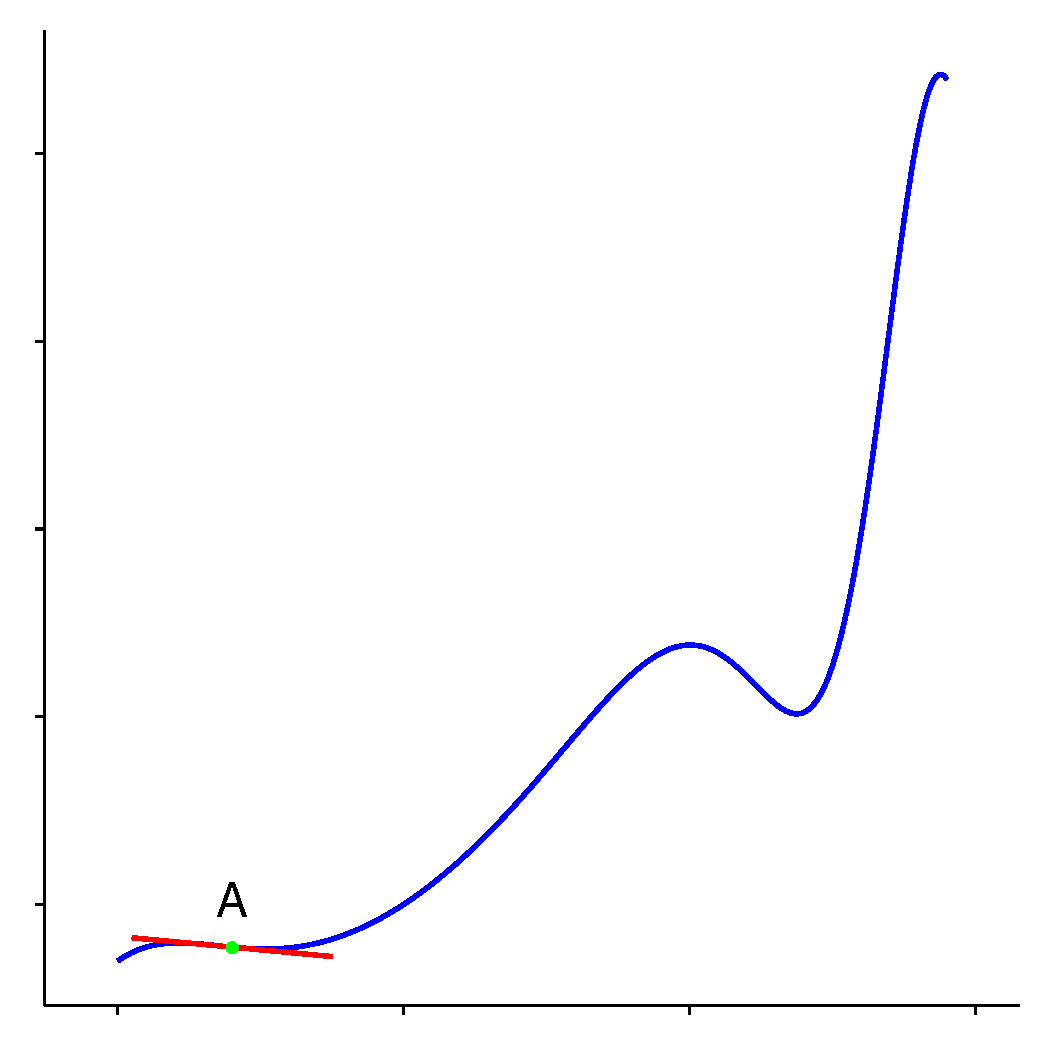
\includegraphics[width=0.65\textwidth]{der_graph1.pdf}
\end{center}
If the blue curve is a mountain, you can picture the tangeant as the slope of your skis. For example by looking at the curve in the figure on the next page, you can see that the slope of the tangent is negative in point A (when you move from left to right you go down), positive in point B (when you move from left to right you go up) and zero in point C.\\
\begin{center}
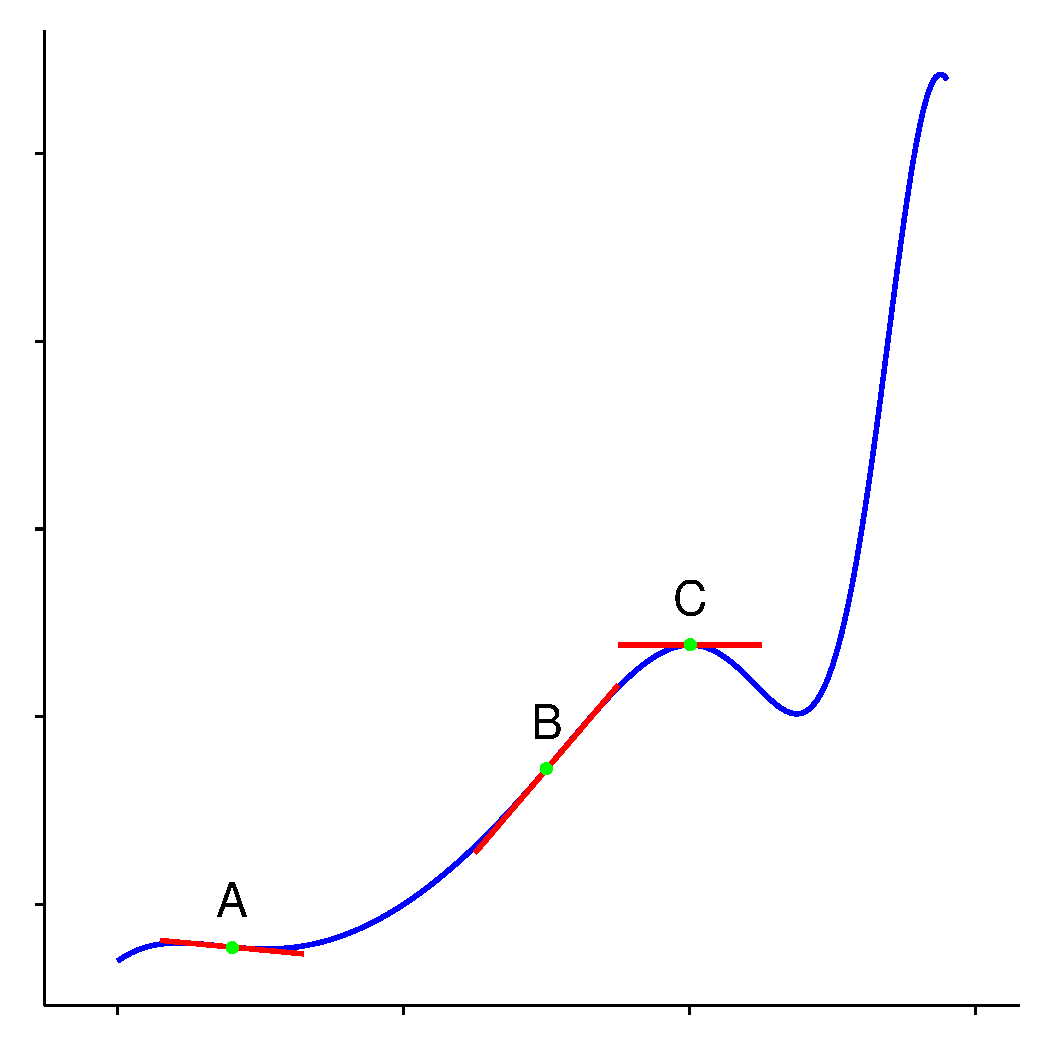
\includegraphics[width=0.65\textwidth]{der_graph2.pdf}
\end{center}
To calculate the slope of a line, we need to know two points the line goes through. This is not the case in point A as we only know one point the tangent line goes through. So we take a second point, point A\textquoteright \; below and find the slope of the line between point A and point A\textquoteright.\\ 
\begin{center}
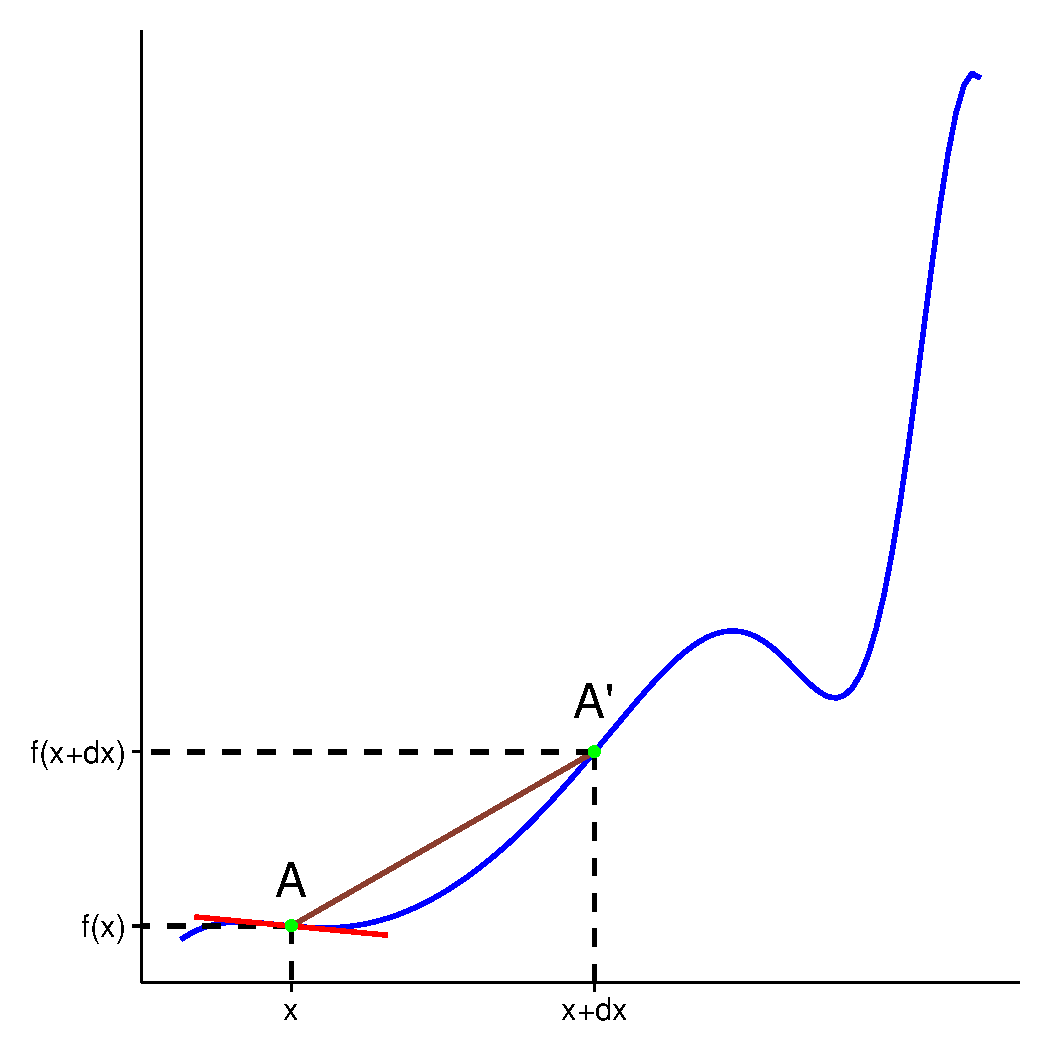
\includegraphics[width=0.8\textwidth]{der_graph3.pdf}
\end{center}
The slope is given by the rise (height) over the run (length). Let the curve be described by $y=f(x)$. The coordinate of point A is $(x, f(x))$ and the coordinate of point A\textquoteright \; is $(x+dx, f(x+dx))$. Thus the rise of the line between point A and point A\textquoteright \; is given by 
\begin{equation}
df=f(x+dx)-f(x)
\end{equation}
and the run is
\begin{equation}
dx=(x+dx)-x.
\end{equation}
So the slope is given by 
\begin{equation}
\frac{df}{dx}=\frac{f(x+dx)-f(x)}{dx}.
\end{equation}
But if you look at the graph, the slope of the line between point A and point A\textquoteright \; (brown line) is not identical to the slope of the tangent (red line). By reducing the distance between point A and A\textquoteright, which is the same as reducing $dx$, we can find lines that have slopes more similar to the tangent of point A. This is what we did in the next figure. We chose two more points, A\textquoteright\textquoteright \; and A\textquoteright \textquoteright\textquoteright \;, that are both closer to A than A\textquoteright \;. Note that the closer these points get to A\textquoteright\;, the more the line between them and A resembles the tangent of the curve in point A.\\
\begin{center}
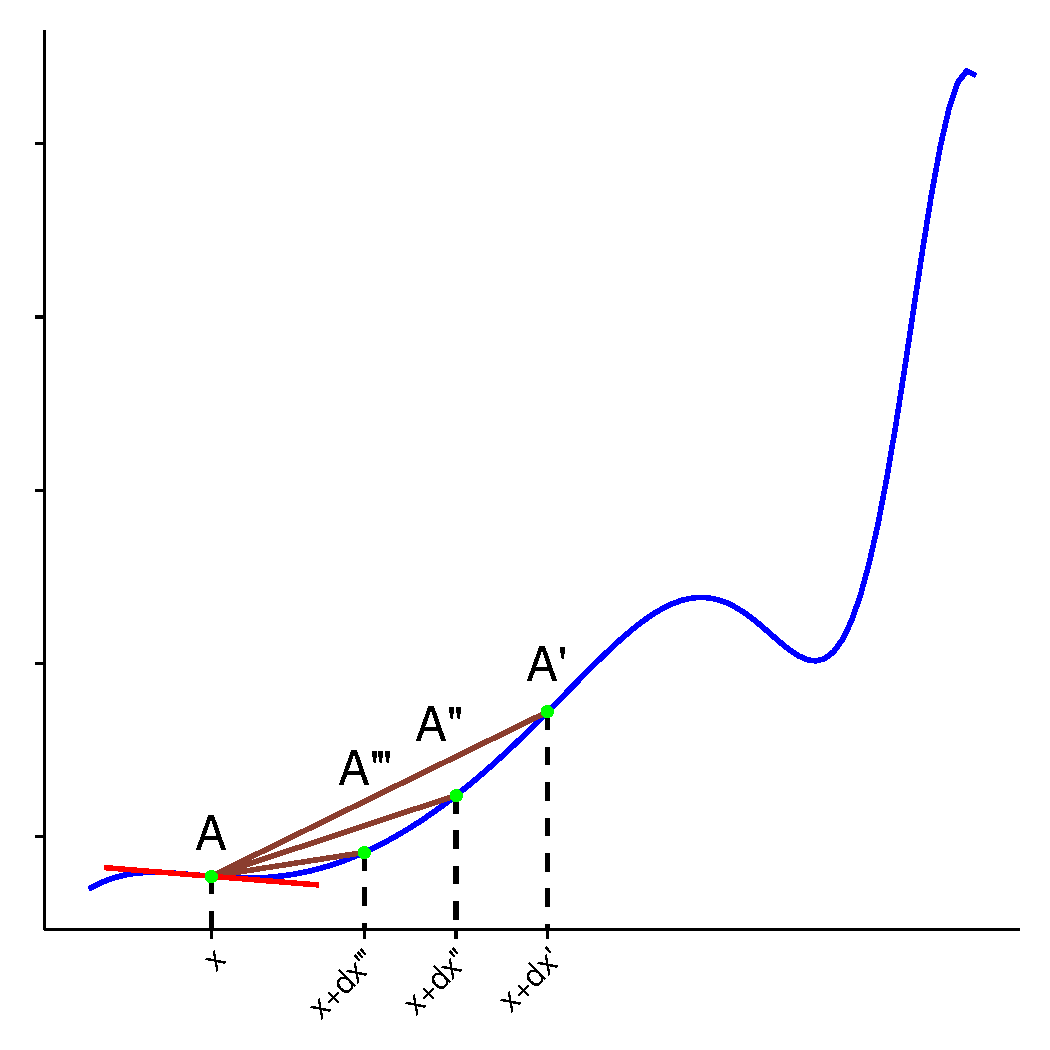
\includegraphics[width=0.85\textwidth]{der_graph4.pdf}
\end{center}
\subsection{Formal definition}
If we choose the points A and A\textquoteright \; very close together, this line will have the same slope as the tangent in point A. We thus want $dx$ to be reduced to such an extent that it tends towards zero. More precisely, we are interested in the limit when $dx$ tends towards zero:
\begin{equation}
f^\prime(x)=\lim\limits_{dx \to 0}\frac{f(x+dx)-f(x))}{dx}.
\label{eqderiv}
\end{equation}
Equation \ref{eqderiv} is the formal definition of a derivative. In this equation we used the shorthand notation for $\frac{df}{dx}$: $f^\prime (x)$.
\subsection{Interpretation of the derivative}
The first interpretation of the derivative and the only one we consider in this course is \textbf{rate of change}. The derivative describes how a function changes with respect to the independent variable x. It tells us whether the function is decreasing, increasing or remaining constant at given points. For example, in the figure below, at point A the derivative is negative (we know this from the slope of the tangent). Thus at this point the function is decreasing. Similarily, in point B the derivative is positive so the function at this point is increasing. It is important that you understand this interpretation as it is frequently used in the rest of this course to describe population growth.
\begin{center}
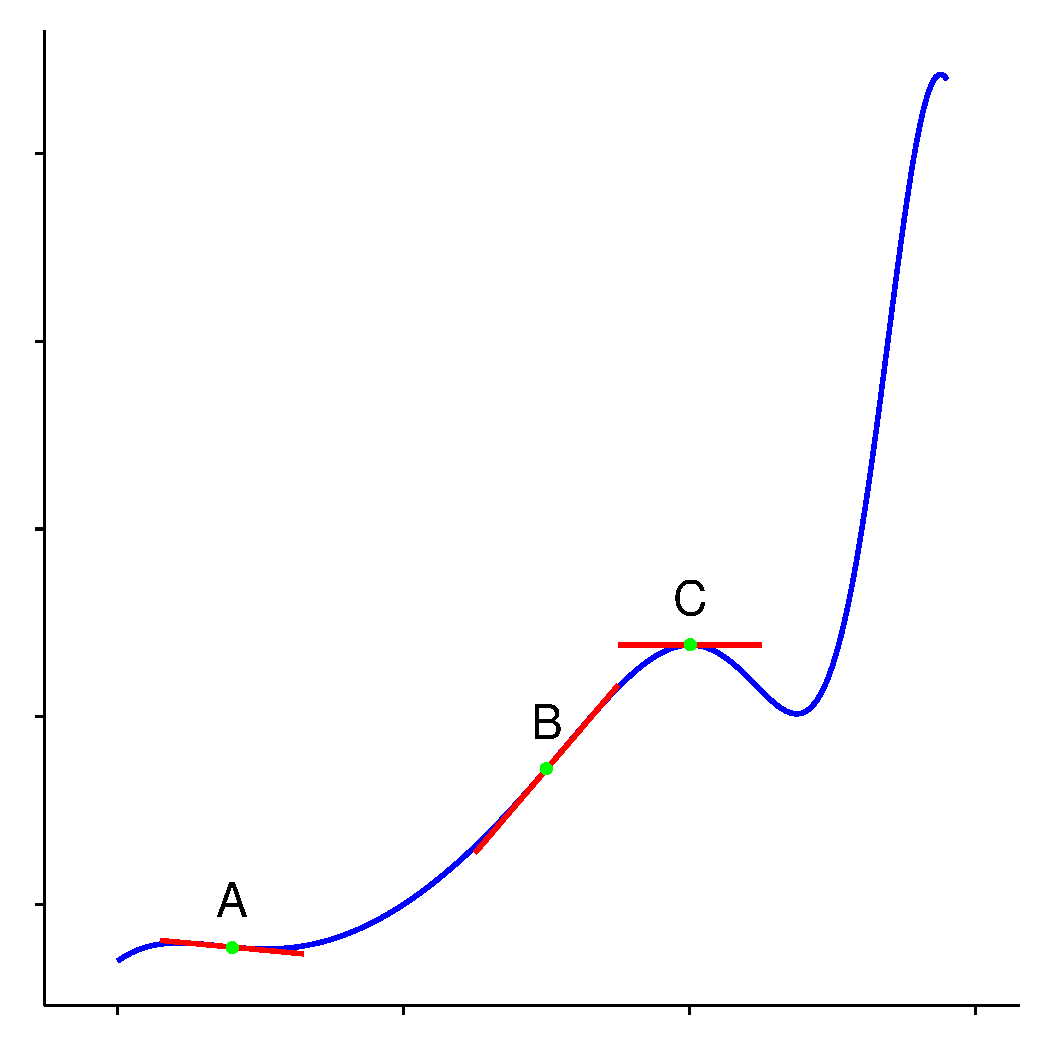
\includegraphics[width=0.55\textwidth]{der_graph2.pdf}
\end{center}
\begin{mdframed}[backgroundcolor=exampcol]
\textbf{Example}\\
\begin{center}
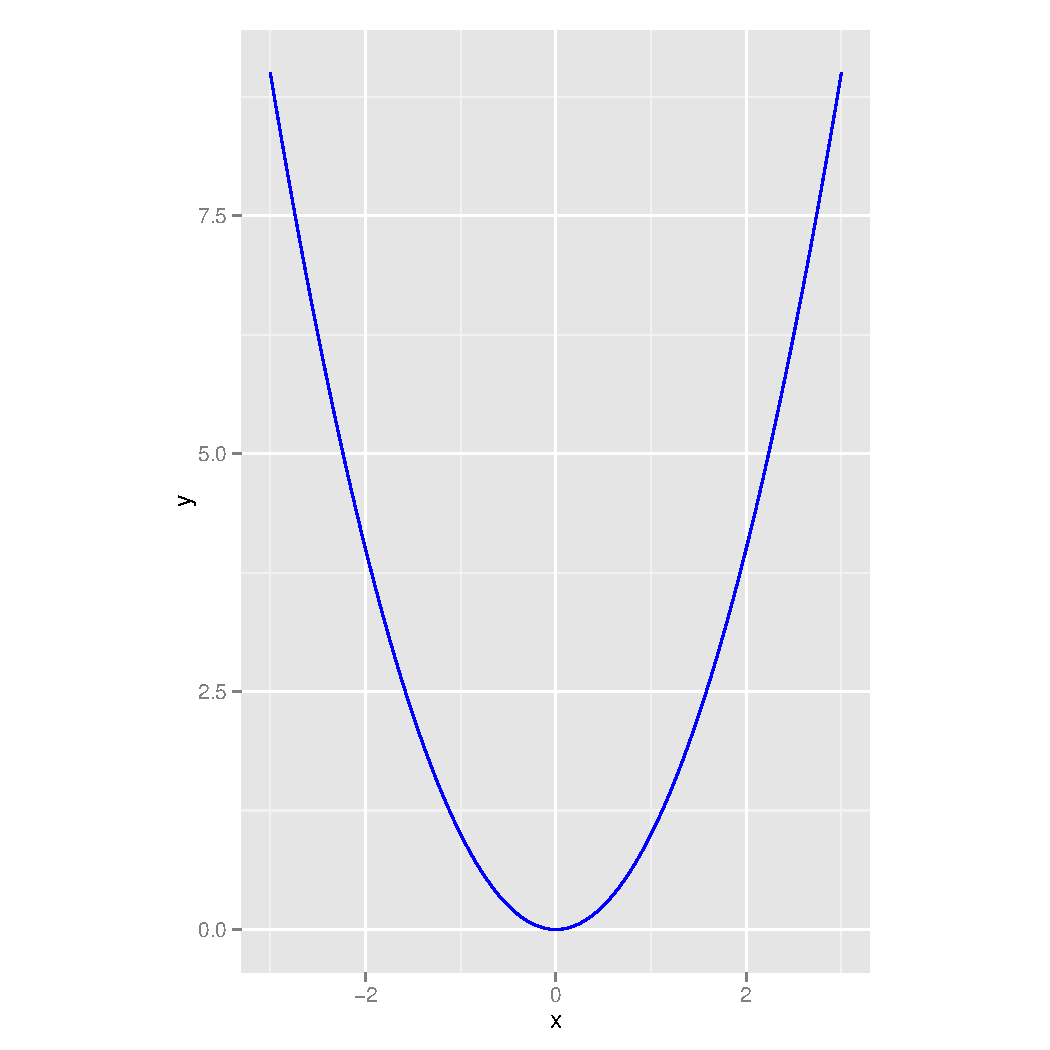
\includegraphics[width=0.65\textwidth]{der_graphquad.pdf}\\
\end{center}
As an example, let us work out the derivative of a simple quadratic function. The function of the curve in the figure is given by: 
\begin{equation}
f(x)=x^2.
\label{eqquad}
\end{equation}
The derivative is given by the formal definition of the derivative (see previous section, equation \ref{eqderiv}) and by substituting $f(x)$ by equation \ref{eqquad}, we find:
\begin{equation}
f^\prime(x)=\lim\limits_{dx \to 0}\frac{(x+dx)^2-x^2}{dx}.
\end{equation}
When we multiply the brackets out, we are left with: 
\begin{equation}
f^\prime(x)=\lim\limits_{dx \to 0}\frac{x^2+2xdx+dx^2-x^2}{dx}
\end{equation}
By simplification we get:
\begin{equation} 
f^\prime(x)=\lim\limits_{dx \to 0}2x+dx
\end{equation}
But when $dx$ tends towards zero we are only left with:
\begin{equation}
f^\prime(x)=2x
\end{equation}
This mean that the instantenous rate of change of any point on the curve is $2x$. Or in other words: the derivative of $x^2$ with respect to $x$ is $2x$. For instance, the slope of the tangent in $x=4$ is $2 \cdot 4=8$. Thus the instantenous rate of change in $x=4$ is $8$.
\end{mdframed}

\subsection{General rule}
We do not demonstrate this here but in general the following holds:
\begin{align}
f(x)=x^n & &\rightarrow & &f^\prime(x)=nx^{n-1}
\end{align}
When a function is the sum of two functions (for example $h(x)$ and $u(x)$), its derivative is the sum of the derivatives of these two functions, thus:
\begin{align}
f(x)=u(x)+h(x)& &\rightarrow & & f^\prime(x)=u^\prime(x)+h^\prime(x)
\end{align}
When a function is multiplied by a constant, for example $c$, then the derivative is the derivative of the function multiplied by the constant.
\begin{align}
f(x)=c\cdot u^\prime(x)& &\rightarrow & & f^\prime(x)=c\cdot u^\prime(x)
\end{align}

%%%%%%% CHAIN RULE %%%%%%%%%%%%%%%%%%%%%%%%%%%%%%%%%%%
\subsection{Chain rule}
The general rule presented in the previous section is nice, but not very helpful when we move to more complicated formulas. What happens for example if functions become nested, what if for example a function $h$ depends on $u$ and $u$ in turn depends on $x$. How does $f$ now change if $x$ changes? We are thus faced with the following function:
\begin{equation}
f(x) = h(u(x))
\end{equation}
Formally the chain rule states
\begin{equation}
f^\prime(x)=h^\prime(u) u^\prime(x) = \frac{df}{du}\frac{du}{dx}
\end{equation}


\begin{mdframed}[backgroundcolor=exampcol]
\textbf{Example}\\
So far it is all a bit vague, we agree on that, so let's move to an example:
\begin{equation}
f(x)=(x^2-4)^5
\label{eqexder}
\end{equation}
Equation \ref{eqexder} can be decomposed in two functions; an "outer" function and an "inner" function. The outer function is raising to the power $5$. The inner function is the content of the brackets. Let us call the inner function of $f(x)$, $u(x)$. 
\begin{equation}
u(x)=(x^2-4)
\label{yuk0}
\end{equation}
Let us call the outer function $h(u)$
\begin{equation}
h(u)=u^5
\end{equation}
With the chain rule
\begin{equation}
f^\prime(x)=h^\prime(u)\cdot u^\prime(x)
\label{yuk3}
\end{equation}
\begin{equation}
h^\prime(u)=5u^4
\label{yuk1}
\end{equation}
\begin{equation}
u^\prime(x)=2x
\label{yuk2}
\end{equation}
We have now calculated all the separate terms in equation \ref{yuk3}, all we need to do is fill in equations \ref{yuk1}, \ref{yuk2} and \ref{yuk0} to obtain our final answer:
\begin{equation}
f^\prime(x)=5(x^2-4)^4 2x.
\end{equation}
\end{mdframed}

%%%%%%% PROD RULE %%%%%%%%%%%%%%%%%%%%%%%%%%%%%%%%%%%
\subsection{Product rule}
Another useful rule to find the derivative of a function is the product rule. The product rule is used to find the derivative of the multiplication of two functions. Formally the product rule is 
\begin{equation}
(h(x)\cdot g(x))^\prime=h^\prime(x)\cdot g(x)+h(x)\cdot g^\prime(x)
\end{equation}


\begin{mdframed}[backgroundcolor=exampcol]
\textbf{Example}\\
Let us work out as an example the derivative of the following function: 
\begin{equation}
f(x)=5x(x^2-3)
\end{equation}
$f(x)$ is composed of two functions; Let
\begin{equation}
f(x) = h(x)\cdot g(x)
\end{equation}
with
\begin{equation}
h(x)=5x
\end{equation}
and 
\begin{equation}
g(x)=x^2-3
\end{equation}
The product rule states
\begin{equation}
f^\prime(x)=h^\prime(x)g(x)+h(x)g^\prime(x)
\label{eqprodex}
\end{equation}
The derivatives of the functions $h(x)$ and $g(x)$ are:
\begin{equation}
h^\prime(x)=5
\end{equation}
\begin{equation}
g^\prime(x)=2x
\end{equation}
We now have all the information to fill in equation \ref{eqprodex}, by doing so we find:
\begin{equation}
\begin{aligned}
f^\prime(x)&=&5(x^2-3)+(5x)\cdot (2x)\\
&=&5x^2-15+10x^2\\
&=&15(x^2-1)
\end{aligned}
\end{equation}
\end{mdframed}

%%%%%%% EXERCISES %%%%%%%%%%%%%%%%%%%%%%%%%%%%%%%%%%%
\subsection{Exercises}
$\;$
\begin{Exercise}[title= Answer the following questions by looking at the graphs,label=ex0,difficulty=1]
\newcommand{\rat}{0.65}
\newcommand{\rati}{0.35}


\begin{minipage}{\rat\textwidth}
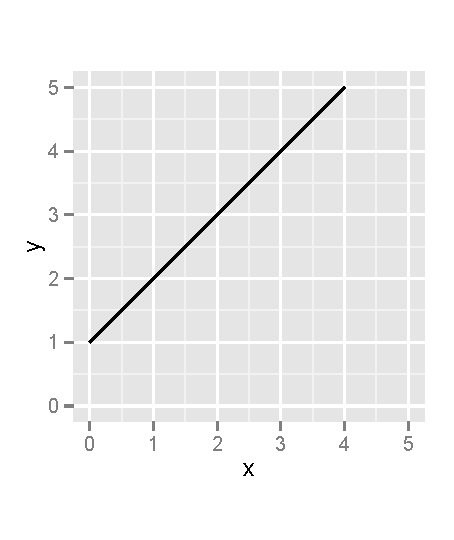
\includegraphics[width=0.75\textwidth]{1a.pdf}
\end{minipage}
\begin{minipage}{\rati\textwidth}
1. By looking at the graph, give the derivative of the function. Bonus question: Find the equation from the graph.
\end{minipage}

\begin{minipage}{\rat\textwidth}
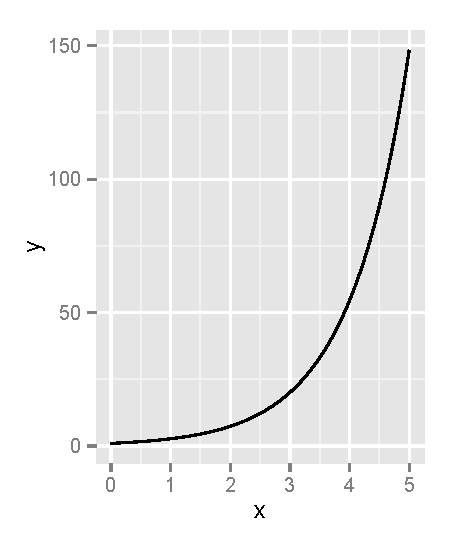
\includegraphics[width=0.75\textwidth]{1b.pdf}
\end{minipage}
\begin{minipage}{\rati\textwidth}
2. Show in the graph the part where the derivative is larger than $0$. Bonus question: Find the equation from the graph.
\end{minipage}

\begin{minipage}{\rat\textwidth}
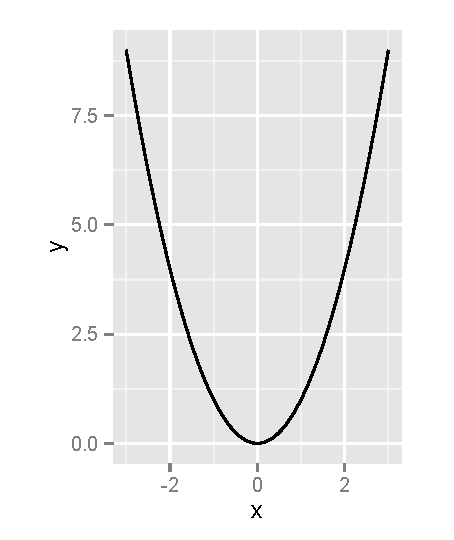
\includegraphics[width=0.75\textwidth]{1c.pdf}
\end{minipage}
\begin{minipage}{\rati\textwidth}
3. Show in the graph where the point where the derivative is $0$. At point ($2$,$4$) is the derivative smaller, larger or equal to $0$? Same question for point ($-2$, $4$). Bonus question: Find the equation from the graph. 
\end{minipage}

\begin{minipage}{\rat\textwidth}
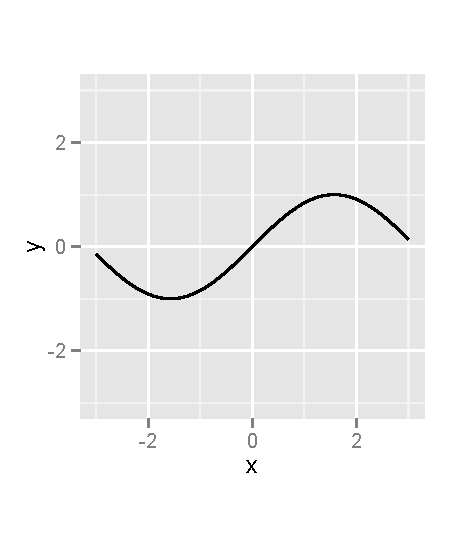
\includegraphics[width=0.75\textwidth]{1d.pdf}
\end{minipage}
\begin{minipage}{\rati\textwidth}
4. Show in the graph where the derivative is $0$. Give the derivative of the point ($0$,$0$). Bonus question: Find the equation from the graph.
\end{minipage}

\begin{minipage}{\rat\textwidth}
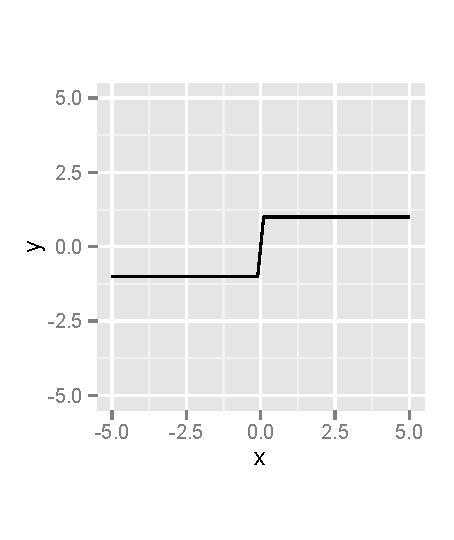
\includegraphics[width=0.75\textwidth]{1e.pdf}
\end{minipage}
\begin{minipage}{\rati\textwidth}
5. Give the derivatives at ($-5$, $-1$) and ($3$,$1$).
\end{minipage}


\begin{minipage}{\rat\textwidth}
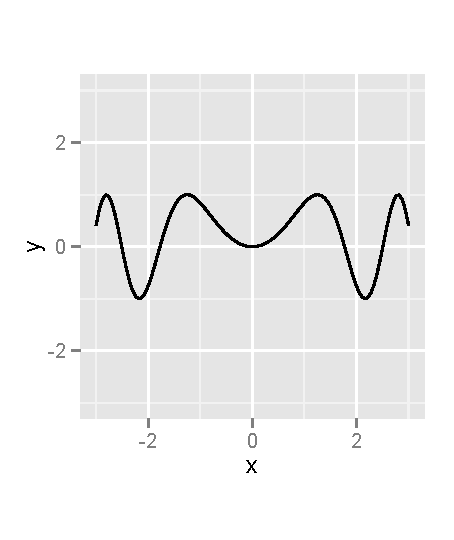
\includegraphics[width=0.75\textwidth]{1f.pdf}
\end{minipage}
\begin{minipage}{\rati\textwidth}
6. Show in the graph the points where the derivative is $0$. How many points are they? Show in the graph the parts where the derivative is smaller than $0$.
\end{minipage}
\end{Exercise}
\begin{Answer}[ref=ex0]
\newcommand{\rat}{0.55}
\newcommand{\rati}{0.45}

\begin{minipage}{\rat\textwidth}
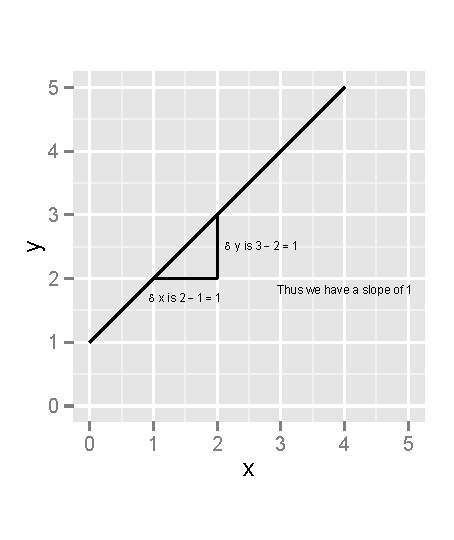
\includegraphics[width=0.85\textwidth]{1aa.pdf}
\end{minipage}
\begin{minipage}{\rati\textwidth}
1. The linear function below has a slope of $1$; if you increase the $x$ value by one unit, you increase the $y$ value by one unit. Remember that the slope of the tangent line is equal to the derivative of a curve. For linear functions, the tangent is the very same function. Thus, the derivative of this function is $1$, the slope of the tangent. Bonus question: This function has an intercept of $1$ (where the line crosses the y axis): $f(x)=x+1$.
\end{minipage}

\begin{minipage}{\rat\textwidth}
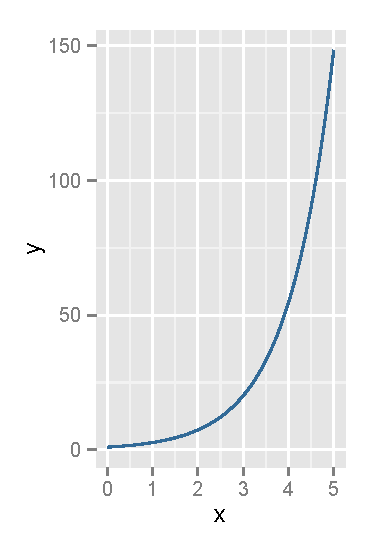
\includegraphics[width=0.85\textwidth]{1ab.pdf}
\end{minipage}
\begin{minipage}{\rati\textwidth}
2. The tangents in every point of the graph depicted below (except at ($0$,$0$)) have a positive slope. In other word, a derivative greater than zero. Bonus question: This function is exponential: $f(x)=e^x$
\end{minipage}

\begin{minipage}{\rat\textwidth}
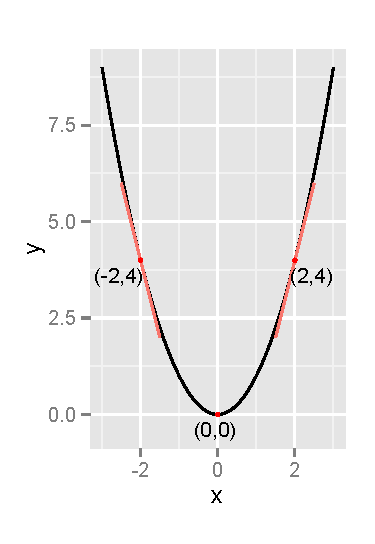
\includegraphics[width=0.85\textwidth]{1ac.pdf}
\end{minipage}
\begin{minipage}{\rati\textwidth}
3. The derivative is $0$ in ($0$,$0$). At ($2$,$4$), the derivative is greater than zero, as you can see on the graph, the slope of the tangent is positive. In contrast, at ($-2$,$4$), the derivative is smaller than $0$. The slope of the tangent is negative. Bonus question: This is a quadractic function: $f(x)=x^2$. 
\end{minipage}

\begin{minipage}{\rat\textwidth}
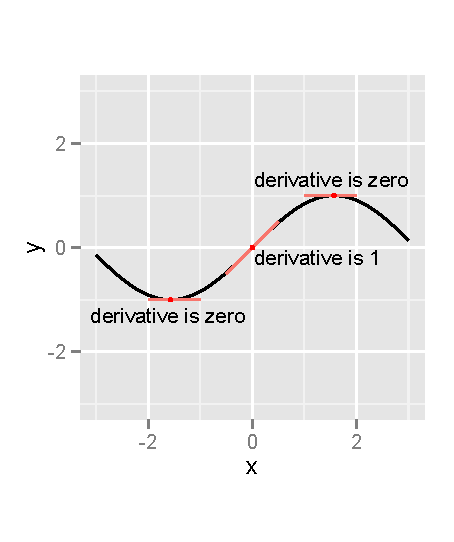
\includegraphics[width=0.85\textwidth]{1ae.pdf}
\end{minipage}
\begin{minipage}{\rati\textwidth}
4. The derivative is $0$ at the minimum and maximum, where the slope of the tangent is $0$. At point ($0$,$0$) the derivative is $1$, which you can find from the slope of the tangent by reading the graph. Bonus question: This is a trigonometic function: $f(x)=sin(x)$.
\end{minipage}

\begin{minipage}{\rat\textwidth}
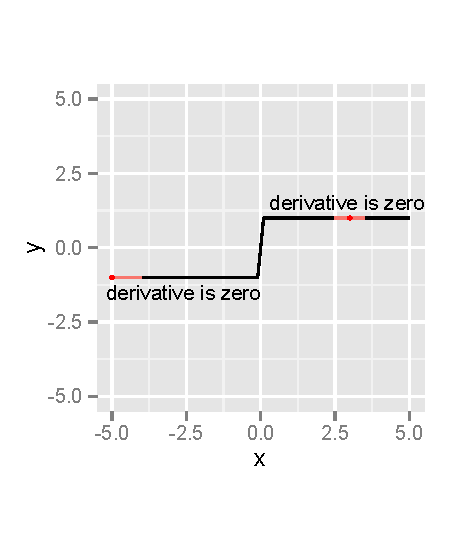
\includegraphics[width=0.85\textwidth]{1af.pdf}
\end{minipage}
\begin{minipage}{\rati\textwidth}
5. The derivatives at (-5, -1) and (3,1) are zero. See the slope of the tangent line at those points.
\end{minipage}


\begin{minipage}{\rat\textwidth}
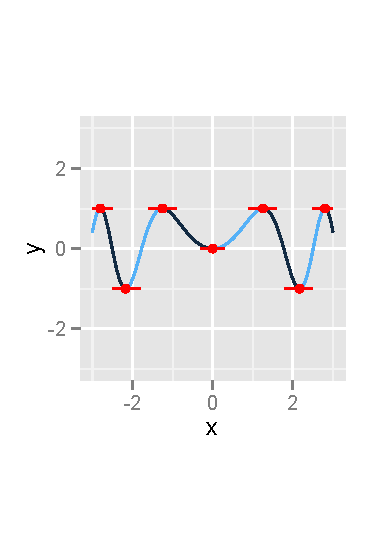
\includegraphics[width=0.85\textwidth]{1ag.pdf}
\end{minipage}
\begin{minipage}{\rati\textwidth}
6. This trigonometric functions has 7 minimums and maximums, each with a derivative of $0$. They are indicated in the graphy by the large dots. The parts of the graph with negative derivatives are shown in dark blue. In those part, the slope of the tangent is always smaller than $0$.
\end{minipage}
\end{Answer}

\begin{Exercise}[title=Find the derivatives of the following functions,label=ex1,difficulty=1]
\begin{align*}
a(x) &= -12  		&  e(x) &= (x-3)^2 \\
b(x) &= x^2 		&  f(x) &= (-2x-1)^6\\
c(x) &= 5x^3 + 2 	&  g(x) &= \frac{x^2-1}{6x^4} \\
d(x) &= \frac{5}{2}x^2-3x &  h(x) &= \frac{(x^2-2)^2}{x^2}
\end{align*}
\end{Exercise}
\begin{Answer}[ref=ex1]
\noindent The first function is easy: the function is a constant (it is always $-12$), so the slope of the function is $0$:
\begin{equation*}
a^\prime (x) = 0
\end{equation*}
The next three derivatives are also relatively straightforward, they are combinations of the standard derivatives:
\begin{align*}
b^\prime (x) &= 2 x & c^\prime (x) &= 15x^2 & d^\prime (x) &= 5x-3
\end{align*}
The next two derivatives require the chain rule:
\begin{equation*}
e(x) = (x-3)^2
\end{equation*}
if $u(x)=(x-3)$, we can write:
\begin{align*}
e(u)&=u^2  & \rightarrow & &e^\prime(x)&=e^\prime(u)u^\prime(x)=2u(x)\cdot u^\prime(x).
\end{align*}
The next step is finding the derivative of $u(x)$:
\begin{equation*} 
u^\prime(x)=1
\end{equation*}
Finally we use this to find $e^\prime(x)$:
\begin{equation*}
e^\prime(x)=2\cdot (x-3)\cdot 1 =2x-6.
\end{equation*}\\

\begin{equation*}
f(x) = (-2x-1)^6
\end{equation*}
We set $u(x)=(-2x-1)$ to find:
\begin{align*}
f(x)&=u^6 & \rightarrow & & f^\prime(x)&=6u(x)^5\cdot u^\prime(x)
\end{align*}
Now we find $u^\prime(x)$:
\begin{equation*} 
u^\prime(x)=-2
\end{equation*}
Now all that is left is putting $u(x)$ and $u^\prime$ in the expression for $f^\prime(x)$: 
\begin{equation*}
f^\prime(x)=6\cdot(-2x-1)^5\cdot(-2)=-12(-2x-1)^5
\end{equation*}

\noindent The next derivative can be solved in multiple ways. Here we show how to solve it with the product rule. First we rearrange the equation.
\begin{equation*}
g(x) = \frac{x^2-1}{6x^4} =  \frac{1}{6} \cdot x^{-4} \cdot (x^2-1) \\
\end{equation*}
Now that we have only multiplications, we can use the product rule, first we set:
\begin{align*}
g(x)&=u(x)v(x) & u(x)&= x^2-1 & v(x)&= \frac{1}{6}\cdot x^{-4}
\end{align*}
Now we know from the product rule that:
\begin{equation*}
g^\prime(x) = u(x)v^\prime(x) + u^\prime(x)v(x)
\end{equation*}
Next is finding $u^\prime(x)$ and $v^\prime(x)$, luckily this is not too complicated:
\begin{align*}
u^\prime(x) &= 2x & v^\prime(x) &= -\frac{4}{6}x^{-5}
\end{align*}
Now we have everything to find $g^\prime(x)$:
\begin{align*}
g^\prime(x) & = -\frac{4}{6} x^{-5} \cdot (x^2-1) + \frac{2}{6} x \cdot x^{-4} \\
& = \frac{1}{6} (-4x^{-3} +4x^{-5} +2x^{-3}) \\
& = \frac{1}{3} (-x^{-3} +2x^{-5}) \\
& = \frac{-x^2+2}{3x^5}
\end{align*}
\begin{mdframed}
\textit{But I don't like the product rule... (for emotional/personal reasons)}\\
In this case that's fine, just realise that:
\begin{equation*}
g(x) = \frac{x^2-1}{6x^4} = \frac{x^2}{6x^4} - \frac{1}{6x^4} = \frac{1}{6} x^{-2} - \frac{1}{6}x^{-4}.
\end{equation*}
And then we see:
\begin{equation*}
g^\prime(x) = -\frac{2}{6}x^{-3} + \frac{4}{6} x^{-5} = \frac{1}{3} (-x^{-3} + 2x^{-5}) = \frac{-x^2+2}{3x^5}.
\end{equation*}
Fortunately the answer is without product rule the same...
\end{mdframed}
Similar to the previous one, the last function can be solved in different ways, but this time the product rule is probably the simpler one (but feel free to try other ways of course):
\begin{equation*}
h(x) = \frac{(x^2-2)^2}{x^2} = (x^2-2)^2 \cdot x^{-2} \\
\end{equation*}
\begin{align*}
h(x) &= u(x) v(x) & u(x) &=(x^2-2)^2 & v(x) &=x^{-2} 
\end{align*}
Now according the product rule:
\begin{equation*}
h^\prime(x) = u^\prime(x) v(x) + u(x) v^\prime(x)
\end{equation*}
First we will look for $u^\prime(x)$. For this we need to use the chain rule (yes that is quite something... using the chain rule inside of the product rule...). To do so, we write:
\begin{align*}
u(w) &= w^2 & w(x)&=x^2-2
\end{align*}
Now we now that
\begin{equation*}
u^\prime(x)= u^\prime(w)\cdot w^\prime(x) = 2w\cdot w^\prime(x)
\end{equation*}
We first find $w^\prime(x)$:
\begin{equation*}
w^\prime(x)=2x.
\end{equation*}
And thus:
\begin{equation*}
u^\prime(x)=2(x^2-2)\cdot 2x =4x^3 -8x.
\end{equation*}
The next ingredient for finding $h(x)$ is $v^\prime(x)$, since $v(x)=x^{-2}$, we find:
\begin{equation*}
v^\prime(x) = -2x^{-3}
\end{equation*}
Finally we found all the ingredients that we needed for $h^\prime(x)$, so lets add everything together and solve the exercise:
\begin{equation*}
 h^\prime(x) = (4x^3-8x) \cdot x^{-2} + (x^2-2)^2 \cdot-2x^{-3}  = \frac{4 \cdot (x^2-2)} {x}-\frac{2\cdot (x^2-2)^2}{x^3}
\end{equation*}
\end{Answer}


\begin{Exercise}[title= (Optional) Find the derivatives of the following functions,difficulty=3,label=ex2]
\begin{eqnarray*}
a(x) & = & sin(x^2+x)\\
b(x) & = & cos(x+3)
\end{eqnarray*}
\textit{Hint: \\if $f(x)=sin(x)$, then $f^\prime(x)=cos(x)$ \\if $f(x)=cos(x)$, then $f^\prime(x)=-sin(x)$.}
\end{Exercise}
\begin{Answer}[ref=ex2]
\noindent In addition to the special derivatives of the trigonometric functions, you need to apply the chain rule. 
\begin{equation*}
a(x)=sin(x^2+x)
\end{equation*}
Now we write:
\begin{align*}
a(u) &= sin(u) & u(x)&=x^2+x
\end{align*}
Now it has to hold that (if you believe in the chain rule):
\begin{equation*}
a^\prime(x) = a^\prime(u) u^\prime(x)
\end{equation*}
We know that:
\begin{align*}
a^\prime(u) &= cos(u) & u^\prime(x)&=2x+1
\end{align*}
So we solve the exercise without too much headache:
\begin{equation*}
a^\prime(x)= cos(u) \cdot u^\prime(x) = (2x+1)\cdot cos(x^2+x) 
\end{equation*}\\
\\
The procedure is just... the same:
\begin{equation*}
b(x)=cos(x+3)
\end{equation*}
\begin{align*}
b(u)&=cos(u) & u(x)&=x+3 & b^\prime(x) = b^\prime(u) u^\prime(x).
\end{align*}
We find the derivatives:
\begin{align*}
b^\prime(u) &= -sin(u) & u^\prime(x) &= 1
\end{align*}
We fill this in:
\begin{equation*} 
b^\prime(x) = -sin(x+3) \cdot 1= -sin(x+3) 
 \end{equation*}
And finally (at least while writing this we were slow, maybe you were fast instead), we finish the last exercise concerning derivatives!

\end{Answer}
%%%%%%% INTEGRATION %%%%%%%%%%%%%%%%%%%%%%%%%%%%%%%%%%%
\section{Integrals}
\subsection{Graphical definition}
Graphically, an integral is \textbf{the area below a curve.} The shaded area in the figure below is the integral of the blue curve between $x=a$ and $x=b$.\\
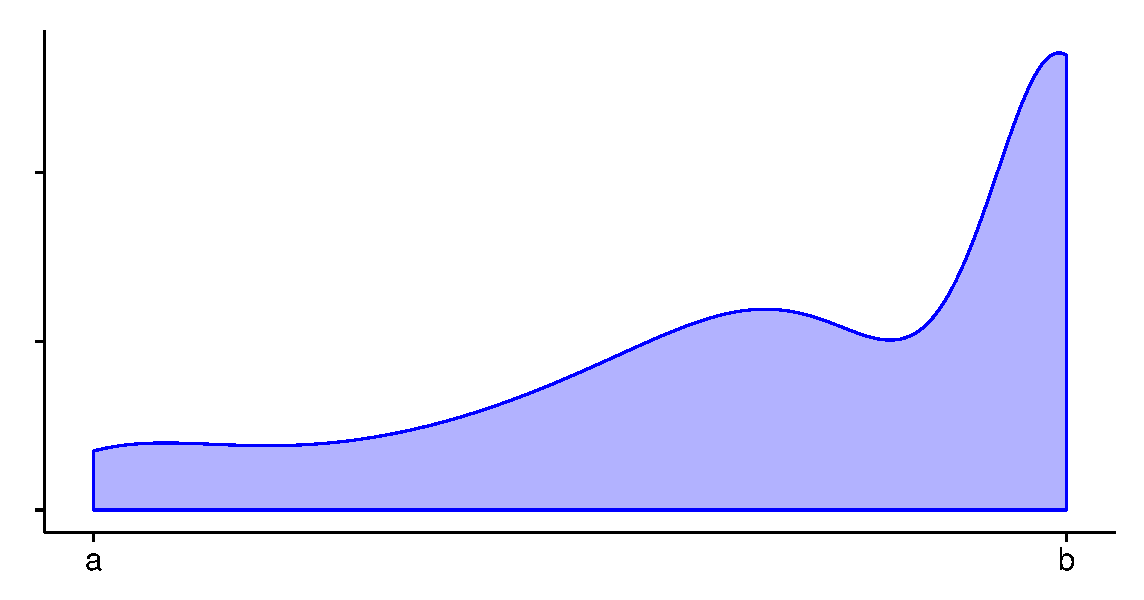
\includegraphics[width=0.85\textwidth,height=0.6\textwidth]{int_graph1.pdf}\\
An approximation of the shaded area can be obtained by dividing the area in small rectangles. This is interesting because calculating the area of a rectangle is simple: it is the width times the height. This is what is illustrated in the figure below. The $x-$axis has been divided in multiple segments of identical width $dx$.\\
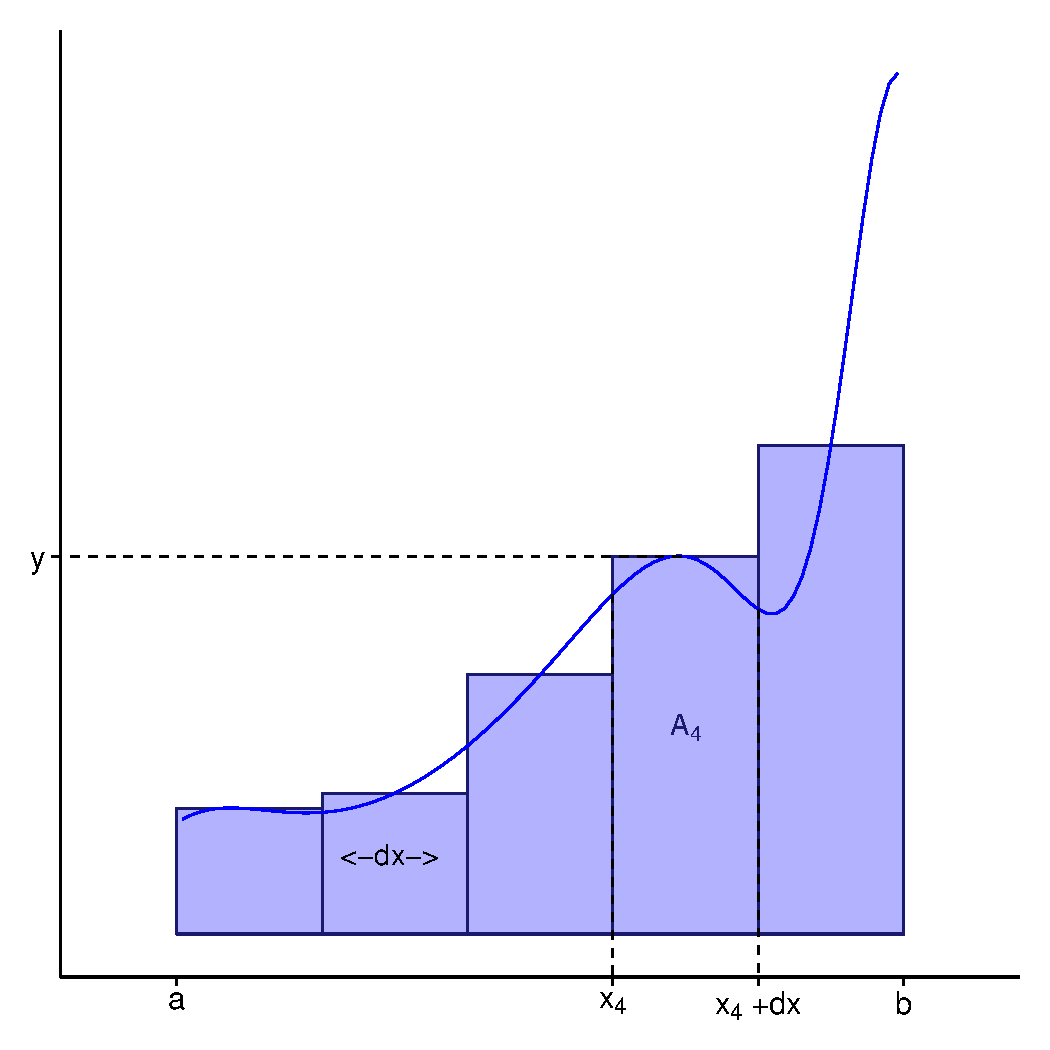
\includegraphics[width=0.85\textwidth]{int_graph2.pdf}\\
Let us look more closely at the fourth rectangle ($A_4$). This rectangle lies between $x_4$ and $x_4+dx$. The height of the rectangle is equal to the height of the curve at the mid-point between $x_4$ and $x_4+dx$. We will call this point  $x_4^*$ (and thus $x_4^* = x_4 + \frac{1}{2} dx$).  Let $f(x)$ be the function of the curve. The area of the rectangle, $A_4$, is $f(x_i^*)$, the height times $dx$, the width. 
\begin{equation}
A_{4}=f(x_{4}^*)dx
\end{equation}
We can repeat this for all rectangles in the figure. The total area under the curve ($A$) can then be approximated by the sum of all rectangles. 
\begin{equation}
A \approx A_1 + A_2 + A_3 + A_4 +A_5
\end{equation}
Now we have divided the $x-$axis between $a$ and $b$ in five bins. If instead we divide it in $n$ bins, we get the following expression:
\begin{equation}
\begin{aligned}
A&\approx A_{1}+A_{2}+ ...A_{n}\\
&= f(x_{1}^*)dx+f(x_{2}^*)dx+...+f(x_{n}^*)dx\\
&= \sum\limits_{i=1}^nf(x_{i}^*)dx
\end{aligned}
\end{equation}
\begin{center}
\newcommand{\blub}{0.45\textwidth}
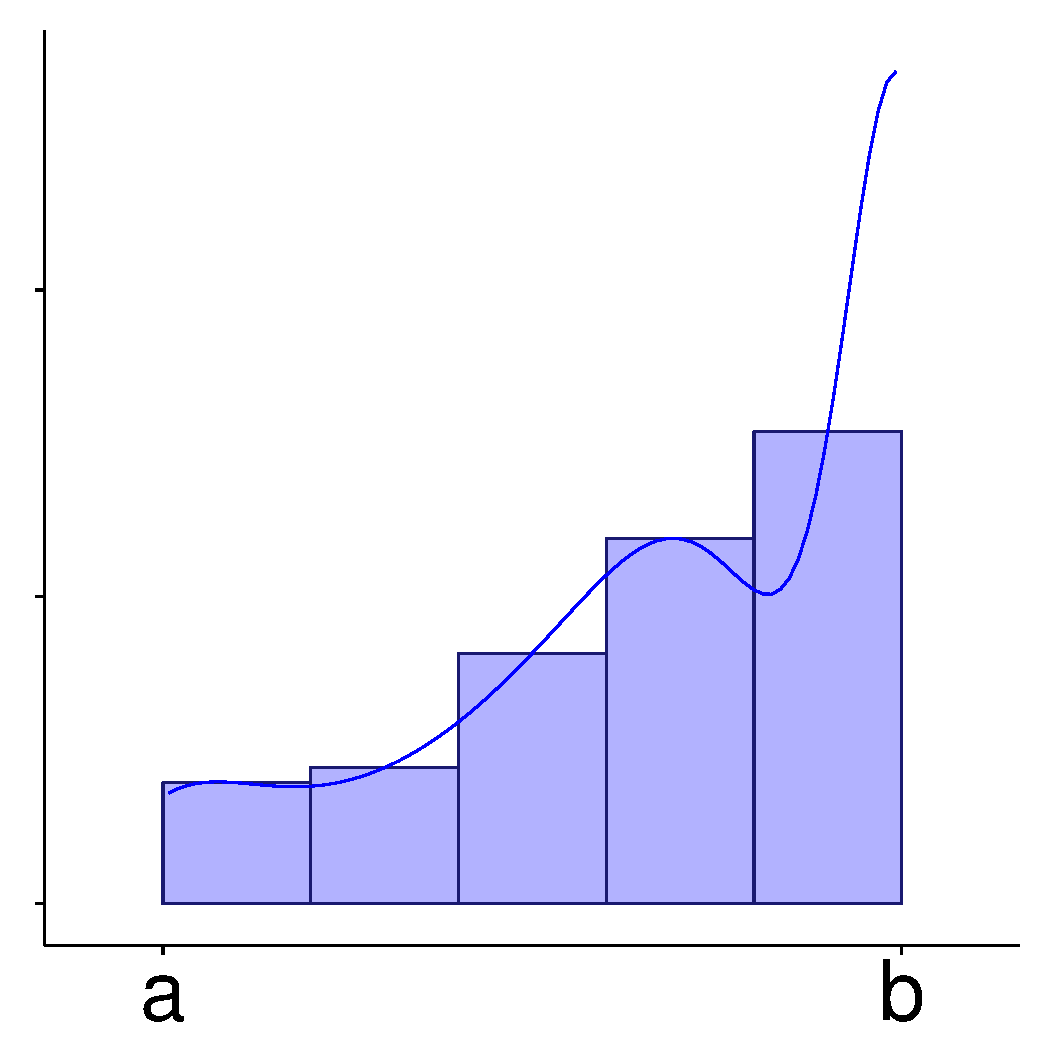
\includegraphics[width=\blub,page=1]{int_graph3.pdf}
\includegraphics[width=\blub,page=2]{int_graph3.pdf}\\
\includegraphics[width=\blub,page=3]{int_graph3.pdf}
\includegraphics[width=\blub,page=4]{int_graph3.pdf}\\
\end{center}
The smaller the interval is, the closer the approximated area will be to the actual area. To state this differently: the larger the number of intervals ($n$), the better the approximation. 
\begin{mdframed}
There is of course a relationship between the number of intervals ($n$) and the size of each interval ($dx$). If we integrate from $x=a$ to $x=b$, the length ($L$) of this range is:
\begin{equation*}
L = b - a
\end{equation*}
If we divide this length in $n$ bins with equal size $dx$, this size will be:
\begin{equation*}
dx = \frac{L}{n}
\end{equation*}
\end{mdframed}


%%%%%%%%% FORMAL DEFINITION %%%%%%%%%%%%%%%%%%%%%%
\subsection{Formal definition}
We want the number of intervals $n$ to approach infinity. In other words we are interested in the case where the limit of $n$ tends towards infinity: this is when the approximaiton is the true area under the curve.
\begin{equation}
A=\lim\limits_{n \to \infty}\sum\limits_{i=1}^nf(x_{i}^*)dx
\end{equation}
Formally an integral is defined as:
\begin{equation}
\int f(x)dx=\lim\limits_{n \to \infty}\sum\limits_{i=1}^nf(x_{i}^*)dx
\end{equation}
An integral is in a sense \textbf{the reverse of a derivative}. Given a function $f(x)$, the primitive of this function is any function $F(x)$ such that
\begin{equation}
F^\prime(x)=f(x)
\end{equation}
The integral of $f(x)$ over the interval $\left[a,b\right]$:
\begin{equation}
\int_{x=a}^b f(x)dx=F(b)-F(a)
\end{equation}


\begin{mdframed}[backgroundcolor=exampcol]
\textbf{Example}\\
We will now illustrate this by calculating the area of the curve $f(x)=x$ between $x=a$ and $x=b$.\\
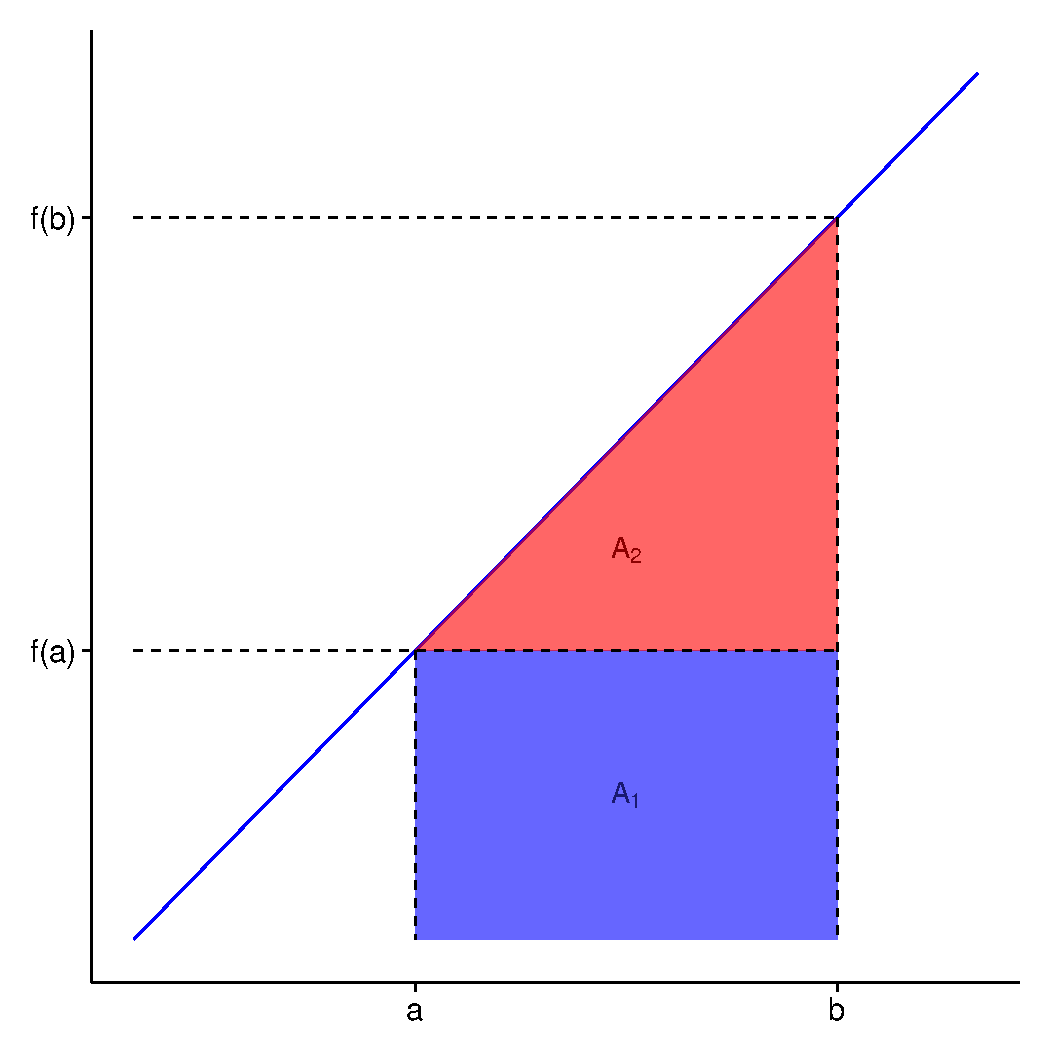
\includegraphics[width=0.75\textwidth]{int_graph4.pdf}\\
Because $f(x)=x$, $f(a)=a$ and $f(b)=b$.\\[0.5ex]
\noindent\textit{Graphically}\\
We can divide the area that we are interested in into two smaller areas: a rectangle ($A_1$) and a triangle ($A_2$). For both of these it is easy to calculate the area.

First we calculate the area of the rectangle ($A_1$), for this we multiply its width ($b-a$) by its height ($f(a) = a$):
\begin{equation*}
A_1 = (b-a)a = ba - a^2
\end{equation*}
Next we calculate the area of the rectangle ($A_2$). This is equal to one half times its width ($b-a$) times its height ($f(b)-f(a)=b-a$):
\begin{equation*}
A_2 = \frac{1}{2} (b-a)(b-a) = \frac{1}{2} \left(b^2 + a^2 - 2ba \right) = \frac{1}{2} b^2 + \frac{1}{2} a^2 - ba 
\end{equation*}
We find the the total area under the curve by adding up the areas of the rectangle and the triangle:
\begin{equation*}
A = A_1 + A_2 = \frac{1}{2} b^2 - \frac{1}{2} a^2.
\end{equation*}\\[0.5ex]
\noindent\textit{Numerically}\\
We are looking for a function $F(x)$, such that $F^\prime(x) = f(x)$. In words, we are looking for a function which derivative is $x$, because a primitive is the reverse function of a derivative. Remember that the derivative of $x^2$ is $2x$, so $x^2$ is close to the function we are looking for. In fact, it is $2$ times too high. So why not just divide it by $2$?
\begin{equation*}
F(x) = \frac{1}{2} x^2.
\end{equation*}
But is $\frac{1}{2} x^2$ really the derivative of $x$? Let us check by applying the general rule of derivatives: 
\begin{eqnarray*}
F^\prime(x) &=& \frac{1}{2} \cdot 2 x^{(2-1)}\\
&=&x
\end{eqnarray*}
So yes, $\frac{1}{2} x^2$ is the derivative of $x$!
Now we just need to fill in the boundaries ($\left[a,b\right]$)to obtain the area under the curve:
\begin{equation*}
A = F(b) - F(a) = \frac{1}{2} b^2 - \frac{1}{2} a^2
\end{equation*}
\end{mdframed}

\begin{mdframed}
\textbf{Constants}\\
The derivative of a constant is zero (that is: a flat line has no slope). Therefore if we find a primitive $F(x)$ such that:
\begin{equation*}
F^\prime(x) = f(x). 
\end{equation*}
We know that if we add a constant ($C$) to $F(x)$, this will also be a primitive of $f(x)$, because:
\begin{equation*}
(F(x)+C)^\prime = F^\prime(x) + C^\prime = F^\prime(x) + 0 = F^\prime(x) = f(x).
\end{equation*}
When we calculate the area under a curve, this extra constant has no influence. Say for example we define a new primitive $G(x) = F(x) + C$. If we calculate the area under the curve frm $x=a$ to $x=b$, we find that:
\begin{equation*}
G(b) - G(a) = F(b) + C - (F(a) + C) = F(b) - F(a).
\end{equation*}
This the same result that we would have obtained if we had not added a constant to the primitive.
\end{mdframed}

%%%% Rules of integration %%%%%%%%%%
\subsection{Rules of integration}
Below we wrote down the primitives of the most common function and three lines that explain what happens when functions are combined (here $a$ and $C$ are constants):
\begin{align*}
f(x) &= x^n  &\rightarrow & &F(x) &= \frac{1}{n+1}x^{n+1}+C \\
f(x) &= a\cdot g(x) &\rightarrow & &F(x) &= a\cdot G(x) \\
f(x) &= g(x) + h(x) &\rightarrow & &F(x) &= G(x) + H(x)\\
f(x) &= g(x) - h(x) &\rightarrow & &F(x) &= G(x) - H(x)\\
\end{align*}

\begin{mdframed}[backgroundcolor=exampcol]
\textbf{Example}\\
Let us work out a short example. what is the intergal of $f(x)=2 x^2 + x$ over the interval $\left[a,b\right]$? From the rules we find that:
\begin{equation*}
F(x) = \frac{2}{3} x^3 + \frac{1}{2} x^2+ C
\end{equation*}
and thus:
\begin{equation*}
\int_{x=a}^b f(x) dx = F(b)-F(a) = \frac{2}{3} \left(b^3 - a^3\right) + \frac{1}{2}\left(b^2-a^2\right)
\end{equation*}
\end{mdframed}



%%%%%%%%%%%%% EXC %%%%%%%%%%%%%%%%%%%
\subsection{Exercises}

\begin{Exercise}[title=Painting a wall, difficulty=1,label=ex0202]
\begin{center}
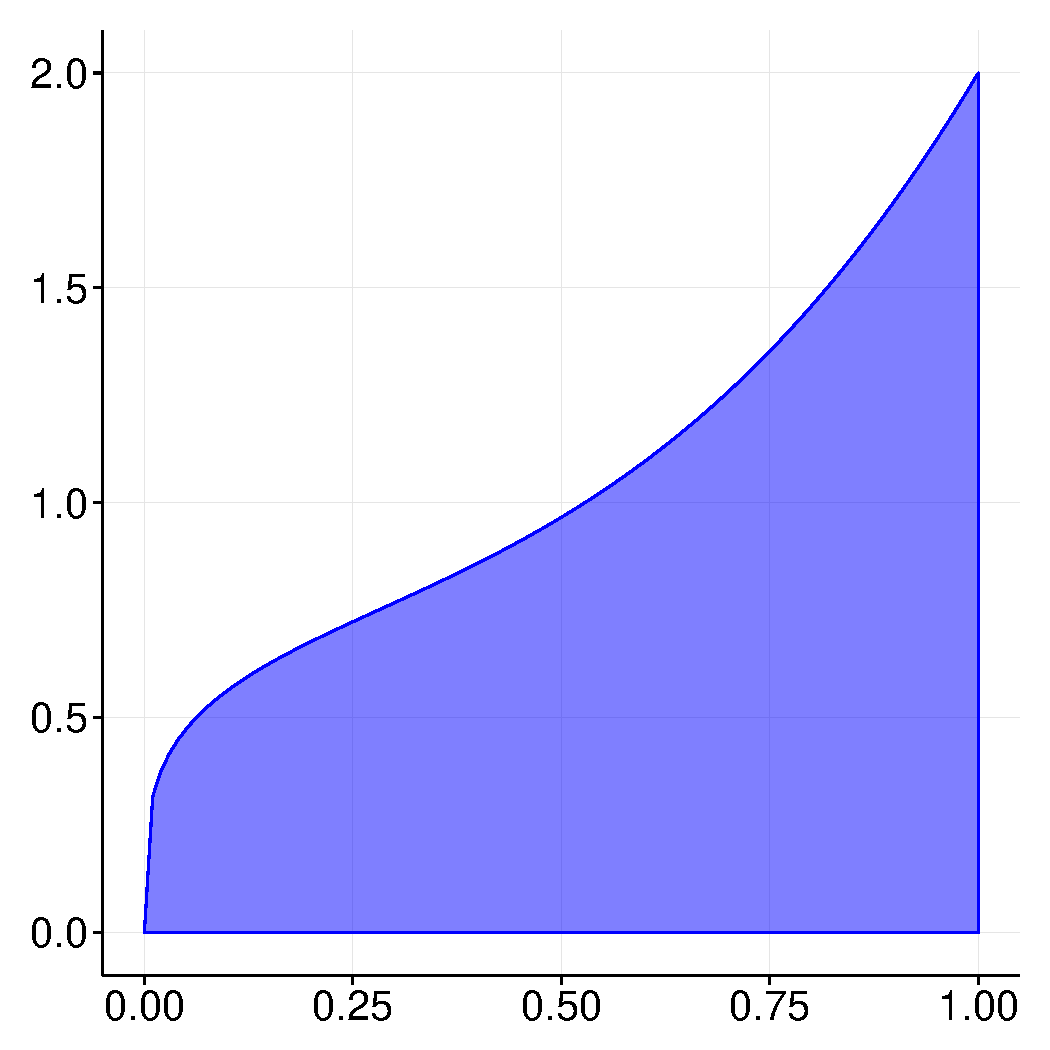
\includegraphics[width=0.45\textwidth,page=1]{ex_int.pdf}
\includegraphics[width=0.45\textwidth,page=2]{ex_int.pdf}
\end{center}
Your family just moved to a new apartment in Zurich and now it is time to paint the walls to make your house more of a home. Your creative uncle gave you two interesting designs and since you have two $1x2 m$ walls in your house, why not paint one wall with one design and the other with the other? One detail: how can you make sure that your sister has a larger surface to paint than you? Just to help you a little bit: the equation of the left design is:
\begin{equation*}
f_{left}(x) = x^3 + \sqrt[4]{x}.
\end{equation*}
For the design on the right, the equation is:
\begin{equation*}
f_{right}(x) = x^6 + \sqrt[8]{x}.
\end{equation*}
\end{Exercise}

\begin{Answer}[ref=ex0202]
\noindent What we want to compare here is the surface of the design on the left:
\begin{equation*}
A_{left} = \int_{x=0}^1 f_{left}dx
\end{equation*}
with the surface of the one on the right:
\begin{equation*}
A_{right} = \int_{x=0}^1 f_{right}dx
\end{equation*}
First we look for the primitive of $f_{left}(x)$. Realise that we can write this function as follows:
\begin{equation*}
f_{left}(x) = x^3 + \sqrt[4]{x} = x^3 + x^{\frac{1}{4}}.
\end{equation*}
For this function we find:
\begin{equation*}
F_{left}(x) = \frac{1}{4} x^4 + \frac{4}{5}x^{\frac{5}{4}}.
\end{equation*}
The total surface to paint in this design is thus:
\begin{equation*}
A_{left} = F_{left}(1) - F_{left}(0) = \frac{1}{4} + \frac{4}{5} - 0 = \frac{21}{20} = 1.05.
\end{equation*}
We repeat the same procedure for the right design. First we rewrite the expression:
\begin{equation*}
f_{right}(x) = x^6 + \sqrt[8]{x} = x^6 + x^{\frac{1}{8}}.
\end{equation*}
Next, we find the primitive of this function:
\begin{equation*}
F_{right}(x) = \frac{1}{7}x^7 + \frac{8}{9}x^{\frac{9}{8}}.
\end{equation*}
Now it is easy to find the total surface for this design:
\begin{equation*}
A_{right} = F_{right}(1) - F_{right}(0)  = \frac{1}{7} + \frac{8}{9} - 0 = \frac{65}{63} \approx 1.03.
\end{equation*}
So it turns out that the design on the right is slightly smaller. Although I wonder whether this really makes the difference... At least you practiced integration.
\end{Answer}

\begin{Exercise}[title=Find the primitives of the following functions, difficulty=2,label=ex3]
\begin{align*}
a(x) & =2 & e(x) &= x^6-2x^3+\frac{2}{3}\\ 
b(x) & =x^3 & f(x) &= \sqrt[]x\\  
c(x) &=3x^2-6 & g(x) &=\sqrt[]x+ \sqrt[3]x\\
d(x) &= -\frac{3}{4}x^2+x-6 &  h(x) &=\frac{5}{6}\sqrt[5]{x}+2\\  
\end{align*}
\end{Exercise}

\begin{Answer}[ref=ex3]
\noindent a(x) is the simplest primitive:
\begin{align*}
a(x) &= 2 & &\rightarrow& & A(x) = 2x + c
\end{align*}
For the next four questions, you need to use the power rule of integration.
\begin{align*}
b(x) &= x^3 & & \rightarrow & B(x)&=\frac{1}{4}x^4+c\\[1ex]
c(x) &= 3x^2-6 & &\rightarrow &C(x)&=x^3-6x+c\\[1ex]
d(x) &= \-\frac{3}{4}x^2+x-6 & & \rightarrow & D(x)&= -\frac{3}{4}\cdot \frac{1}{3}x^3+\frac{1}{2}x^2-6x+c\\
& & & & &=-\frac{1}{4}x^3+\frac{1}{2}x^2-6x+c\\[1ex]
e(x) &= x^6-2x^3+\frac{2}{3} & & \rightarrow & E(x)&=\frac{1}{7}x^7-\frac{1}{4}2x^4+\frac{2}{3}x+c\\
& & & & &=\frac{1}{7}x^7-\frac{1}{2}x^4+\frac{2}{3}x+c
\end{align*}
For the last three questions, you need no more than the power rule but you have to rearrange your equations first to rewrite the square root as a simple power. 
\begin{align*} 
f(x) &= \sqrt[]x & f(x)&= x^\frac{1}{2}& & \rightarrow & 
F(x)&=\frac{2}{3}x^\frac{3}{2}+c \\
& & & & & & &=\frac{2}{3}\sqrt[]{x^3}+c\\[1ex]
g(x) &= \sqrt[]x+ \sqrt[3]x & g(x)&= x^\frac{1}{2}+ x^\frac{1}{3}& & \rightarrow & G(x) &=\frac{2}{3}x^\frac{3}{2}+\frac{3}{4}x^\frac{4}{3}+c\\
& & & & & & &=\frac{2}{3}\sqrt[]{x^3}+\frac{3}{4}\sqrt[3]{x^4}+c\\[1ex]
 h(x) &=\frac{5}{6}\sqrt[5]{x}+2 & h(x) &=\frac{5}{6}x^\frac{1}{5}+2 & & \rightarrow & H(x)&=\frac{5}{6}\cdot \frac{5}{6}x^\frac{6}{5}+2x+c\\
& & & & & & &=\frac{25}{36}x^\frac{6}{5}+2x+c
\end{align*}
Well, we have to admit that for that last one it was tempting to think that the fraction would disappear. Unfortunately the rules for integration are in this case more important than gut feelings...
\end{Answer}

\begin{Exercise}[title=A different shape, difficulty=3,label=ex1202]
\begin{center}
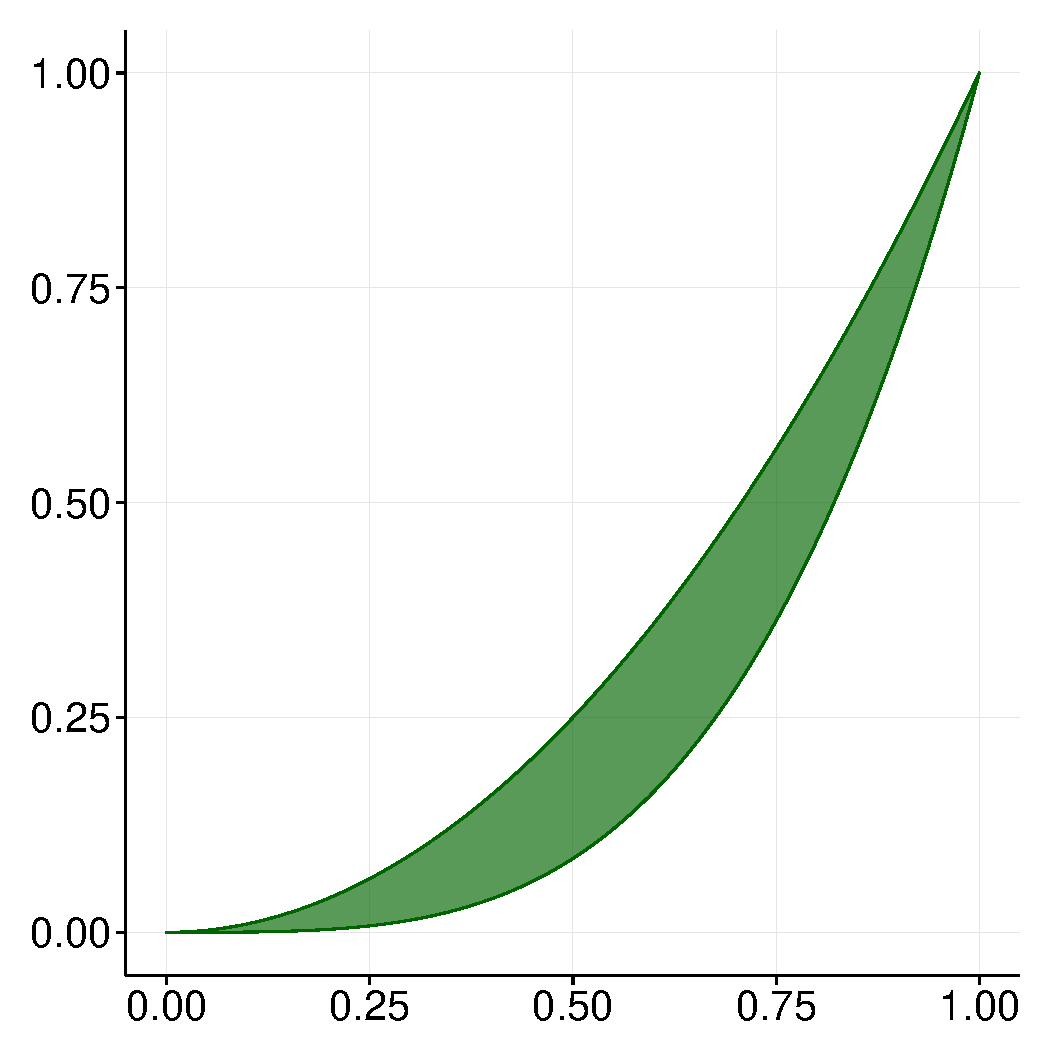
\includegraphics[width=0.45\textwidth,page=1]{ex_int2.pdf}
\end{center}
Can you calculate the surface of the shape above? To help you, we will reveal that the curve that describes the upper boundary of the shape is given by:
\begin{equation*}
f_{top}(x) = x^2
\end{equation*}
and the curve describing the lower boundary of the shape is given by:
\begin{equation*}
f_{bottom}(x) = x^4-\frac{1}{4}x^5+\frac{1}{4}x^3.
\end{equation*}

\end{Exercise}

\begin{Answer}[ref=ex1202]
\noindent First we calculate the surface between the upper boundary and the $x$-axis, from this we substract the surface below the lower boundary of the shape:
\begin{equation*}
A = \int_{x=0}^1 f_{top}(x) dx - \int_{x=0}^1 f_{bottom}(x) dx = (F_{top}(1)-F_{top}(0))-(F_{bottom}(1)-F_{bottom}(0)). 
\end{equation*}
The primitive for the upper boundary:
\begin{equation*}
F_{top}(x) = \frac{1}{3}x^3.
\end{equation*}
And thus:
\begin{equation*}
A_{top} = F_{top}(1) - F_{top}(0) = \frac{1}{3}.
\end{equation*}
For the primitive of the lower boundary:
\begin{equation*}
F_{bottom} = \frac{1}{5}x^5 - \frac{1}{24}x^6 + \frac{1}{16}x^4.
\end{equation*}
And thus:
\begin{equation*}
A_{bottom} = F_{bottom}(1) - F_{bottom}(0) = \frac{1}{5} - \frac{1}{24} + \frac{1}{16} = \frac{15}{240} - \frac{10}{240} + \frac{48}{240} = \frac{53}{240} \approx 0.22.
\end{equation*}
The surface of the shape is thus:
\begin{equation*}
A = A_{top} - A_{bottom} = \frac{1}{3} - \frac{53}{240} = \frac{80}{240} - \frac{53}{240} = \frac{27}{240} = \frac{9}{80} = 0.1125.
\end{equation*}

\end{Answer}

%%%%%%% DIFF EQN %%%%%%%%%%%%%%%%%%%%%%%%%%%%%%%%%%%

\section{Differential Equations}

\subsection{The Exponential Function}

An exponential functions look similar to a power function except that the variable of interest, $x$, is the exponent rather than the base. Exponential functions are functions of the form $f(x)=a^x$, here $a$ is a positive constant. Graphically, an exponential function looks like the graph below. At low values of x, the curve is very close to one (because $a^0=1$). When $x$ increases by $1$, the value of $f(x)$ is multiplied by $a$, or mathematically put:
\begin{equation}
f(x+1) = a \cdot f(x).
\end{equation}
Therefore exponential functions are used to model system where a the factor of increase is constant.\\ 
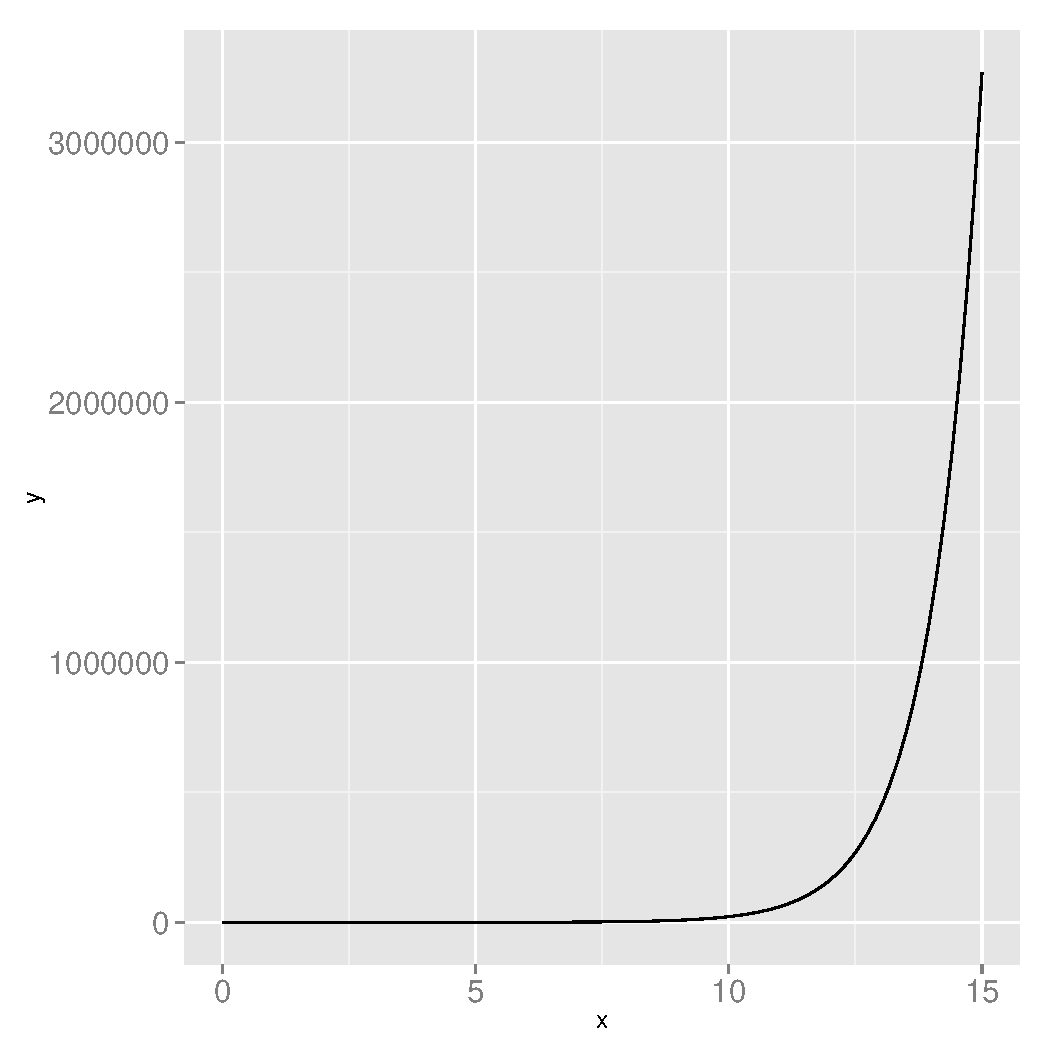
\includegraphics[width=0.85\textwidth]{exponential_plot.pdf}\\


\textbf{The function} $f(x) = A \cdot e^x$


Most of the time, the exponential function refers to the natural exponential function, an exponential function in base $e$ ($e \approx 2.72$) multiplied by a constant ($A$); $A \cdot e^x$. When $x$ tends towards $\infty$, $A \cdot e^x$ also tends towards $\infty$. This function is of specic interest to describe population growth and you will see it many times in the rest of this course. An important property of the exponential function is that its derivative is the same as the original function:
\begin{align}
f(x)& = A \cdot e^x & &\rightarrow& & f^\prime(x) =  A \cdot e^x  
\end{align}

It means that \textbf{the slope of the graph at any point is the $y$ value at that
point}. It follows from this that the integral is also identical to the original function.
\begin{align}
f(x)& = A \cdot e^x & &\rightarrow& &F(x) =  A \cdot e^x  + c
\end{align}
Of course for this exponential funciton, the chain rule is still balid:
\begin{align}
f(x)& = A \cdot e^u(x) & &\rightarrow& & f^\prime(x) = u^\prime(x)f^\prime(u) = u^\prime(x)A \cdot e^{ux} 
\end{align}
If $u(x)=kx$, with $k$ a constant, this means that:
\begin{align}
f(x)& = A \cdot e^kx & &\rightarrow& & f^\prime(x) = u^\prime(x)f^\prime(u) = u^\prime(x)A \cdot e^{ux} 
\end{align}
This is of interest because if the increase of a variable (e.g. population size over time $N(t)$) is proportional to the size of the variable, this means that:
\begin{equation}
N^\prime(t)=k \cdot N(t).
\end{equation}
This equation is called a dierential equation because it contains both a function and the derivative of that function. For this dierential equation we know that it describes exactly the property of the exponential function, we thus know that $N(t)$ is an exponential function:
\begin{equation}
N(t)=A \cdot e^{k \cdot t}.
\end{equation}

\subsection{The Logarithmic Function}
Just like division is the inverse operation of multiplication, the logarithm is the inverse operation of an exponential. If $a^x=b$, then $\log_b(a)=x$. The logarithm $\log_a(b)$ gives the power at which we need to elevate the base ($a$) to get $b$. Based on this definition one can find that:
\begin{equation*}
a^{\log_a(b)} = \log_a(a^b) = b.
\end{equation*}

\textbf{The natural logarithm}\\
The logarithm of special interest for us is the natural logarithm $ln(y)$ which is the inverse operation of the natural exponential function $e^x$. If $ln(y) = x$, then $e^x = y$. The notation $ln$ is specic to the natural logarithm and is always in base $e$. However, the literature can be confusing as you may see $log(y)$ to mean $ln(y)$ or $log(y)$ to mean $log_{10}(y)$. However, most of the time you can figure it out from the context.\\
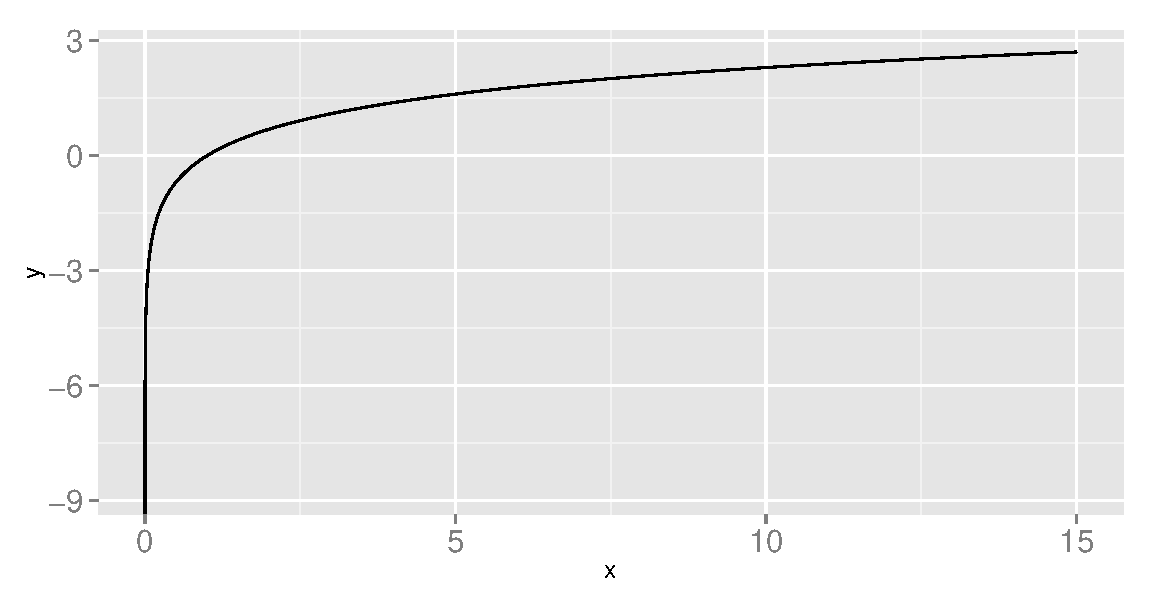
\includegraphics[width=0.85\textwidth]{ln_plot.pdf}\\
The figure above shows the curve of a natural logarithmic function. The closer $x$ is to zero, the faster the value of $ln(x)$ gets smaller. Conversly, when $x$ is far from zero, the value of $ln(x)$ keeps increasing but the larger $x$, the slower this increase. The limit of $ln(x)$ as $x$ approaches infinity is equal to infinity.\\

\begin{mdframed}
\textbf{Use of the natural logarithm}\\
Let us take the function $f(x)= e^{0.33\cdot x}$, which is a typical growth function in ecology. This function is plotted in the graph below.\\
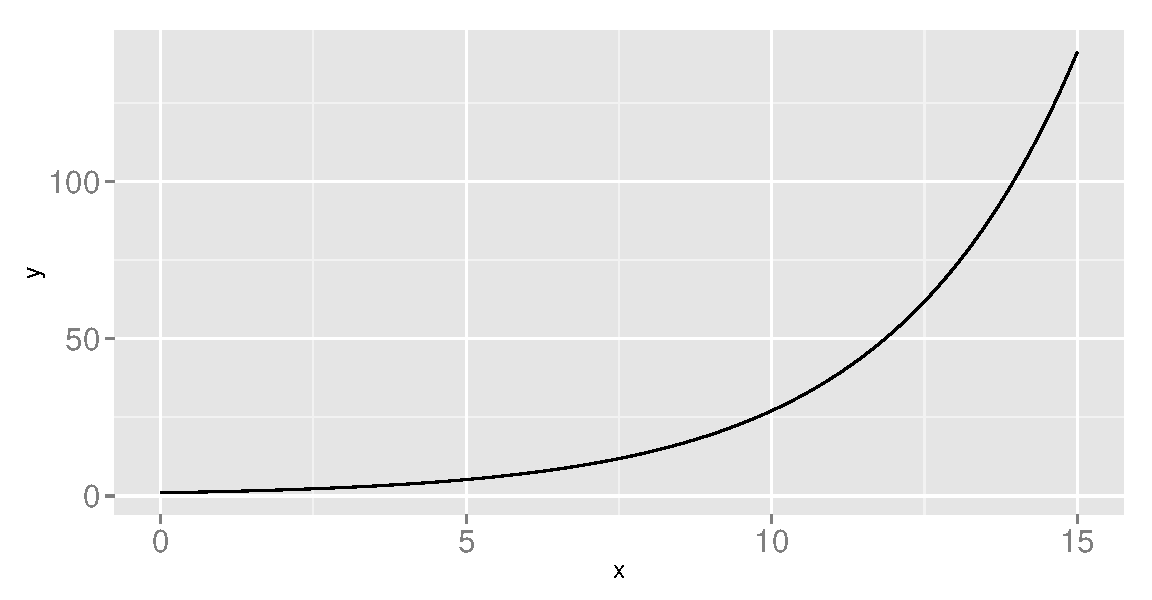
\includegraphics[width=0.85\textwidth]{example_e_plot.pdf}\\
This exponetially growing curve is nice but not very convinient to work with. A straight line would be much easier. The same graph can be made into a straight line with the use of the natural logarithmic function which is the inverse of the exaponential. This is what you see in the graph below\\
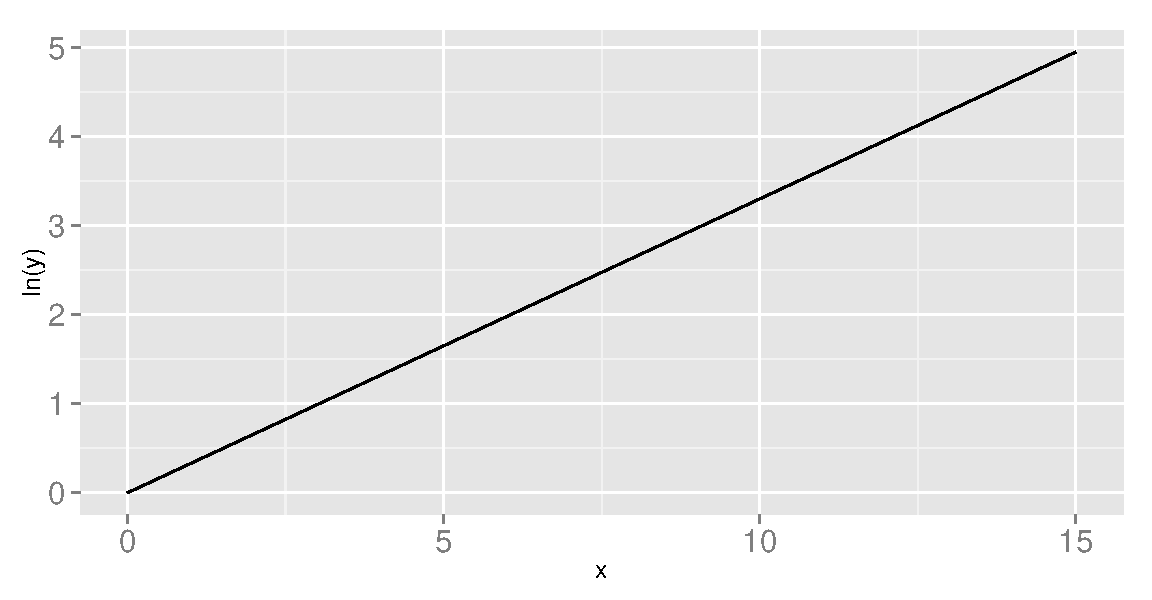
\includegraphics[width=0.85\textwidth]{example_ln_plot.pdf}\\
So what is the function of this graph? It is $ln(f(x))$, which is
\begin{equation}
\begin{aligned}
\ln(f(x))&=\ln(e^{0.33\cdot x})\\
&=0.33\cdot x 
\end{aligned}
\end{equation}
Visually and computationally,  it is much easier to find the function of a straight line and then find the initial function. This is why the natural loragithm is frequently used in combination with the exponential. 
\end{mdframed}


\subsection{Exercises}
\begin{Exercise}[title= Answer the following questions,label=exexln,difficulty=1]
\Question Around the exponential\\ 
\subQuestion Solve for $x$ the following equations
\begin{align*}
2^x &= 4			&  2\cdot 3^x&=18 \\
e^x &= 1			&  x^e&=4
\end{align*}
\subQuestion Find the derivatives of the following functions
\begin{align*}
a(x) &= 5\cdot e^x			&  b(x)&=e^x + x^2 
\end{align*}
\subQuestion Draw the function $e^x$. Describe what happwns when $x$ is very small ($x=- \infty$) and when $x$ is very large ($x=+\infty$).
\Question Around the logarithm
\subQuestion Solve for $x$ the following equations
\begin{align*}
\log_2{x} &= 4			& \log_5{x} &=3 \\
\ln(x) &= 1			&  \ln(x)&=3
\end{align*}
\subQuestion Draw the function $\ln(x)$. Describe what happens when $x<0$ and $x$ is very large ($x=+\infty$).

\Question Exponential and logarithm combined
\subQuestion Draw the function $\ln(e^{0.4x})$.
\subQuestion What is special about that function?
\end{Exercise}
\begin{Answer}[ref=exexln]
\Question Around the exponential\\ 
\subQuestion Solve for $x$ the following equations
\begin{eqnarray*}
2^x&=&4\\
x&=&\log_2(4)\\
x=2
\end{eqnarray*}
\begin{eqnarray*}
2 \cdot 3^x &=&18\\
3^x&=&9\\
x&=& \log_3(9)\\
x&=&2
\end{eqnarray*}
\begin{eqnarray*}
e^x &=&1\\
\ln(1)&=&x\\
x&=&0
\end{eqnarray*}
\begin{eqnarray*}
e^x &=&4\\
\ln(4)&=&x\\
x&=&1.386
\end{eqnarray*}
\subQuestion Find the derivatives of the following functions
\begin{align*}
a^\prime(x) &= 5\cdot e^x			&  b^\prime(x)&=e^x + 2x 
\end{align*}
\subQuestion Draw the function $e^x$. Describe what happwns when $x$ is very small ($x=- \infty$) and when $x$ is very large ($x=+\infty$).\\
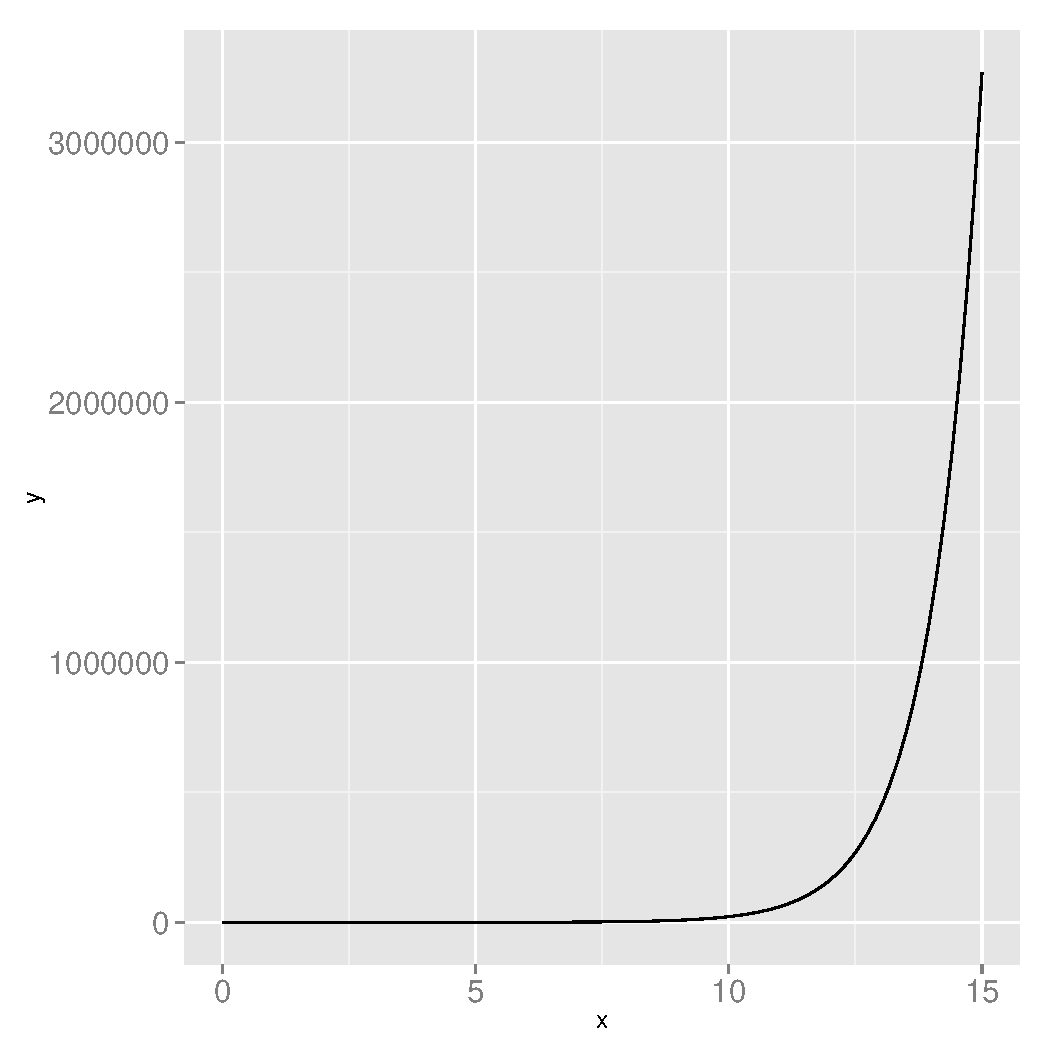
\includegraphics[width=0.85\textwidth]{exponential_plot.pdf}\\
When $x$ is very small, the function tend towards $1$ and when $x$ is very large the function tends towards infinity.
\Question Around the logarithm
\subQuestion Solve for $x$ the following equations
\begin{eqnarray*}
\log_2{x} &= &4\\
x&=&2^4\\
x&=&16
\end{eqnarray*}
\begin{eqnarray*}
\log_5{x} &= &3\\
x&=&5^3\\
x&=&125
\end{eqnarray*}
\begin{eqnarray*}
\ln(x) &= &1\\
x&=&e^1\\
x&=&e
\end{eqnarray*}
\begin{eqnarray*}
\ln(x) &= &3\\
x&=&e^3\\
x&=&20.086
\end{eqnarray*}
\subQuestion Draw the function $\ln(x)$. Describe what happens when $x<0$ and $x$ is very large ($x=+\infty$).\\
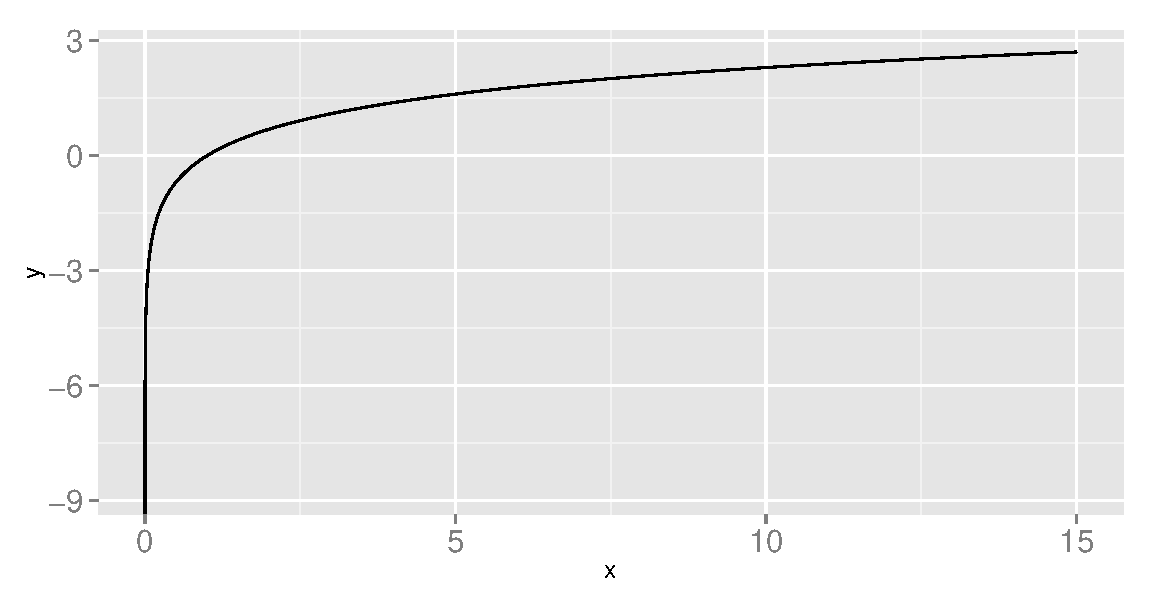
\includegraphics[width=0.85\textwidth]{ln_plot.pdf}\\
The logarithmic function is undefined at $x<0$ and tends towards infinty fir large value of $x$.

\Question Exponential and logarithm combined
\subQuestion Draw the function $\ln(e^{0.4x})$.\\
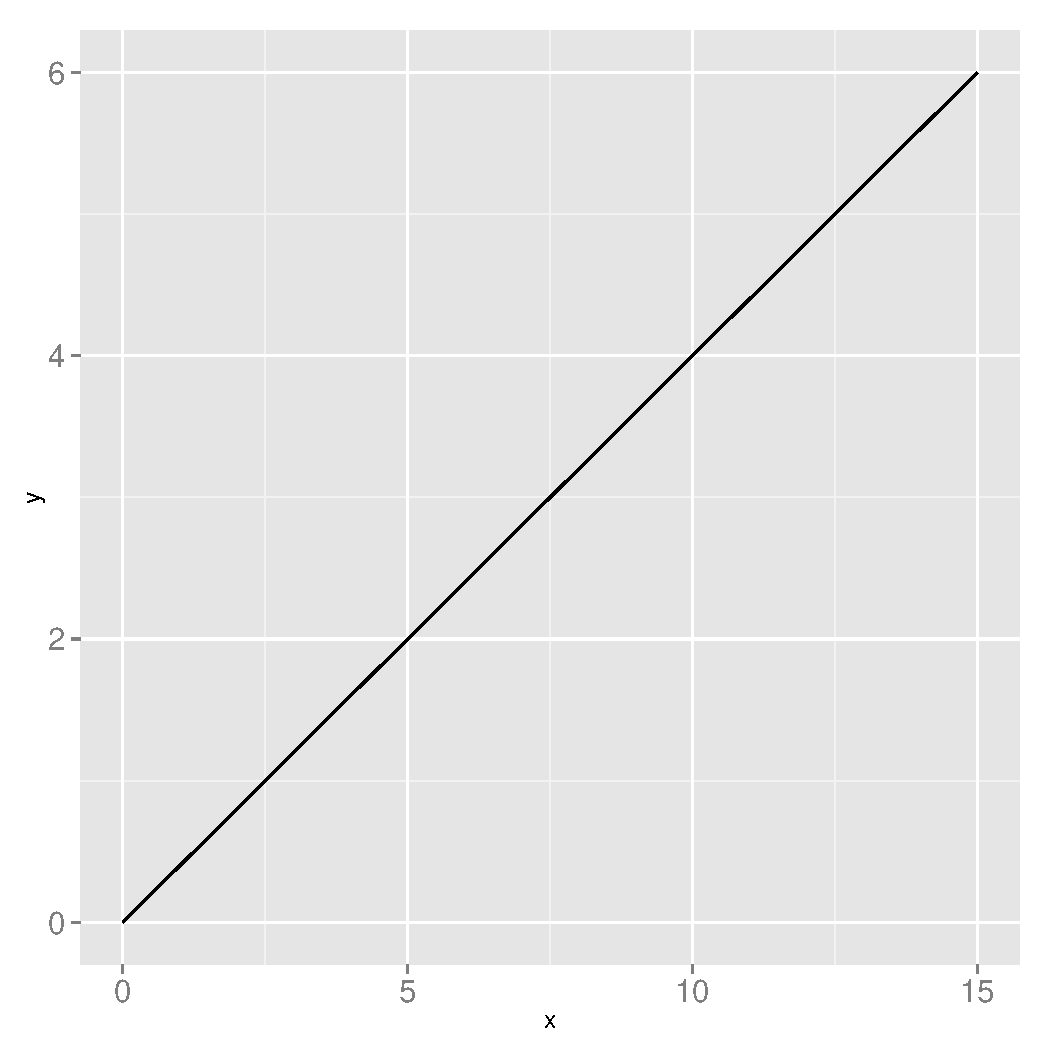
\includegraphics[width=0.85\textwidth]{ex_exp_ln_plot.pdf}\\
\subQuestion What is special about that function?\\
It is a straight line.
\end{Answer}

%%%%%%%%%%%%%%%%%%%%%%%%%%%%%%%%%%%%%%%%%%%%%%%%%%%
%%%%%%% MATRIX ALG %%%%%%%%%%%%%%%%%%%%%%%%%%%%%%%%%%%
%%%%%%%%%%%%%%%%%%%%%%%%%%%%%%%%%%%%%%%%%%%%%%%%%%%

\chapter{Introduction to Matrix Algebra}
\section{Vectors}

\subsection{Graphically}
Vectors are probably the easiest to understand graphically. We drew an example of a vector below. Informally you could say that a vector is an arrow, for this reason usually when something is a vector, a small arrow is put on top of it to indicate that it is a vector: $\vec{v}$. It is different from a 'normal' number (a scalar) in the respect that a vector can not be described with one single number. We could give you the length of a vector, but you would still not know in which direction it points. On the other hand, we could specify what a vector points at, but you would still not know how long it is. \textbf{A vector is described by two components: a length and a direction.} The most common example of a vector is velocity: when you move around in a car there are two important components: your speed (the length of the vector) and your direction. \newline
\begin{center}
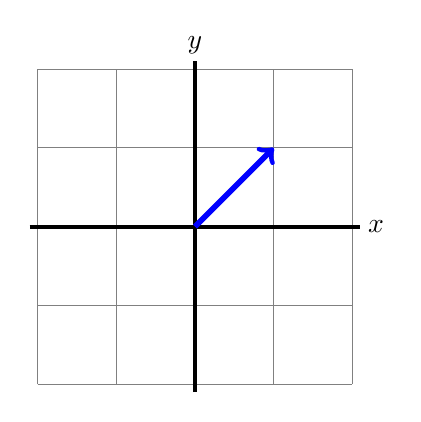
\begin{tikzpicture}

\draw[step=1.0,gray,thin] (-2,-2) grid (2,2);
\draw[black, line width=0.05 cm] (-2.1,0) -- (2.1,0);
\draw[black, line width=0.05 cm] (0,-2.1) -- (0,2.1);
\node at (0,2.3) {$y$};
\node at (2.3,0) {$x$};

\draw[blue, line width=0.07 cm,->] (0,0) -- (1,1);
\end{tikzpicture}
\end{center}
%%%%%%%%%%%%%%%%%%%%%%%%%%%%%%%%%%%% WITH NUMBERS%%%%%%%%%%%%%%%%%%%%%%%
\subsection{With numbers} 
Pictures are easy to understand, but not always easy to use in communication. When a researcher here in Z\"urich wants to share one of his results with a collaborator on the other side of the ocean, it is a bit impractical to send a collection of drawings. Instead it would be nice to just send a few numbers per e-mail. In this case the researcher would have to send both bits of information: the direction and the length of the vector ($\vec{v}$). Sending the length (we write this as $\left|\vec{v}\right|$) is straightforward, the direction can be specified as the angle ($\theta$) between the vector and the $x$-axis:

\begin{center}
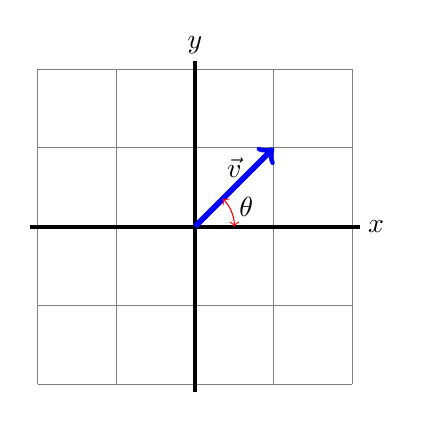
\begin{tikzpicture}
\draw[step=1.0,gray,thin] (-2,-2) grid (2,2);
\draw[black, line width=0.05 cm] (-2.1,0) -- (2.1,0);
\draw[black, line width=0.05 cm] (0,-2.1) -- (0,2.1);
\node at (0,2.3) {$y$};
\node at (2.3,0) {$x$};
\node at (0.5,0.75) {$\vec{v}$};
\draw[blue, line width=0.07 cm,->] (0,0) -- (1,1);
 \draw[red,<->]  (0.5,0) arc (0:45:0.5);
 \node at (0.65,0.25) {$\theta$};
\end{tikzpicture}
\end{center}

However, measuring angles can be annoying, so therefore a different notation is more frequently used. In this notation the part of the vector along the x-axis ($v_x$) and the part along the y-axis ($v_y$) are recorded:
\begin{center}
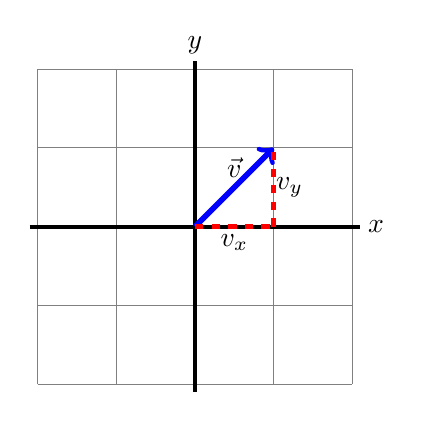
\begin{tikzpicture}
\draw[step=1.0,gray,thin] (-2,-2) grid (2,2);
\draw[black, line width=0.05 cm] (-2.1,0) -- (2.1,0);
\draw[black, line width=0.05 cm] (0,-2.1) -- (0,2.1);
\node at (0,2.3) {$y$};
\node at (2.3,0) {$x$};
\node at (0.5,0.75) {$\vec{v}$};
\draw[blue, line width=0.07 cm,->] (0,0) -- (1,1);
\draw[red,dashed,line width = 0.06 cm]  (0,0) -- (1,0);
\draw[red,dashed, line width=0.06 cm] (1,0) -- (1,1);
\node at (0.5,-0.2) {$v_x$};
\node at (1.2,0.5) {$v_y$};
\end{tikzpicture}
\end{center}
This is usually written down as follows:
\begin{equation}
\vec{v} = 
\begin{pmatrix}
v_x \\
v_y
\end{pmatrix}
\label{vector}
\end{equation}
\clearpage
\begin{mdframed}
The two notations can be converted into one another. Using the Pythagorean theorem ($a^2+b^2 = c^2$), one can see that for the length of the vector:
\begin{equation*}
|\vec{v}| = \sqrt{v_x^2 + v_y^2}
\end{equation*}
Those who still remember the basics of trigonometry, will (hopefully) agree that for the angle $\theta$ the following equation holds:
\begin{equation*}
tan(\theta) = \frac{v_y}{v_x}
\end{equation*}
$\;$
\end{mdframed}
%%%%%%%%%%%%%%%%%%%%%%%%%%%% GRAPHICAL ADDITION %%%%%%%%%%%%%%%%%%%%%%%
\subsection{Graphical addition}
So far we have focused on one single vector. We will now slowly increase the excitement by doubling the number of vectors that we work with. Below two vectors are drawn: $\vec{u}$ and $\vec{v}$:
\begin{center}
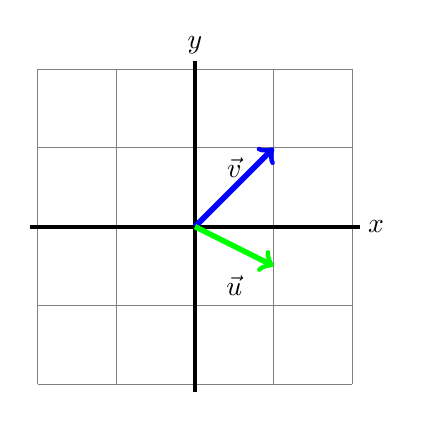
\begin{tikzpicture}

\draw[step=1.0,gray,thin] (-2,-2) grid (2,2);
\draw[black, line width=0.05 cm] (-2.1,0) -- (2.1,0);
\draw[black, line width=0.05 cm] (0,-2.1) -- (0,2.1);
\node at (0,2.3) {$y$};
\node at (2.3,0) {$x$};

\node at (0.5,0.75) {$\vec{v}$};
\draw[blue, line width=0.07 cm,->] (0,0) -- (1,1);

\node at (0.5,-0.75) {$\vec{u}$};
\draw[green, line width=0.07 cm, ->] (0,0) -- (1,-0.5);
\end{tikzpicture}
\end{center}
Like we can add up numbers ($4+2=6$), we can also add up vectors. To do so in a drawing, we move the second vector such that it begins where the first one ends. The sum of the two vectors is the vector that starts at the origin ($(0,0)$) and ends where the second vector is pointing. Words are sometimes fuzzy so let's instead look at a picture.
\begin{center}
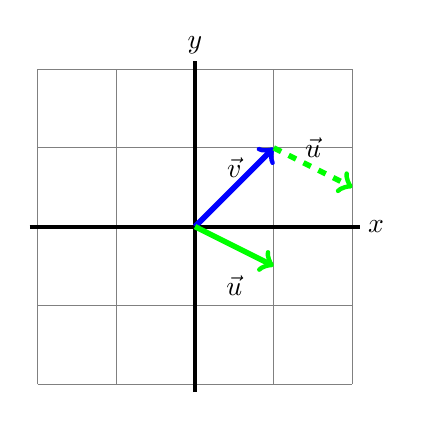
\begin{tikzpicture}

\draw[step=1.0,gray,thin] (-2,-2) grid (2,2);
\draw[black, line width=0.05 cm] (-2.1,0) -- (2.1,0);
\draw[black, line width=0.05 cm] (0,-2.1) -- (0,2.1);
\node at (0,2.3) {$y$};
\node at (2.3,0) {$x$};

\node at (0.5,0.75) {$\vec{v}$};
\draw[blue, line width=0.07 cm,->] (0,0) -- (1,1);

\node at (0.5,-0.75) {$\vec{u}$};
\draw[green, line width=0.07 cm, ->] (0,0) -- (1,-0.5);

\node at (1.5,1) {$\vec{u}$};
\draw[green, dashed, line width=0.07 cm, ->] (1,1) -- (2,0.5);

\end{tikzpicture}
\hspace{1cm}
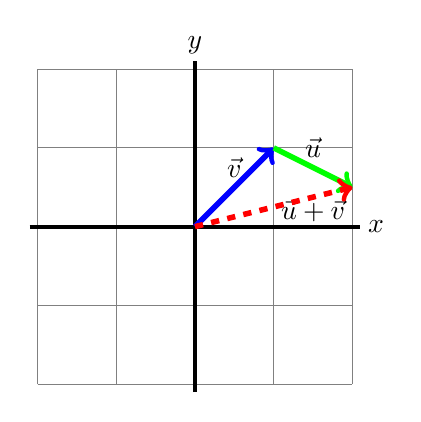
\begin{tikzpicture}

\draw[step=1.0,gray,thin] (-2,-2) grid (2,2);
\draw[black, line width=0.05 cm] (-2.1,0) -- (2.1,0);
\draw[black, line width=0.05 cm] (0,-2.1) -- (0,2.1);
\node at (0,2.3) {$y$};
\node at (2.3,0) {$x$};

\node at (0.5,0.75) {$\vec{v}$};
\draw[blue, line width=0.07 cm,->] (0,0) -- (1,1);

\node at (1.5,1) {$\vec{u}$};
\draw[green, line width=0.07 cm, ->] (1,1) -- (2,0.5);

\node at (1.5,0.2) {$\vec{u}+\vec{v}$};
\draw[red,dashed, line width=0.07 cm, ->] (0,0) -- (2,0.5);
\end{tikzpicture}
\end{center}
In the left picture, first the second vector is moved such that it begins at the end of the first vector. Next, the sum of the two vectors is drawn from the origin to where the second vector is now pointing.
\begin{mdframed}
Please note that it is not important which vector is the first and which vector is the second vector. If we would have called $\vec{v}$ the second vector and $\vec{u}$ the first, the result would have been exactly the same:
\begin{center}
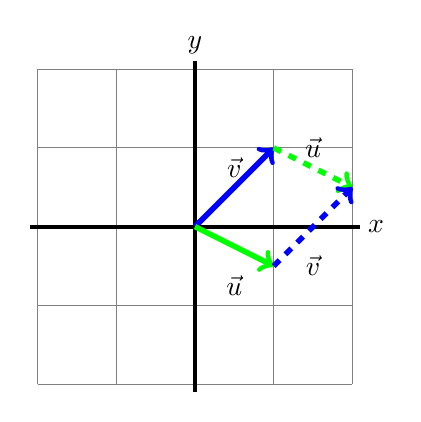
\begin{tikzpicture}

\draw[step=1.0,gray,thin] (-2,-2) grid (2,2);
\draw[black, line width=0.05 cm] (-2.1,0) -- (2.1,0);
\draw[black, line width=0.05 cm] (0,-2.1) -- (0,2.1);
\node at (0,2.3) {$y$};
\node at (2.3,0) {$x$};

\node at (0.5,0.75) {$\vec{v}$};
\draw[blue, line width=0.07 cm,->] (0,0) -- (1,1);

\node at (0.5,-0.75) {$\vec{u}$};
\draw[green, line width=0.07 cm, ->] (0,0) -- (1,-0.5);

\node at (1.5,1) {$\vec{u}$};
\draw[green, dashed, line width=0.07 cm, ->] (1,1) -- (2,0.5);

\node at (1.5,-0.5) {$\vec{v}$};
\draw[blue, dashed, line width=0.07 cm, ->] (1,-0.5) -- (2,0.5);
\end{tikzpicture}
\end{center}
Hopefully from this picture it has become clear that in general:
\begin{equation*}
\vec{v} + \vec{u} = \vec{u} + \vec{v}
\end{equation*}
\end{mdframed}
\subsection{Addition}
Fortunately addition of two vectors becomes very easy when we use the notation from equation \ref{vector}:
\begin{equation}
\vec{u} + \vec{v} = 
\begin{pmatrix}
u_x\\
u_y
\end{pmatrix}
+
\begin{pmatrix}
v_x\\
v_y
\end{pmatrix}
=
\begin{pmatrix}
u_x + v_x \\
u_y + v_y
\end{pmatrix}
\end{equation}
That is: we can simply add up the separate x contributions to get the total x contribution of the sum of the vectors and the y contributions to get the y contribution of the sum of the vectors.
\subsection{Multiplication of a vector by a scalar}
Sometimes you want to express that the length of a vector changes while the direction of that vector does not change. An example is speeding up in a car: your speed increases but as long as you do not use the steering wheel your direction will (hopefully) remain the same. In the following images we illustrate the multiplication of the vector $\vec{v}$ by a scalar $a$. If this scalar is negative, the multiplication will make the vector point in the opposite direction.
\begin{center}
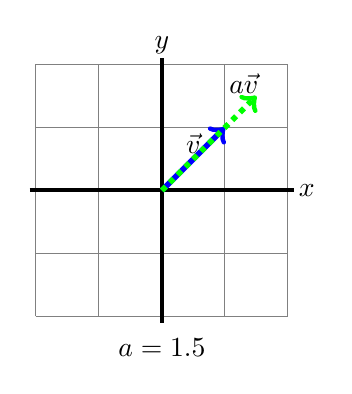
\begin{tikzpicture}[scale=0.8]
\draw[step=1.0,gray,thin] (-2,-2) grid (2,2);
\draw[black, line width=0.05 cm] (-2.1,0) -- (2.1,0);
\draw[black, line width=0.05 cm] (0,-2.1) -- (0,2.1);
\node at (0,2.3) {$y$};
\node at (2.3,0) {$x$};

\node at (0.5,0.75) {$\vec{v}$};
\draw[blue, line width=0.07 cm,->] (0,0) -- (1,1);
\draw[green, line width=0.07 cm, ->,dotted] (0,0) -- (1.5,1.5);
\node at (0,-2.5) {$a=1.5$};
\node at (1.3,1.7) {$a\vec{v}$};
\end{tikzpicture}
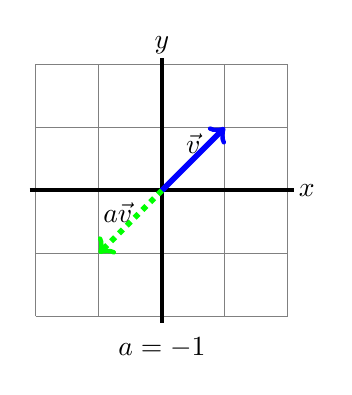
\begin{tikzpicture}[scale=0.8]
\draw[step=1.0,gray,thin] (-2,-2) grid (2,2);
\draw[black, line width=0.05 cm] (-2.1,0) -- (2.1,0);
\draw[black, line width=0.05 cm] (0,-2.1) -- (0,2.1);
\node at (0,2.3) {$y$};
\node at (2.3,0) {$x$};

\node at (0.5,0.75) {$\vec{v}$};
\draw[blue, line width=0.07 cm,->] (0,0) -- (1,1);
\draw[green, line width=0.07 cm, ->,dotted] (0,0) -- (-1,-1);
\node at (0,-2.5) {$a=-1$};
\node at (-0.7,-0.35) {$a\vec{v}$};
\end{tikzpicture}
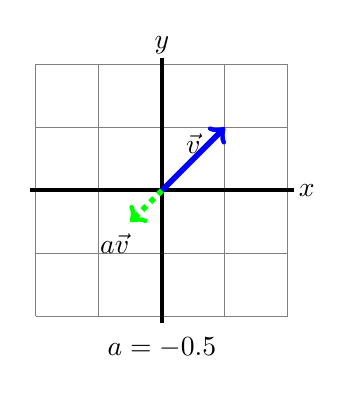
\begin{tikzpicture}[scale=0.8]
\draw[step=1.0,gray,thin] (-2,-2) grid (2,2);
\draw[black, line width=0.05 cm] (-2.1,0) -- (2.1,0);
\draw[black, line width=0.05 cm] (0,-2.1) -- (0,2.1);
\node at (0,2.3) {$y$};
\node at (2.3,0) {$x$};

\node at (0.5,0.75) {$\vec{v}$};
\draw[blue, line width=0.07 cm,->] (0,0) -- (1,1);
\draw[green, line width=0.07 cm, ->,dotted] (0,0) -- (-0.5,-0.5);
\node at (0,-2.5) {$a=-0.5$};
\node at (-0.75,-0.85) {$a\vec{v}$};
\end{tikzpicture}
\end{center}
When facing numbers instead of figures, the multiplication of a vector with a scalar is performed by simply multiplying the separate elements of the vector by that scalar. That is:
\begin{equation}
a\vec{v} = a
\begin{pmatrix}
v_x \\
v_y
\end{pmatrix}
=
\begin{pmatrix}
a \cdot v_x \\
a \cdot v_y
\end{pmatrix}
\label{mult}
\end{equation}
\begin{mdframed}
We will now show that equation \ref{mult} indeed leads to a multiplication of the length of a vector, while its direction remains the same.

First, we know that for a vector $\vec{v}$ its length and direction are given as follows:
\begin{align*}
|\vec{v}| &= \sqrt{v_x^2 + v_y^2}\\
tan(\theta_v) &= \frac{v_y}{v_x}
\end{align*}
Let us now look at a new vector $\vec{u}$, where $\vec{u}=a\vec{v}$. That is: $\vec{u}$ is the vector $\vec{v}$ multiplied by a scalar. Now we know that:
\begin{equation*}
\vec{u} =
\begin{pmatrix}
u_x \\
u_y
\end{pmatrix}
= 
a \vec{v}
=
\begin{pmatrix}
a\cdot v_x\\
a\cdot v_y
\end{pmatrix}
\end{equation*}
And thus:
\begin{equation*}
|\vec{u}| = \sqrt{u_x^2 + u_y^2} = \sqrt{(a v_x)^2 + (a v_y)^2} = \sqrt{a^2 (v_x^2 + v_y^2)} = a \sqrt{v_x^2 + v_y^2} = a |\vec{v}| \\
\end{equation*}
\begin{equation*}
tan(\theta_u) = \frac{u_y}{u_x} = \frac{av_y}{av_x} = \frac{v_y}{v_x} = tan(\theta_v) 
\end{equation*}
We see that indeed both $\vec{v}$ and $\vec{u}$ have the same direction ($\theta$) but the length of $\vec{u}$ is a times the length of $\vec{v}$.
\end{mdframed}
\begin{mdframed}
To substract one vector from another is the same as adding up one vector to the negative version of the other, that is:
\begin{equation*}
\vec{u}-\vec{v} = \vec{u} + \left( -1 \cdot \vec{v}\right)
\end{equation*}
\end{mdframed}
\subsection{Larger dimensions}
So far we have been cocnerned only with two dimensional situation, not because these are the most relevant, but because these are the easiest to explain on paper. Fortunately it is relatively easy to extend everything we have discussed to 3 or even more dimensions. For every extra dimension that we add, we need to include one more number specifying the vector. That is, in three dimensions:
\begin{equation}
\vec{v} = \begin{pmatrix}
v_x \\
v_y \\
v_z
\end{pmatrix}
\end{equation}
Adding up vectors and multiplying them with scalars is just the same as in two dimensions:
\begin{equation}
\vec{v} + \vec{u} = \begin{pmatrix}
v_x \\
v_y \\
v_z
\end{pmatrix}
+
\begin{pmatrix}
u_x \\
u_y \\
u_z
\end{pmatrix}
=
\begin{pmatrix}
v_x + u_x \\
v_y + u_y\\
v_z + u_z
\end{pmatrix}
\end{equation}
\begin{equation}
a\vec{v} = a\begin{pmatrix} v_x \\ v_y \\ v_z \end{pmatrix} = \begin{pmatrix} a v_x \\ a v_y \\ a v_z \end{pmatrix}
\end{equation}
We could go to even more dimensions. Instead of the labels $x,y,z\dots$ we now number the different dimensions. If we have a total of $N$ dimensions, the following relations hold:
\begin{align}
\vec{v} &= \begin{pmatrix}v_1 \\ v_2 \\ \vdots \\ v_N\end{pmatrix}\\[1.5em]
\vec{v} + \vec{u} &= \begin{pmatrix}v_1 \\ v_2 \\ \vdots \\ v_N\end{pmatrix} + \begin{pmatrix}u_1 \\ u_2 \\ \vdots \\ u_N\end{pmatrix} = \begin{pmatrix}v_1 + u_1 \\ v_2 + u_2 \\ \vdots \\ v_N + u_N\end{pmatrix} \\[1.5em]
a\vec{v} & = a \begin{pmatrix}v_1 \\ v_2 \\ \vdots \\ v_N\end{pmatrix} = \begin{pmatrix}a v_1 \\ a v_2 \\ \vdots \\ a v_N\end{pmatrix}
\end{align}
\subsection{Basis Vectors}
A special group of vectors are the basis vectors, these are vectors with length 1 that point along one of the axis. We denote the $i^{th}$ basis vector as $\vec{e}_i$. In this notation we can use either numbers (1,2,3,..,N) or letters (x,y,z) for i. As an example we will show 3 basis vectors:
\begin{align*}
\vec{e}_x =& \vec{e}_1 = \begin{pmatrix} 1\\0\\ \vdots \\0 \end{pmatrix}, &
\vec{e}_y =& \vec{e}_2 = \begin{pmatrix} 0\\1\\0\\ \vdots \\0 \end{pmatrix}, &
& \vec{e}_N = \begin{pmatrix} 0\\ \vdots \\0 \\1 \end{pmatrix}
\end{align*}
This is just a definition that we will need in the next section. Note that there are as many basis vectors as there are dimensions: in 2 dimensional space there will only be two basis vectors ($\vec{e}_x$ and $\vec{e}_y$).
\subsection{Exercises}
%%%%%%%%%%%%%%%%%%%%%%%%%%%EXERCICE VECTORS%%%%%%%%%%%%%%
\begin{Exercise}[title= Answer the following questions,label=exVEC,difficulty=1]
\Question Vector manipulation\\ 
\subQuestion Draw the vectors $\vec{a} = \begin{pmatrix}
2 \\
3 
\end{pmatrix}$ and $\vec{b} = \begin{pmatrix}
-2 \\
-3 
\end{pmatrix}$
\subQuestion What is the angle between $\vec{a}$ and $\vec{b}$?
\subQuestion Draw the vector $\vec{a}+\vec{b}$ and then give the coordinates of that new vector. What is special about it?
\Question Vector addition\\
\subQuestion Draw the vectors $\vec{c} = \begin{pmatrix}
1 \\
1 
\end{pmatrix}$ and $\vec{d} = \begin{pmatrix}
-2 \\
3 
\end{pmatrix}$
\subQuestion Draw the vector $\vec{i}=\vec{c}-\vec{d}$ and then the vector $\vec{f}=\vec{d}-\vec{c}$. Give the coordinates for both vectors. Any comments?
\subQuestion Find the magnitude of $\vec{i}$, ($|\vec{i}|$).
\Question Vector multiplication
\subQuestion Draw $\vec{g} = \begin{pmatrix}
2 \\
4 
\end{pmatrix}$ 
\subQuestion Draw $2\vec{g}$ and give the coordinates of that new vector.
\Question Multiple dimensional vectors\\
\subQuestion What is the dimension of the following vector $h = \begin{pmatrix}
2 \\
3 \\
-4\\
-6
\end{pmatrix}$ ?
\subQuestion What are the coordinates of $5\vec{h}$?
\Question Basis vectors
\subQuestion In a two dimensional space, give the coordinates of the basis vectors in the first dimension ($\vec{e}_x$) and in the second dimension ($\vec{e}_y$)
\subQuestion What is special about these vectors?
\end{Exercise}

%%%%%%%%%%%%%%%%%%%%%ANSWER EXERCICE VECTORS%%%%%%%%%%%%%%
\begin{Answer}[ref=exVEC]
\Question Vector manipulation\\ 
\subQuestion Draw the vectors $\vec{a} = \begin{pmatrix}
2 \\
3 
\end{pmatrix}$ and $\vec{b} = \begin{pmatrix}
-2 \\
-3 
\end{pmatrix}$
\begin{center}

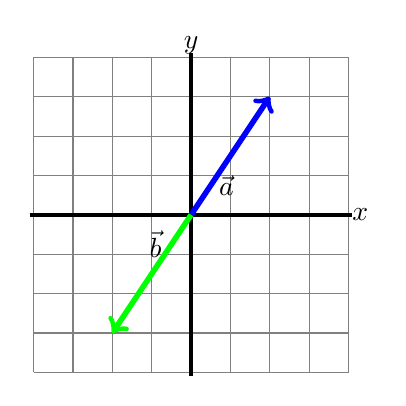
\begin{tikzpicture}[scale=0.5]

\draw[step=1.0,gray,thin] (-4,-4) grid (4,4);
\draw[black, line width=0.05 cm] (-4.1,0) -- (4.1,0);
\draw[black, line width=0.05 cm] (0,-4.1) -- (0,4.1);
\node at (0,4.3) {$y$};
\node at (4.3,0) {$x$};

\node at (0.9,0.75) {$\vec{a}$};
\draw[blue, line width=0.07 cm,->] (0,0) -- (2,3);

\node at (-.9,-0.75) {$\vec{b}$};
\draw[green, line width=0.07 cm, ->] (0,0) -- (-2,-3);
\end{tikzpicture}
\end{center}
\subQuestion What is the angle between $\vec{a}$ and $\vec{b}$?\\
The angle is $180^\circ$.
\subQuestion Draw the vector $\vec{a}+\vec{b}$ and then give the coordinates of that new vector. What is special about it?
\begin{center}

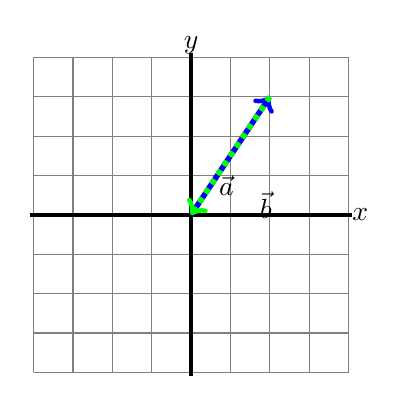
\begin{tikzpicture}[scale=0.5]

\draw[step=1.0,gray,thin] (-4,-4) grid (4,4);
\draw[black, line width=0.05 cm] (-4.1,0) -- (4.1,0);
\draw[black, line width=0.05 cm] (0,-4.1) -- (0,4.1);
\node at (0,4.3) {$y$};
\node at (4.3,0) {$x$};

\node at (0.9,0.75) {$\vec{a}$};
\draw[blue, line width=0.07 cm,->] (0,0) -- (2,3);

\node at (1.9,0.25) {$\vec{b}$};
\draw[green, line width=0.07 cm, ->,dotted] (2,3) -- (0,0);
\end{tikzpicture}
\end{center}
$\vec{a} + \vec{b}= \begin{pmatrix}
0 \\
0 
\end{pmatrix}$ This vector is zero.
\Question Vector addition\\
\subQuestion Draw the vectors $\vec{c} = \begin{pmatrix}
1 \\
1 
\end{pmatrix}$ and $\vec{d} = \begin{pmatrix}
-2 \\
3 
\end{pmatrix}$
\begin{center}

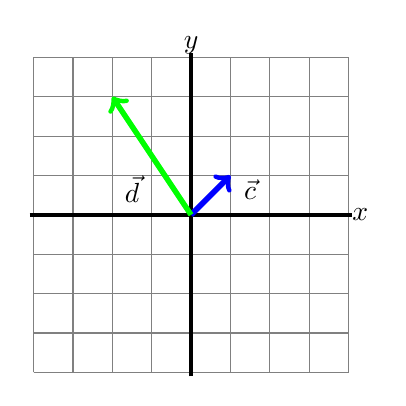
\begin{tikzpicture}[scale=0.5]

\draw[step=1.0,gray,thin] (-4,-4) grid (4,4);
\draw[black, line width=0.05 cm] (-4.1,0) -- (4.1,0);
\draw[black, line width=0.05 cm] (0,-4.1) -- (0,4.1);
\node at (0,4.3) {$y$};
\node at (4.3,0) {$x$};

\node at (1.5,0.65) {$\vec{c}$};
\draw[blue, line width=0.07 cm,->] (0,0) -- (1,1);

\node at (-1.5,0.65) {$\vec{d}$};
\draw[green, line width=0.07 cm, ->] (0,0) -- (-2,3);
\end{tikzpicture}
\end{center}
\subQuestion Draw the vector $\vec{i}=\vec{c}-\vec{d}$ and then the vector $\vec{f}=\vec{d}-\vec{c}$. Give the coordinates for both vectors. Any comments?
\begin{center}

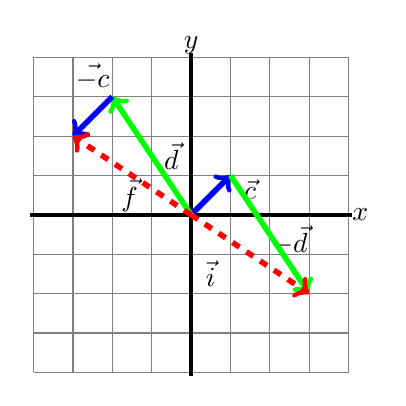
\begin{tikzpicture}[scale=0.5]

\draw[step=1.0,gray,thin] (-4,-4) grid (4,4);
\draw[black, line width=0.05 cm] (-4.1,0) -- (4.1,0);
\draw[black, line width=0.05 cm] (0,-4.1) -- (0,4.1);
\node at (0,4.3) {$y$};
\node at (4.3,0) {$x$};

\node at (1.5,0.65) {$\vec{c}$};
\draw[blue, line width=0.07 cm,->] (0,0) -- (1,1);

\node at (2.5,-0.65) {$-\vec{d}$};
\draw[green, line width=0.07 cm, ->] (1,1) -- (3,-2);

\node at (0.5,-1.5) {$\vec{i}$};
\draw[red, line width=0.07 cm, ->, dashed] (0,0) -- (3,-2);

\node at (-0.5,1.5) {$\vec{d}$};
\draw[green, line width=0.07 cm, ->] (0,0) -- (-2,3);

\node at (-2.5,3.5) {$\vec{-c}$};
\draw[blue, line width=0.07 cm,->] (-2,3) -- (-3,2);

\node at (-1.56,0.5) {$\vec{f}$};
\draw[red, line width=0.07 cm, ->, dashed] (0,0) -- (-3,2);

\end{tikzpicture}
\end{center}
$\vec{i} = \begin{pmatrix}
3 \\
-2 
\end{pmatrix}$ and $\vec{f} = \begin{pmatrix}
-3 \\
2 
\end{pmatrix}$. Both vectors are of the same length but go in the opposite directions. Although the order in which you add vectors does not affect the answer, the order in which you substract vectors matter. It is the same with scalars: $6+4=10$ and $4+6=10$ but $6-4=2$ and $4-6=-2$.  
\subQuestion Find the magnitude of $\vec{i}$, ($|\vec{i}|$).
\begin{eqnarray}
|\vec{i}|&=&\sqrt{i^2_x+i^2_y}\\
&=&\sqrt{3^2+(-2)^2}\\
&=&\sqrt{13}
\end{eqnarray}
\Question Vector multiplication
\subQuestion Draw $\vec{g} = \begin{pmatrix}
2 \\
4 
\end{pmatrix}$ 
\subQuestion Draw $2\vec{g}$ and give the coordinates of that new vector.
\begin{center}

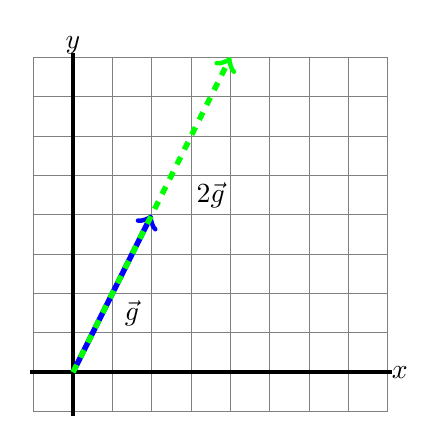
\begin{tikzpicture}[scale=0.5]

\draw[step=1.0,gray,thin] (-1,-1) grid (8,8);
\draw[black, line width=0.05 cm] (-1.1,0) -- (8.1,0);
\draw[black, line width=0.05 cm] (0,-1.1) -- (0,8.1);
\node at (0,8.3) {$y$};
\node at (8.3,0) {$x$};

\node at (1.5,1.5) {$\vec{g}$};
\draw[blue, line width=0.07 cm,->] (0,0) -- (2,4);

\node at (3.5,4.5) {$2 \vec{g}$};
\draw[green, line width=0.07 cm, ->, dashed] (0,0) -- (4,8);

\end{tikzpicture}
\end{center}
\Question Multiple dimensional vectors\\
\subQuestion What is the dimension of the following vector $\vec{h} = \begin{pmatrix}
2 \\
3 \\
-4\\
-6
\end{pmatrix}$ ?\\
This vector has four dimension
\subQuestion What are the coordinates of $5\vec{h}$?
\begin{equation}
5\vec{h} = \begin{pmatrix}
5\cdot 2 \\
5\cdot 3 \\
5\cdot -4\\
5\cdot -6
\end{pmatrix}
 = \begin{pmatrix}
10 \\
15 \\
-20\\
-30
\end{pmatrix} 
\end{equation}
\Question Basis vectors
\subQuestion In a two dimensional space, give the coordinates of the basis vectors in the first dimension ($\vec{e}_x$) and in the second dimension ($\vec{e}_y$)?\\
$\vec{e}_x = \begin{pmatrix}
1 \\
0 
\end{pmatrix}$ and $\vec{e}_y = \begin{pmatrix}
0 \\
1 
\end{pmatrix}$
\subQuestion What is special about these vectors?\\
These vectors are special because they have a length of 1 and point along one of the axis. They are used as reference.  

\end{Answer}

%%%%%%%%%%%%%%%%%%%%%%%%%%% MATRIcES %%%%%%%%%%%%%%%%%%%%%%%%%%%%%%%%%%%
\section{Vector Transformations}
\subsection{Graphically}\label{sec:linal:mat:gr}
So far we have been concerned with vectors: what they are and what happens when they are combined. We will now deal with linear transformations of vectors. That is instead of vectors themselves we look at operations that can change vectors. In general we will denote such transformations with a capital letter. When we have a transformation called $A$, then $A\vec{v}$ is the $\vec{v}$ transformed by $A$. To give you an idea we will now discuss 5 examples of transformations of a 2 dimensional vector.
\begin{enumerate}
\item \textbf{Nothing} The simplest thing that can happen is nothing. The vector $\vec{v}$ just remains $\vec{v}$. This is what we call \textbf{the identity transformation}.
\item \textbf{Rotation} A very common transformation is a rotation. Let us write $R_\theta$ for a rotation of $\theta$ degrees counter clockwise. Below two examples are shown: one for a rotation of $120^\circ$ and one for a rotation of $90^\circ$.
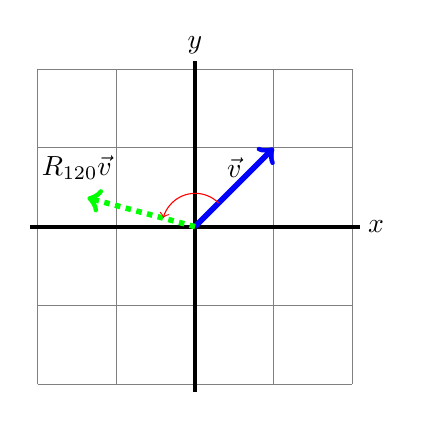
\begin{tikzpicture}
\draw[step=1.0,gray,thin] (-2,-2) grid (2,2);
\draw[black, line width=0.05 cm] (-2.1,0) -- (2.1,0);
\draw[black, line width=0.05 cm] (0,-2.1) -- (0,2.1);
\node at (0,2.3) {$y$};
\node at (2.3,0) {$x$};

\node at (0.5,0.75) {$\vec{v}$};
\draw[blue, line width=0.07 cm,->] (0,0) -- (1,1);
\draw[green, line width=0.07 cm, ->,dotted,rotate=120] (0,0) -- (1,1);
\node at (-1.5,0.75) {$R_{120}\vec{v}$};
 \draw[red,->]  (0.3,0.3) arc (45:165:0.42);

\end{tikzpicture}
\hspace{1cm}
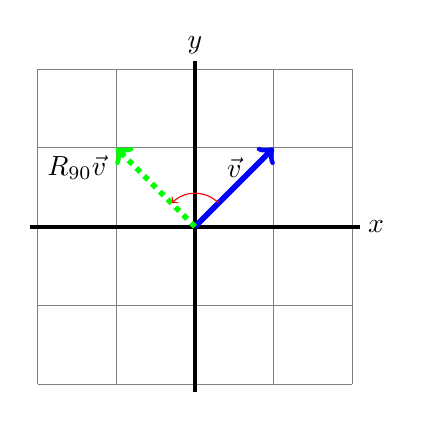
\begin{tikzpicture}
\draw[step=1.0,gray,thin] (-2,-2) grid (2,2);
\draw[black, line width=0.05 cm] (-2.1,0) -- (2.1,0);
\draw[black, line width=0.05 cm] (0,-2.1) -- (0,2.1);
\node at (0,2.3) {$y$};
\node at (2.3,0) {$x$};

\node at (0.5,0.75) {$\vec{v}$};
\draw[blue, line width=0.07 cm,->] (0,0) -- (1,1);
\draw[green, line width=0.07 cm, ->,dotted,rotate=90] (0,0) -- (1,1);
\node at (-1.5,0.75) {$R_{90}\vec{v}$};
 \draw[red,->]  (0.3,0.3) arc (45:135:0.42);
\end{tikzpicture}
\item \textbf{Mirror image} The next transformation is mirroring a vector with respect to a line. Below we illustrate this for (left) mirroring the vector with respect to the y-axis and (right) for mirroring the vector with respect to the x-axis. Mirroring can also be done with respect to other lines.
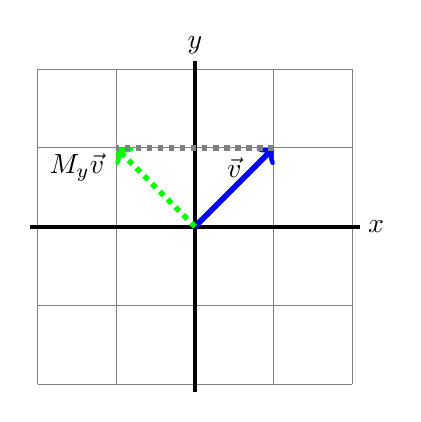
\begin{tikzpicture}
\draw[step=1.0,gray,thin] (-2,-2) grid (2,2);
\draw[black, line width=0.05 cm] (-2.1,0) -- (2.1,0);
\draw[black, line width=0.05 cm] (0,-2.1) -- (0,2.1);
\node at (0,2.3) {$y$};
\node at (2.3,0) {$x$};

\node at (0.5,0.75) {$\vec{v}$};
\draw[blue, line width=0.07 cm,->] (0,0) -- (1,1);
\draw[green, line width=0.07 cm, ->,dotted] (0,0) -- (-1,1);
\draw[gray, line width=0.07 cm,dotted] (1,1) -- (-1,1);
\node at (-1.5,0.75) {$M_y\vec{v}$};

\end{tikzpicture}
\hspace{1cm}
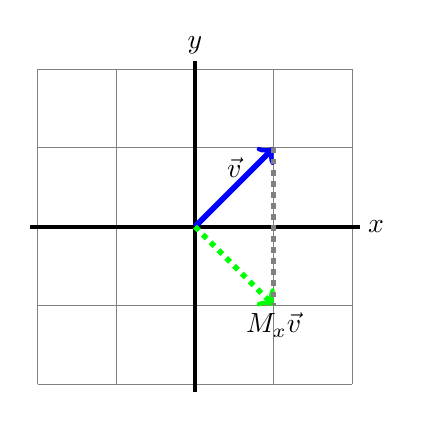
\begin{tikzpicture}
\draw[step=1.0,gray,thin] (-2,-2) grid (2,2);
\draw[black, line width=0.05 cm] (-2.1,0) -- (2.1,0);
\draw[black, line width=0.05 cm] (0,-2.1) -- (0,2.1);
\node at (0,2.3) {$y$};
\node at (2.3,0) {$x$};

\node at (0.5,0.75) {$\vec{v}$};
\draw[blue, line width=0.07 cm,->] (0,0) -- (1,1);
\draw[green, line width=0.07 cm, ->,dotted] (0,0) -- (1,-1);
\draw[gray, line width=0.07 cm,dotted] (1,1) -- (1,-1);
\node at (1,-1.25) {$M_x\vec{v}$};


\end{tikzpicture}
\item \textbf{Scaling} In the previous section we discussed multiplying a vector by a scalar. In this case both components of the vector would scale exactly the same. Instead it is also possible to scale the components separately, we could for example multiply the x-component by 1.5 and the y-component by 0.5. Let us call that transformation $S_{1.5,0.5}$. Below are two graphical examples of such a transformation.

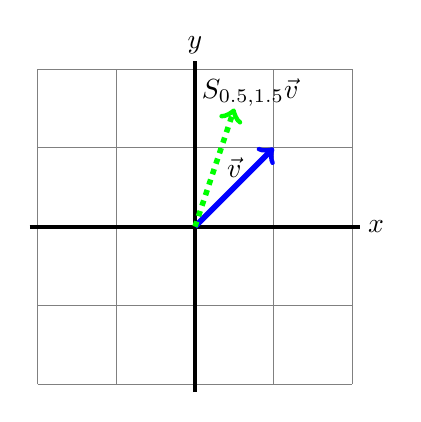
\begin{tikzpicture}
\draw[step=1.0,gray,thin] (-2,-2) grid (2,2);
\draw[black, line width=0.05 cm] (-2.1,0) -- (2.1,0);
\draw[black, line width=0.05 cm] (0,-2.1) -- (0,2.1);
\node at (0,2.3) {$y$};
\node at (2.3,0) {$x$};

\node at (0.5,0.75) {$\vec{v}$};
\draw[blue, line width=0.07 cm,->] (0,0) -- (1,1);
\draw[green, line width=0.07 cm, ->,dotted] (0,0) -- (0.5,1.5);
\node at (0.7,1.7) {$S_{0.5,1.5}\vec{v}$};

\end{tikzpicture}
\hspace{1cm}
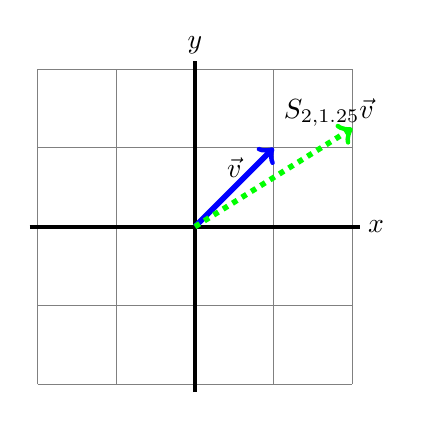
\begin{tikzpicture}
\draw[step=1.0,gray,thin] (-2,-2) grid (2,2);
\draw[black, line width=0.05 cm] (-2.1,0) -- (2.1,0);
\draw[black, line width=0.05 cm] (0,-2.1) -- (0,2.1);
\node at (0,2.3) {$y$};
\node at (2.3,0) {$x$};

\node at (0.5,0.75) {$\vec{v}$};
\draw[blue, line width=0.07 cm,->] (0,0) -- (1,1);
\draw[green, line width=0.07 cm, ->,dotted] (0,0) -- (2,1.25);
\node at (1.7,1.45) {$S_{2,1.25}\vec{v}$};


\end{tikzpicture}
\item \textbf{Projection} The last transformation we will treat here is the projection. This transformation simply isolates a part of the vector, for example the part of the vector that is along the x-axis ($P_x$) or the part that lies along the y-axis ($P_y$). Of course projections can also be made on other lines, but in the following figures for simplicity we will show projections on the x-axis and on the y-axis.

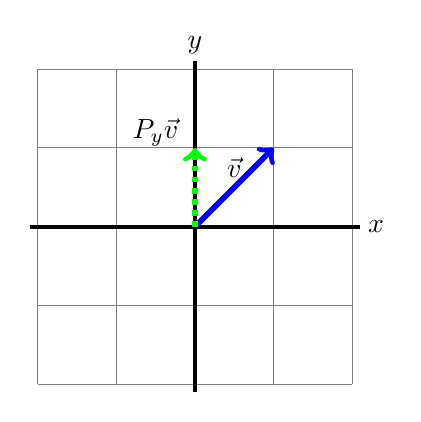
\begin{tikzpicture}
\draw[step=1.0,gray,thin] (-2,-2) grid (2,2);
\draw[black, line width=0.05 cm] (-2.1,0) -- (2.1,0);
\draw[black, line width=0.05 cm] (0,-2.1) -- (0,2.1);
\node at (0,2.3) {$y$};
\node at (2.3,0) {$x$};

\node at (0.5,0.75) {$\vec{v}$};
\draw[blue, line width=0.07 cm,->] (0,0) -- (1,1);
\draw[green, line width=0.07 cm, ->,dotted] (0,0) -- (0,1);
\node at (-0.5,1.2) {$P_y\vec{v}$};

\end{tikzpicture}
\hspace{1cm}
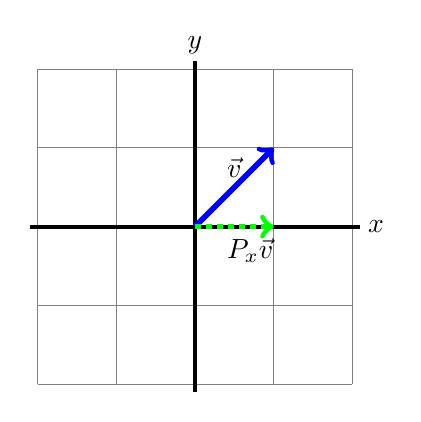
\begin{tikzpicture}
\draw[step=1.0,gray,thin] (-2,-2) grid (2,2);
\draw[black, line width=0.05 cm] (-2.1,0) -- (2.1,0);
\draw[black, line width=0.05 cm] (0,-2.1) -- (0,2.1);
\node at (0,2.3) {$y$};
\node at (2.3,0) {$x$};

\node at (0.5,0.75) {$\vec{v}$};
\draw[blue, line width=0.07 cm,->] (0,0) -- (1,1);
\draw[green, line width=0.07 cm, ->,dotted] (0,0) -- (1,0);
\node at (0.7,-0.3) {$P_x\vec{v}$};


\end{tikzpicture}
\end{enumerate}
\subsection{With numbers}
The type of transformations that we are discussing are the so-called linear transformations. The nice property of these transformations is that when you add up two vectors and then perform the transformation on the sum of these vectors, it gives exactly the same result as first performing the transformation on the separate vectors and then adding up these transformed vectors. In an equation this is:
\begin{equation}
A(\vec{u} + \vec{v}) = A\vec{u} + A\vec{v}
\label{optellen}
\end{equation}
Say that we want to know what happens to $\vec{v}$ when it is transformed by $A$. What information do we need to make sure we are always able to find the result of the transformation? To answer this question we first write our vector in terms of the basis vectors:
\begin{equation}
\vec{v} = \begin{pmatrix} v_x \\ v_y \end{pmatrix} = \begin{pmatrix} v_x \\ 0 \end{pmatrix} + \begin{pmatrix} 0 \\v_y \end{pmatrix} = v_x \begin{pmatrix} 1 \\ 0 \end{pmatrix} + v_y \begin{pmatrix} 0 \\ 1 \end{pmatrix}
\end{equation}
We now use this way of writing $\vec{v}$ together with equation \ref{optellen} and we find:
\begin{equation}
A\vec{v}  =  A v_x \begin{pmatrix} 1 \\ 0 \end{pmatrix} + A v_y \begin{pmatrix} 0 \\ 1 \end{pmatrix}
\label{tofu}
\end{equation}
In this equation $v_x$ and $v_y$ are not vectors but scalars. In general it is the case that the order in which a matrix $A$ and a scalar $a$ are multiplied does not matter:
\begin{equation}
A a = a A
\end{equation}
Using this we can write equation \ref{tofu} as follows:
\begin{equation}
A\vec{v}  =  v_x A \begin{pmatrix} 1 \\ 0 \end{pmatrix} + v_y A \begin{pmatrix} 0 \\ 1 \end{pmatrix}
\label{mateqnkip}
\end{equation}
What we have found is an important result: \textbf{in order to find out how any vector in 2 dimensional space is transformed by a linear transformation $A$, we only have to know how $A$ transforms the basis vectors $\vec{e}_x$ and $\vec{e}_y$}.

\subsection{Matrices}
Usually the information in equation \ref{mateqnkip} is written as a matrix, the columns of this matrix describe how each of the basis vectors look like after the transformation. That is, if we know that:
\begin{align}
A\begin{pmatrix} 1\\0\end{pmatrix} &= \begin{pmatrix} a_{1,1}\\a_{1,2}\end{pmatrix}\\[1.5em]
A\begin{pmatrix} 0\\1\end{pmatrix} &= \begin{pmatrix} a_{2,1}\\a_{2,2}\end{pmatrix}
\end{align}
We summarise this information by putting all the relevant information together and we write:
\begin{equation}
A = \begin{pmatrix} a_{1,1} & a_{1,2}\\ a_{2,1} & a_{2,2}\end{pmatrix}
\end{equation}
In this notation $a_{i,j}$ is simply a scalar that tells what the value is of the $i^{th}$ coordinate of the $j^{th}$ basisvector after the transformation. For example $a_{2,1}$ is the value of the second coordinate (the y-coordinate) of the transformed first basisvector.
\begin{mdframed}
In the matrix notation the element $a_{i,j}$ always refers to the element in row $i$ and column $j$. An easy way to remember that the first index refers to the row and the second to the column is by remembering that in Roman Catholic R also comes before C.
\end{mdframed}

\subsection{Examples}
We will now discuss the matrices for the 2 dimensional examples in section \ref{sec:linal:mat:gr}:
\begin{enumerate}
\item \textbf{Nothing} If nothing happens $\vec{e}_x$ remains $\vec{e}_x$ and $\vec{e}_y$ remains $\vec{e}_y$. This is what we call the identity matrix ($\mathbb{1}$).
\begin{equation*}
\mathbb{1} = \begin{pmatrix} 1 & 0 \\ 0 & 1 \end{pmatrix}
\end{equation*}
\item \textbf{Rotation}  We will describe only a rotation of $90^\circ$. The more general matrix for rotations is left as an exercise. If the vector $\vec{e}_x$ is rotated $90^\circ$ counterclockwise it will be the vector $\vec{e}_y$. If the vector $\vec{e}_y$ is rotated $90^\circ$ counterclockwise it will be the vector $-\vec{e}_x$, or as a matrix:
\begin{equation*}
R_{90}= \begin{pmatrix} 0 & -1\\ 1 & 0 \end{pmatrix}
\end{equation*}
\item \textbf{Mirror image} Again we consider only one example of a mirror image, two other mirror images are left as an exercise. Here we will consider mirroring a vector in the x-axis. This operation will not change $\vec{e}_x$, but it will change $\vec{e}_y$ into $-\vec{e}_y$, thus:
\begin{equation*}
M_x = \begin{pmatrix} 1 & 0 \\ 0 & -1 \end{pmatrix}
\end{equation*}
\item \textbf{Scaling} If we scale the x component of a vector with a factor $1.5$ and the y component with a factor $0.75$ the matrix describing this operation will look as follows:
\begin{equation*}
S_{1.5,0.75} = 
\begin{pmatrix}
1.5 & 0 \\ 0 & 0.75
\end{pmatrix}
\end{equation*}
\item \textbf{Projection} Finally we consider a projection on the x-axis. This operation will not change $\vec{e}_x$. It will however completely remove the y-component of the vector, that is $\vec{e}_y$ is transformed into 0.
\begin{equation*}
P_x = \begin{pmatrix} 1 & 0\\ 0 & 0 \end{pmatrix}
\end{equation*}
\end{enumerate}
\subsection{Matrix-Vector Multiplication}
In more dimensions everything is slightly more complicated (see next section), but for 2 dimensions it is not that bad:
\begin{equation}
A\vec{v} = \begin{pmatrix} a_{1,1} & a_{1,2} \\ a_{2,1} & a_{2,2} \end{pmatrix} \begin{pmatrix} v_x \\ v_y \end{pmatrix} = \begin{pmatrix} a_{1,1}v_x + a_{1,2} v_y \\ a_{2,1}v_x + a_{2,2}v_y \end{pmatrix}
\end{equation}
This equation describes how $\vec{v}$ will look like after it has been transformed by the matrix $A$.
\subsection{Larger dimensions}
So far we have just looked at transformations of 2 dimensional vectors. Of course 3 dimensional vectors can also be transformed by a matrix. In this case the matrix will have 3 rows and 3 columns. The first column describes what the first basis vector looks like after the transformation, the second column how the second will look like and the third what the third basis vector looks like. In general in 3 dimensional space:
\begin{equation}
A = \begin{pmatrix} a_{1,1} & a_{1,2} & a_{1,3} \\ a_{2,1} & a_{2,2} & a_{2,3} \\ a_{3,1} & a_{3,2} & a_{3,3} \end{pmatrix}
\end{equation}
\begin{equation}
A\vec{e}_i = \begin{pmatrix} a_{1,i} \\ a_{2,i} \\ a_{3,i} \end{pmatrix}
\end{equation}
In this last equation $i$ can be $1,2$ or $3$. Next we generalise matrices to even larger dimensions. If the dimension of the system is $N$, the previous equations look as follows:
\begin{equation}
A = \begin{pmatrix} a_{1,1} & a_{1,2} & \dots & a_{1,N} \\ a_{2,1} & a_{2,2} & \dots & a_{2,N} \\
\vdots & \vdots & \ddots & \vdots\\ a_{N,1} & a_{N,2} & \dots & a_{N,N} \end{pmatrix}
\end{equation}
\begin{equation}
A\vec{e}_i = \begin{pmatrix} a_{1,i} \\ a_{2,i} \\ \vdots \\ a_{N,i} \end{pmatrix}
\end{equation}
Now $i$ can be any integer in the range from $1$ to $N$.

\subsection{Matrix vector multiplication in larger dimensions}
In three dimensions a vector is transofrmed by a matrix as follows:
\begin{equation}
A\vec{v} = \begin{pmatrix} a_{1,1} & a_{1,2} & a_{1,3} \\ a_{2,1} & a_{2,2} & a_{2,3} \\ a_{3,1} & a_{3,2} & a_{3,3} \end{pmatrix} \begin{pmatrix} v_x \\ v_y \\ v_z \end{pmatrix} = \begin{pmatrix} a_{1,1}v_x + a_{1,2}v_y + a_{1,3}v_z \\ a_{2,1}v_x + a_{2,2}v_y + a_{2,3}v_z \\ a_{3,1}v_x + a_{3,2}v_y + a_{3,3}v_z\end{pmatrix}
\end{equation}
This is maybe a bit difficult to remember, so instead let us just look at how the first entry of the transformed vector is calculated:
\begin{equation}
A\vec{v} = 
\left( \begin{array}{ccc} 
\cline{1-3}
\multicolumn{1}{|c}{a_{1,1}} & a_{1,2} & \multicolumn{1}{c|}{a_{1,3}} \\ \cline{1-3} 
a_{2,1} & a_{2,2} & a_{2,3} \\ 
a_{3,1} & a_{3,2} & a_{3,3} 
\end{array} \right) 
\left(\begin{array}{|c|} \cline{1-1} v_x \\ v_y \\ v_z \\ \cline{1-1} \end{array}\right) = \left( \begin{array}{c} 
\cline{1-1} \multicolumn{1}{|c|}{a_{1,1}v_x + a_{1,2}v_y + a_{1,3}v_z} \\ \cline{1-1} a_{2,1}v_x + a_{2,2}v_y + a_{2,3}v_z \\ a_{3,1}v_x + a_{3,2}v_y + a_{3,3}v_z\end{array} \right)
\end{equation}
We take the first row of the matrix and multiply this number by the first entry of $\vec{v}$. To this we add the product of the second entry of the first row of the matrix and the second entry of $\vec{v}$. When we also add the product of the third entry of the first row of the matrix and the third entry of $\vec{v}$, this total sum gives us the first entry of the transformed vector. To get the second entry, we repeat the whole process, but instead of the first row of the matrix we now use the second row of the matrix.
\begin{equation}
A\vec{v} = 
\left( \begin{array}{ccc} 
a_{1,1} & a_{1,2} & a_{1,3} \\ \cline{1-3} 
\multicolumn{1}{|c}{a_{2,1}} & a_{2,2} &\multicolumn{1}{c|}{a_{2,3}} \\ \cline{1-3}
a_{3,1} & a_{3,2} & a_{3,3} 
\end{array} \right) 
\left(\begin{array}{|c|} \cline{1-1} v_x \\ v_y \\ v_z \\ \cline{1-1} \end{array}\right) = \left( \begin{array}{c} 
a_{1,1}v_x + a_{1,2}v_y + a_{1,3}v_z \\ \cline{1-1} \multicolumn{1}{|c|}{a_{2,1}v_x + a_{2,2}v_y + a_{2,3}v_z} \\ \cline{1-1} a_{3,1}v_x + a_{3,2}v_y + a_{3,3}v_z\end{array} \right)
\end{equation}
We will now write this procedure down as an equation. If $\vec{u}$ is the transformed vector ($\vec{u}=A\vec{v}$) then, for the $i^{th}$ entry of $\vec{u}$:
\begin{equation}
u_i = \sum_{j=1}^3 a_{i,j} v_j 
\end{equation}
In this notation the $\Sigma$ mean summation: it adds up all arguments that it has in it for which $j$ is between 1 and 3 (these limits are given below and above the $\Sigma$-sign). For example:
\begin{equation}
\sum_{j=1}^3 a_{1,j} = a_{1,1} + a_{1,2} + a_{1,3}
\end{equation}
In even larger dimensions, multiplying a vector by a matrix works in a similar manner, we just extend the number of values that $j$ can have. If we have $N$ dimensions and $\vec{u}=A\vec{v}$, then:
\begin{equation}
u_i = \sum_{j=1}^N a_{i,j} v_j 
\end{equation}
\subsection{The order of matrix multiplications}
You probably remember that when we multiply two scalars, the order does not
matter:
\begin{equation}
3 \cdot 4= 4 \cdot 3
\end{equation}
For matrices this is unfortunately not always true: in general the order of the
multiplication does matter.\\
\begin{mdframed}[backgroundcolor=exampcol]
\textbf{Graphical example}\\
Let us consider the vector $\vec{v}=\begin{pmatrix} 1\\ 1\end{pmatrix}$:
\begin{center}
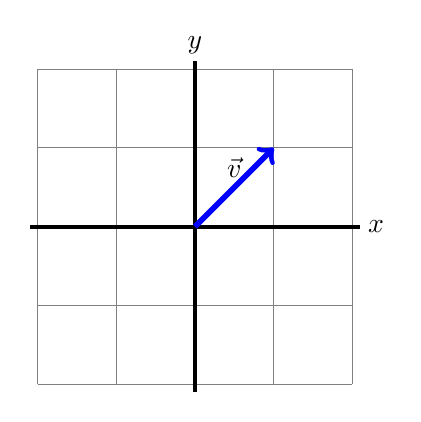
\begin{tikzpicture}
\draw[step=1.0,gray,thin] (-2,-2) grid (2,2);
\draw[black, line width=0.05 cm] (-2.1,0) -- (2.1,0);
\draw[black, line width=0.05 cm] (0,-2.1) -- (0,2.1);
\node at (0,2.3) {$y$};
\node at (2.3,0) {$x$};

\node at (0.5,0.75) {$\vec{v}$};
\draw[blue, line width=0.07 cm,->] (0,0) -- (1,1);

\end{tikzpicture}
\end{center}
If we now first rotates this vector $90\,^{\circ}$ counterclockwise ($R_{90}$) and then mirror the resulting vector in the $x-axis$ ($M_x$), we find the following:

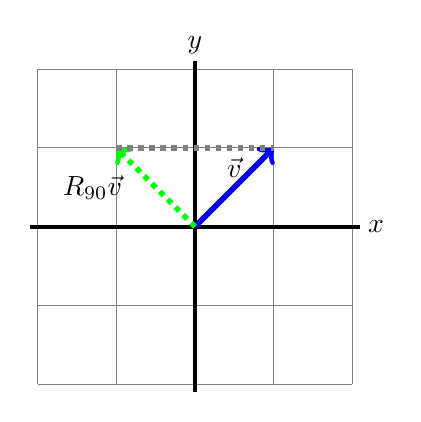
\begin{tikzpicture}
\draw[step=1.0,gray,thin] (-2,-2) grid (2,2);
\draw[black, line width=0.05 cm] (-2.1,0) -- (2.1,0);
\draw[black, line width=0.05 cm] (0,-2.1) -- (0,2.1);
\node at (0,2.3) {$y$};
\node at (2.3,0) {$x$};

\node at (0.5,0.75) {$\vec{v}$};
\draw[blue, line width=0.07 cm,->] (0,0) -- (1,1);
\node at (-1.3,0.5) {$R_{90}\vec{v}$};
\draw[green, line width=0.07 cm,->, dotted] (0,0) -- (-1,1);
\draw[gray, line width=0.07 cm,-, dotted] (-1,1) -- (1,1);
\end{tikzpicture}
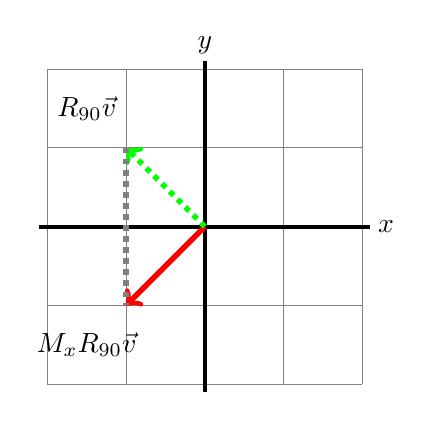
\begin{tikzpicture}
\draw[step=1.0,gray,thin] (-2,-2) grid (2,2);
\draw[black, line width=0.05 cm] (-2.1,0) -- (2.1,0);
\draw[black, line width=0.05 cm] (0,-2.1) -- (0,2.1);
\node at (0,2.3) {$y$};
\node at (2.3,0) {$x$};

\node at (-1.5,-1.5) {$M_xR_{90}\vec{v}$};
\draw[red, line width=0.07 cm,->] (0,0) -- (-1,-1);
\node at (-1.5,1.5) {$R_{90}\vec{v}$};
\draw[green, line width=0.07 cm,->, dotted] (0,0) -- (-1,1);
\draw[gray, line width=0.07 cm,-, dotted] (-1,1) -- (-1,-1);
\end{tikzpicture}\\
If instead we mirror the verctor in the $x-axis$ and then rotate it $90\,^{\circ}$ counterclockwise, we find the following:\\
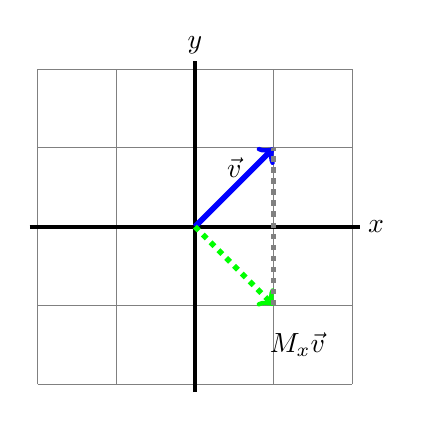
\begin{tikzpicture}
\draw[step=1.0,gray,thin] (-2,-2) grid (2,2);
\draw[black, line width=0.05 cm] (-2.1,0) -- (2.1,0);
\draw[black, line width=0.05 cm] (0,-2.1) -- (0,2.1);
\node at (0,2.3) {$y$};
\node at (2.3,0) {$x$};

\node at (0.5,0.75) {$\vec{v}$};
\draw[blue, line width=0.07 cm,->] (0,0) -- (1,1);
\node at (1.3,-1.5) {$M_x\vec{v}$};
\draw[green, line width=0.07 cm,->, dotted] (0,0) -- (1,-1);
\draw[gray, line width=0.07 cm,-, dotted] (1,-1) -- (1,1);
\end{tikzpicture}
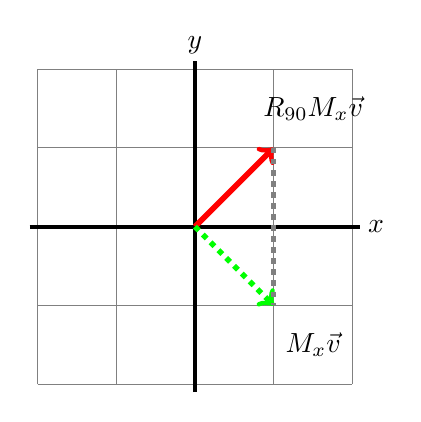
\begin{tikzpicture}
\draw[step=1.0,gray,thin] (-2,-2) grid (2,2);
\draw[black, line width=0.05 cm] (-2.1,0) -- (2.1,0);
\draw[black, line width=0.05 cm] (0,-2.1) -- (0,2.1);
\node at (0,2.3) {$y$};
\node at (2.3,0) {$x$};

\node at (1.5,1.5) {$R_{90}M_x\vec{v}$};
\draw[red, line width=0.07 cm,->] (0,0) -- (1,1);
\node at (1.5,-1.5) {$M_x\vec{v}$};
\draw[green, line width=0.07 cm,->, dotted] (0,0) -- (1,-1);
\draw[gray, line width=0.07 cm,-, dotted] (1,1) -- (1,-1);
\end{tikzpicture}\\
The final vectors (in red) point in opposite directions: the order in which we perform the transformation thus has an influence on the final outcome.\\
\textbf{Numerical Example}\\
Let us now consider a three dimensional vector $\vec{v}$:
\begin{equation*}
\vec{v}=\begin{pmatrix} 1\\2\\1\end{pmatrix} 
\end{equation*}
Next, we define two matrices $A$ and $B$:
\begin{align*}
A&=\begin{pmatrix} 0 & 2 & 3\\0.5 & 0 & 0\\0 & 0.5 & 0.5 \end{pmatrix} &
B&=\begin{pmatrix} 0 & 1 & 2\\0.8 & 0 & 0\\0 & 0.8 & 0.4 \end{pmatrix} 
\end{align*}
First we consider $AB\vec{v}$, this is the same as $A(B\vec{v})$. We calculate $B\vec{v}$:
\begin{equation*}
B\vec{v}=\begin{pmatrix} 0 & 1 & 2\\0.8 & 0 & 0\\0 & 0.8 & 0.4 \end{pmatrix} \begin{pmatrix} 1\\2\\1\end{pmatrix} = \begin{pmatrix} 0\cdot 1 + 1\cdot 2 + 2 \cdot 1\\0.8 \cdot 1 + 0\cdot 2 + 0 \cdot 1\\0 \cdot 1 + 0.8 \cdot 2 +0.4 \cdot 1\end{pmatrix}=\begin{pmatrix}4\\0.8\\2\end{pmatrix}
\end{equation*}
Now we apply matrix $A$:
\begin{eqnarray*}
AB\vec{v}&=&A(B\vec{v})=\begin{pmatrix} 0 & 2 & 3\\0.5 & 0 & 0\\0 & 0.5 & 0.5 \end{pmatrix}\begin{pmatrix}4\\0.8\\2\end{pmatrix}= \begin{pmatrix}0 \cdot 4+2 \cdot 0.8+3\cdot2\\0.5\cdot 4 + 0\cdot 0.8 + 0 \cdot 2\\0\cdot 3+ 0.5\cdot 0.8+0.5 \cdot 2\end{pmatrix}\\
&=&\begin{pmatrix}7.6\\2\\1.4\end{pmatrix}
\end{eqnarray*}
If we reverse the order, we nd (this time we left out the middle step, if
you have time, please do verify the equations below):
\begin{equation*}
A\vec{v}=\begin{pmatrix} 0 & 2 & 3\\0.5 & 0 & 0\\0 & 0.5 & 0.5 \end{pmatrix}\begin{pmatrix} 1\\2\\1\end{pmatrix}=\begin{pmatrix} 7\\0.5\\1.5\end{pmatrix}
\end{equation*}
And now:
\begin{equation*}
BA\vec{v}=B(A\vec{v})=\begin{pmatrix} 0 & 1 & 2\\0.8 & 0 & 0\\0 & 0.8 & 0.4 \end{pmatrix}\begin{pmatrix} 7\\0.5\\1.5\end{pmatrix}=\begin{pmatrix} 3.5\\5.6\\1\end{pmatrix}
\end{equation*}
So in this case we also note that $BA\vec{v}$ is different from $AB\vec{v}$. The order in which we apply the matrices thus makes a dierence in the final outcome.
\end{mdframed}
\subsection{Exercises}

\begin{Exercise}[label=linalg:mat:8,title=A general matrix for scaling,difficulty=1]
\Question Graphical exercise 
\subQuestion Draw $A\vec{u}$, where $A\vec{u}=\begin{pmatrix}2&0\\0&-2\end{pmatrix}\begin{pmatrix}1\\1\end{pmatrix}$
\subQuestion Draw $B\vec{u}$, where $B\vec{u}=\begin{pmatrix}3&0\\0&3\end{pmatrix}\begin{pmatrix}1\\1\end{pmatrix}$
\Question Caluculate:
\subQuestion $A\vec{u}=\begin{pmatrix}1&3\\5&7\end{pmatrix}\begin{pmatrix}7\\7\end{pmatrix}$
\subQuestion $B\vec{v}=\begin{pmatrix}2&4&6\\1&3&5\\0&0&1\end{pmatrix}\begin{pmatrix}1\\1\\1\end{pmatrix}$
\subQuestion $C\vec{w}=\begin{pmatrix}1&-4\\-2&0\end{pmatrix}\begin{pmatrix}-5\\2\end{pmatrix}$
\subQuestion $D\vec{z}=\begin{pmatrix}3&3&0\\0&-8&0\\0&0&7\end{pmatrix}\begin{pmatrix}-5\\0\\-6\end{pmatrix}$
\end{Exercise}

\begin{Answer}[ref=linalg:mat:8]
\Question Graphical exercise 
\subQuestion Draw $A\vec{u}$, where $A\vec{u}=\begin{pmatrix}2&0\\0&-2\end{pmatrix}\begin{pmatrix}1\\1\end{pmatrix}$
\begin{center}
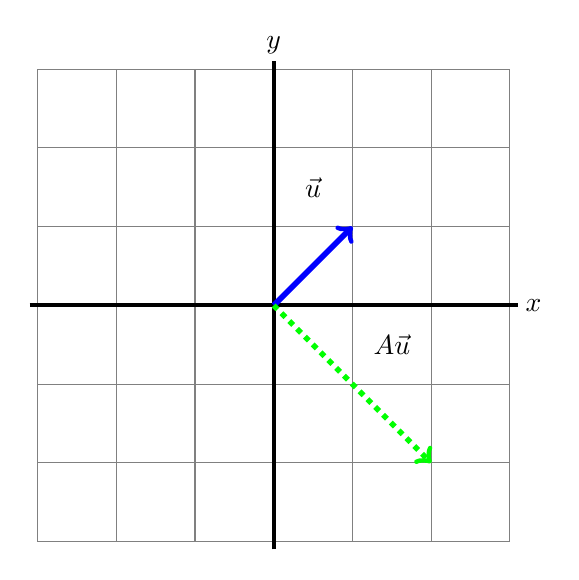
\begin{tikzpicture}
\draw[step=1.0,gray,thin] (-3,-3) grid (3,3);
\draw[black, line width=0.05 cm] (-3.1,0) -- (3.1,0);
\draw[black, line width=0.05 cm] (0,-3.1) -- (0,3.1);
\node at (0,3.3) {$y$};
\node at (3.3,0) {$x$};

\node at (0.5,1.5) {$\vec{u}$};
\draw[blue, line width=0.07 cm,->] (0,0) -- (1,1);
\node at (1.5,-0.5) {$A\vec{u}$};
\draw[green, line width=0.07 cm,->, dotted] (0,0) -- (2,-2);

\end{tikzpicture}\\
\end{center}
\subQuestion Draw $B\vec{u}$, where $B\vec{u}=\begin{pmatrix}3&0\\0&3\end{pmatrix}\begin{pmatrix}1\\1\end{pmatrix}$
\begin{center}
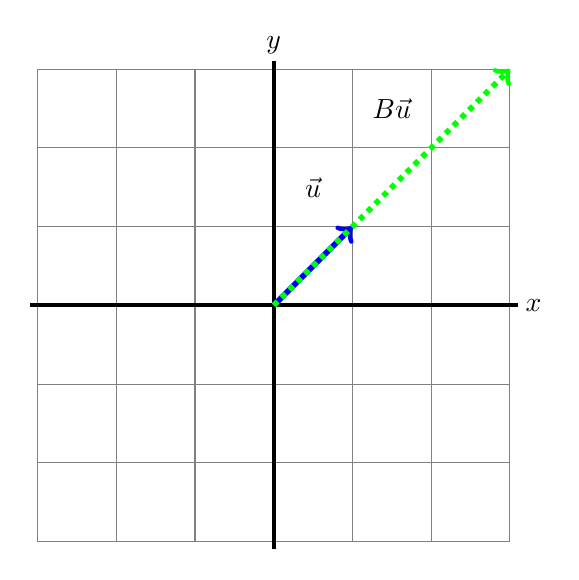
\begin{tikzpicture}
\draw[step=1.0,gray,thin] (-3,-3) grid (3,3);
\draw[black, line width=0.05 cm] (-3.1,0) -- (3.1,0);
\draw[black, line width=0.05 cm] (0,-3.1) -- (0,3.1);
\node at (0,3.3) {$y$};
\node at (3.3,0) {$x$};

\node at (0.5,1.5) {$\vec{u}$};
\draw[blue, line width=0.07 cm,->] (0,0) -- (1,1);
\node at (1.5,2.5) {$B\vec{u}$};
\draw[green, line width=0.07 cm,->, dotted] (0,0) -- (3,3);

\end{tikzpicture}\\
\end{center}

\Question Calculate:
\subQuestion $A\vec{u}=\begin{pmatrix}1&3\\5&7\end{pmatrix}\begin{pmatrix}7\\7\end{pmatrix}= \begin{pmatrix}2+12\\10+28\end{pmatrix}=\begin{pmatrix}14\\38\end{pmatrix}$
\subQuestion $B\vec{v}=\begin{pmatrix}2&4&6\\1&3&5\\0&0&1\end{pmatrix}\begin{pmatrix}1\\1\\1\end{pmatrix}=\begin{pmatrix}2+4+6\\1+3+5\\0+0+1\end{pmatrix}=\begin{pmatrix}12\\9\\1\end{pmatrix}$
\subQuestion $C\vec{w}=\begin{pmatrix}1&-4\\-2&0\end{pmatrix}\begin{pmatrix}-5\\2\end{pmatrix}=\begin{pmatrix}-5+(-8)\\10+0\end{pmatrix}=\begin{pmatrix}-13\\10\end{pmatrix}$
\subQuestion $D\vec{z}=\begin{pmatrix}3&3&0\\0&-8&0\\0&0&7\end{pmatrix}\begin{pmatrix}-5\\0\\-6\end{pmatrix}=\begin{pmatrix}-15+0+0\\0+0+0\\0+0+(-42)\end{pmatrix}=\begin{pmatrix}-15\\0\\-42\end{pmatrix}$
\end{Answer}

\begin{Exercise}[label=alba,title=Population ecology and matrices, difficulty=1]
Consider a population of wandering albatrosses. This year the population contains 20 juveniles, 16 sub-adults and 12 adults. We have been observing the population for a few years now and from these observations we expect the following to happen in the coming year:
\begin{itemize}
\item Of the juveniles 40\% will become sub-adults, 40\% will remain juveniles and 20\% die.
\item Of the sub-adults 50\% remain a sub-adult, 25\% become an adult and 25\% dies.
\item Of the current adults, 25\% give birth to 1 juvenile. Apart from that 25\% of the adults die and thus 75\% survive to next year
\end{itemize}
\Question Calculate how many juveniles, sub-adults and adults there will be next year.
\Question Calculate the following expression:
\begin{equation*}
\begin{pmatrix}0.4&0&0.25\\0.4&0.5&0\\0&0.25&0.75\end{pmatrix}\begin{pmatrix}20\\16\\12\end{pmatrix}
\end{equation*}
\Question How can the matrix in question 2 help you solve question 1?
\Question Good conditions
It turns out that the wind was very favourable this year and instead of
25\% of the adults, one third of the albatrosses gave birth to a juvenile.
Can you:
\subQuestion Correct the matrix in question 2 based on this information
\subQuestion Use this matrix to calculate how the population actually looks like after one year?
\end{Exercise}
\begin{Answer}[ref=alba]
\Question Calculate how many juveniles, sub-adults and adults there will be next year. 
\begin{itemize}
\item For the juveniles: 40\% of the current juveniles remain a juvenile, this is equal to $8$ juveniles. On top of that 25\% of the adults gives birth, this gives an additional $3$ juveniles. The total number of juveniles next year will thus be $11$. ($0.4 \cdot 20 + 0.25 \cdot 12 = 11$)
\item  for the sub-adults: 40\% of the juveniles will become a sub-adult, this gives $8$ sub-adults. On top of that 50\% of the current sub-adults will remain a sub-adult, this gives an additional $8$ sub-adults. In total there will thus be $16$ sub-adults next year. ($0.4 \cdot 20 + 0.5 \cdot 16 = 16$)
\item For the adults: 25\% of the current sub-adults will become an adult next year, this is equal to $4$ adults. On top of that 75\% of the current adults remain an adult, this gives an additional $9$ adults. In total there will thus be $13$ adults next year.($0.25\cdot 16+0.75 \cdot 12 = 13$)
\end{itemize}
\Question Evaluating a matrix multiplication
\begin{equation*}
\begin{pmatrix}0.4&0&0.25\\0.4&0.5&0\\0&0.25&0.75\end{pmatrix}\begin{pmatrix}20\\16\\12\end{pmatrix}=\begin{pmatrix}11\\16\\13\end{pmatrix}
\end{equation*}
\Question Relating question 1 to question 2\\
The vector in question $2$ corresponds to the current population size. From top to bottom the vector contains the number of juveniles, subadults and adults. In the matrix we see how the population changes. The first column tells us that 40\% of the current juveniles will stay juveniles and that another 40\% of the juveniles will become subadults. The second column shows how the subadults will develop (how many of them will remain subadults and how many will become adults.) Finally, the last column of the matrix show how much the adults contribute to the population the next year (25\% give birth to a young and apart from that 75\% of the adults survive the year and remain adults.) When we multiply the vector with the current population numbers by the matrix with all the transition chances, we get the vector with the population numbers for next year.
\Question Good conditions
\subQuestion The next matrix will look as follows:
\begin{equation*}
\begin{pmatrix}
0.4&0&0.333\\0.4&0.5&0\\0&0.25&0.75
\end{pmatrix}
\end{equation*}
\subQuestion Using matrix multiplication, we find:
\begin{equation*}
\begin{pmatrix}
0.4&0&0.333\\0.4&0.5&0\\0&0.25&0.75
\end{pmatrix}
\begin{pmatrix}
20\\16\\12
\end{pmatrix}=\begin{pmatrix}
12\\16\\13
\end{pmatrix}
\end{equation*}
That means that the following year there were 12 juveniles, 16 subadults and 13 adults. 

\end{Answer}
\section{Eigenvalues and eigenvectors}

\subsection{Graphically}
We have seen that matrices can alter both the length and the direction of a vector. However, for each matrix there are vectors which direction is not changed by the matrix. We call these eigenvectors of this matrix. Let us for example consider the matrix that multiplies the length of a vector by 2 and mirrors it in the x-axis:
\begin{equation}
A = \begin{pmatrix} 2 & 0 \\ 0 & -2 \end{pmatrix}
\end{equation}
Let us apply this matrix to the vector $\vec{v}$, which is such that the matrix does not change the direction of this vector:
\begin{center}
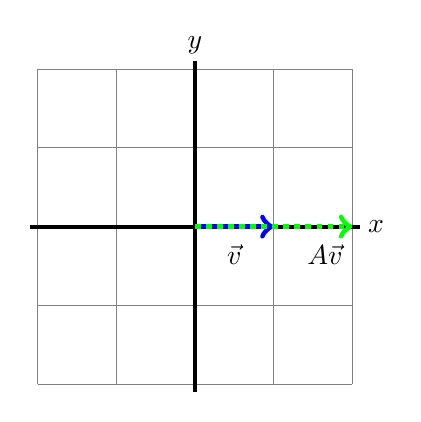
\begin{tikzpicture}
\draw[step=1.0,gray,thin] (-2,-2) grid (2,2);
\draw[black, line width=0.05 cm] (-2.1,0) -- (2.1,0);
\draw[black, line width=0.05 cm] (0,-2.1) -- (0,2.1);
\node at (0,2.3) {$y$};
\node at (2.3,0) {$x$};

\node at (0.5,-0.35) {$\vec{v}$};
\draw[blue, line width=0.07 cm,->] (0,0) -- (1,0);
\draw[green, line width=0.07 cm, ->,dotted] (0,0) -- (2,0);

\node at (1.65,-0.35) {$A \vec{v}$};


\end{tikzpicture}
\end{center}
\textbf{Because $A$ does not change the direction of the vector $\vec{v}$, we say that $\vec{v}$ is an eigenvector of $A$. $A$ does change the length of $\vec{v}$ by a factor $2$, therefore we say that the corresponding eigenvalue is $2$.} The matrix $A$ has a second eigenvector: $\vec{u}$. This one is a bit more difficult to see.
\begin{center}
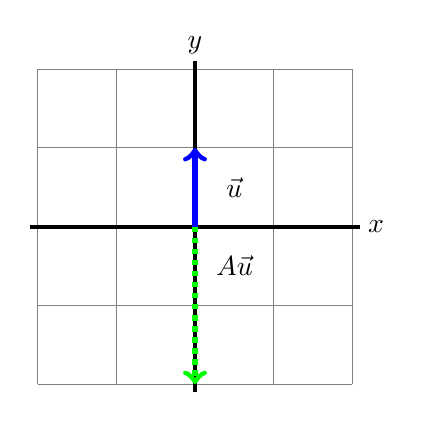
\begin{tikzpicture}
\draw[step=1.0,gray,thin] (-2,-2) grid (2,2);
\draw[black, line width=0.05 cm] (-2.1,0) -- (2.1,0);
\draw[black, line width=0.05 cm] (0,-2.1) -- (0,2.1);
\node at (0,2.3) {$y$};
\node at (2.3,0) {$x$};


\node at (0.5,0.5) {$\vec{u}$};
\draw[blue, line width=0.07 cm,->] (0,0) -- (0,1);
\draw[green, line width=0.07 cm, ->,dotted] (0,0) -- (0,-2);

\node at (0.5,-0.5) {$A \vec{u}$};

\end{tikzpicture}
\end{center}
Actually the direction of the vector did change: the new vector is pointing in the exact opposite direction as the original vector. Vectors for which this happens are also eigenvectors of $A$. The eigenvalue of corresponding to this eigenvector is $-2$. The minus sign indicates that the vector was inverted, the value of $2$ indicates that the length of the vector was doubled.

\subsection{With numbers}
Numerically it is a bit easier to define the eigenvectors. The eigenvectors are those vectors of a matrix that when the matrix is applied  on them, it is as if the vector is merely multiplied by a scalar instead of by a matrix. This scalar is the eigenvalue, which is usually denoted as $\lambda$.

Let us consider the example from the previous section: mirroring a vector in the x-axis. First we look at the effect of the matrix on the first eigenvector that we identified in the previous section ($\vec{v}$). From the grpah we can read that $\vec{v}=\begin{pmatrix}1\\0\end{pmatrix}$. So
\begin{equation}
A\vec{v} = \begin{pmatrix} 2 & 0 \\ 0 & -2 \end{pmatrix} \begin{pmatrix} 1 \\ 0 \end{pmatrix} = \begin{pmatrix} 2 \\ 0 \end{pmatrix} = 2\vec{v}
\end{equation}
We see that when $\vec{v}$ is transformed by $A$, this is the same effect as multiplying it with the scalar $2$. We have thus confirmed that $\vec{v}$ is an eigenvector. We can do the same for the second eigenvector. From the graph we can read that $\vec{u}=\begin{pmatrix}0\\1\end{pmatrix}$.
\begin{equation}
A\vec{u} = \begin{pmatrix} 2 & 0 \\ 0 & -2 \end{pmatrix} \begin{pmatrix} 0 \\ 1 \end{pmatrix} = \begin{pmatrix} 0 \\ -2 \end{pmatrix} = -2\vec{u}
\end{equation}
And so we see that also $\vec{u}$ is an eigenvector of $A$ and that this eigenvector has the eigenvalue $\lambda=-2$.
\subsection{Exercises}
\begin{Exercise}[label=eigen,title=Which of the two?, difficulty=1]
Below are four matirces, for each you can choose between two vectors. Choose the vector that is an eigenvector for that matrix and find the corresponding eigenvalue.
\begin{align*}
1.& \begin{pmatrix} 1&0.5\\0.5&2\end{pmatrix} & a)& \begin{pmatrix}0.38\\0.92 \end{pmatrix}& b)& \begin{pmatrix}0.17\\0.53 \end{pmatrix}\\
2.& \begin{pmatrix} 3&1.5\\-0.5&1\end{pmatrix} & a)& \begin{pmatrix}0.17\\0.53 \end{pmatrix}& b)& \begin{pmatrix}0.95\\-0.32 \end{pmatrix}\\
3.& \begin{pmatrix} 1&0&1.2\\0.5&0.8&0\\0&0.5&0.8\end{pmatrix} & a)& \begin{pmatrix}0.63\\0.27\\0.31 \end{pmatrix}& b)& \begin{pmatrix}0.78\\0.52\\0.35 \end{pmatrix}\\
4.& \begin{pmatrix} 1&0&0\\0&0&2\\0&3&0\end{pmatrix} & a)& \begin{pmatrix}0\\1\\0 \end{pmatrix}& b)& \begin{pmatrix}1\\0\\ 0\end{pmatrix}\\
\end{align*}
\end{Exercise}

\begin{Answer}[ref=eigen]
\textit{We have outlined the procedure to find the answer only for the first matrix. For the other matrices, the procesdure is exactly the same. For these matrices, on ly the correct answers are given.}
\begin{enumerate}
\item The correct answer is $a$.
\begin{equation*}
\begin{pmatrix} 1&0.5\\0.5&2\end{pmatrix} \begin{pmatrix}0.38\\0.92 \end{pmatrix} = \begin{pmatrix}0.84\\2.03 \end{pmatrix}\\
\end{equation*}
The x-component has increased with a factor $\frac{0.84}{0.38}\approx 2.21$ and the y-component has also increaser with a factor $\frac{2.03}{0.92}\approx 2.21$. We can thus write:
\begin{equation*}
\begin{pmatrix} 1&0.5\\0.5&2\end{pmatrix} \begin{pmatrix}0.38\\0.92 \end{pmatrix} =2.21 \begin{pmatrix}0.38\\0.92 \end{pmatrix}
\end{equation*}
Therefor $a$ is the correct answer and the corresponding eigenvalue is 2.21.
\item The correct answer is $b$, the corresponding eigenvalue is $2.5$.
\item The correct answer is $b$, the corresponding eigenvalue is $1.5$.
\item The correct answer is $b$, the corresponding eigenvalue is $1$.
\end{enumerate}
\end{Answer}

\begin{Exercise}[label=eigen2,title=Finding eigenvectors, difficulty=1]
Consider the following transformation that mirrors every vector in the line $x=y$ (we call this transformation $M_{xy}$): 
\begin{center}
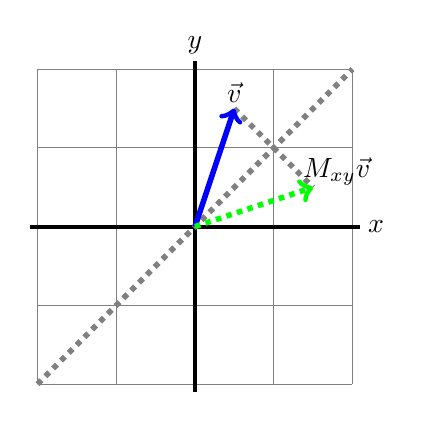
\begin{tikzpicture}
\draw[step=1.0,gray,thin] (-2,-2) grid (2,2);
\draw[black, line width=0.05 cm] (-2.1,0) -- (2.1,0);
\draw[black, line width=0.05 cm] (0,-2.1) -- (0,2.1);
\node at (0,2.3) {$y$};
\node at (2.3,0) {$x$};

\draw[gray, line width=0.07 cm, -,dotted] (-2,-2) -- (2,2);
\draw[gray, line width=0.07 cm, -,dotted] (0.5,1.5) -- (1.5,0.5);
\node at (0.5,1.7) {$\vec{v}$};
\draw[blue, line width=0.07 cm,->] (0,0) -- (0.5,1.5);
\draw[green, line width=0.07 cm, ->,dotted] (0,0) -- (1.5,0.5);

\node at (1.8,0.7) {$M_{xy} \vec{v}$};

\end{tikzpicture}
\end{center}
\Question What are the two eigenvectors for this transformation? What are the corresponding eigenvalues?
\Question Find the matrix that describes this transformation.
\Question Show with this matrix that the eigenvectors and eigenvalues that you found in question 1 are indeed correct.
\end{Exercise}

\begin{Answer}[ref=eigen2]
\Question The eigenvectors and eigenvalues\\
You have to see it; the vectors are $\vec{v}_1 = \begin{pmatrix}1\\1\end{pmatrix}$ with eigenvalue 1 and $\vec{v}_2 = \begin{pmatrix}-1\\1\end{pmatrix}$ with eigenvalue $-1$. All vectors that are a scalar times $\vec{v}_1$ or $\vec{v}_2$ are also eigenvectors.

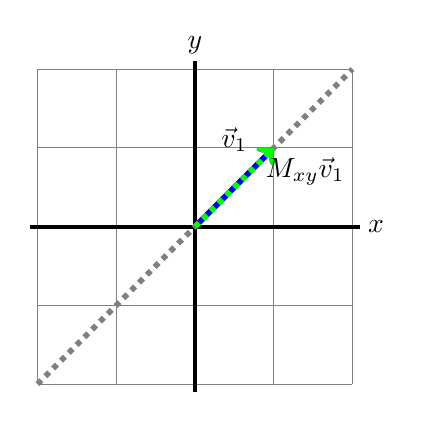
\begin{tikzpicture}
\draw[step=1.0,gray,thin] (-2,-2) grid (2,2);
\draw[black, line width=0.05 cm] (-2.1,0) -- (2.1,0);
\draw[black, line width=0.05 cm] (0,-2.1) -- (0,2.1);
\node at (0,2.3) {$y$};
\node at (2.3,0) {$x$};

\draw[gray, line width=0.07 cm, -,dotted] (-2,-2) -- (2,2);
\node at (0.5,1.1) {$\vec{v}_1$};
\draw[blue, line width=0.07 cm,->] (0,0) -- (1,1);
\draw[green, line width=0.07 cm, ->,dotted] (0,0) -- (1,1);

\node at (1.4,0.7) {$M_{xy} \vec{v}_1$};
\end{tikzpicture}
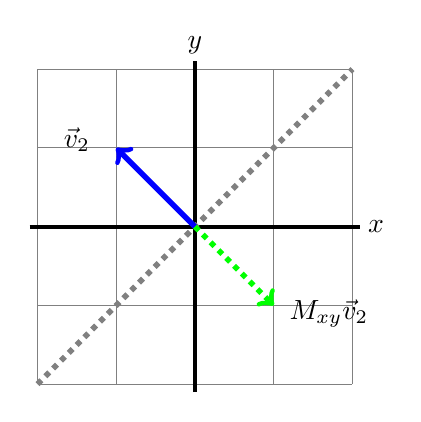
\begin{tikzpicture}
\draw[step=1.0,gray,thin] (-2,-2) grid (2,2);
\draw[black, line width=0.05 cm] (-2.1,0) -- (2.1,0);
\draw[black, line width=0.05 cm] (0,-2.1) -- (0,2.1);
\node at (0,2.3) {$y$};
\node at (2.3,0) {$x$};

\draw[gray, line width=0.07 cm, -,dotted] (-2,-2) -- (2,2);
\node at (-1.5,1.1) {$\vec{v}_2$};
\draw[blue, line width=0.07 cm,->] (0,0) -- (-1,1);
\draw[green, line width=0.07 cm, ->,dotted] (0,0) -- (1,-1);

\node at (1.7,-1.1) {$M_{xy} \vec{v}_2$};

\end{tikzpicture}
\Question The matrix\\
To find the matrix we need to answer two questions:
\begin{enumerate}
\item What happens to $\vec{e}_x$?
\item What happens to $\vec{e}_y$?
\end{enumerate}
The effect of the transformation on the two basis vectors is shown below:
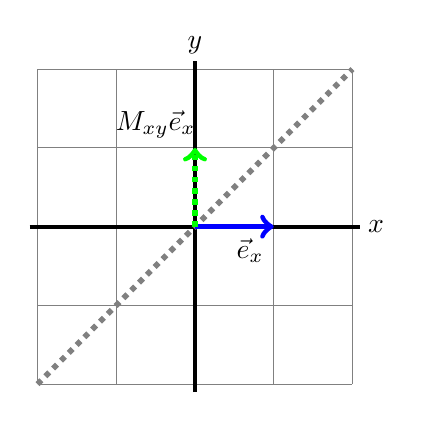
\begin{tikzpicture}
\draw[step=1.0,gray,thin] (-2,-2) grid (2,2);
\draw[black, line width=0.05 cm] (-2.1,0) -- (2.1,0);
\draw[black, line width=0.05 cm] (0,-2.1) -- (0,2.1);
\node at (0,2.3) {$y$};
\node at (2.3,0) {$x$};

\draw[gray, line width=0.07 cm, -,dotted] (-2,-2) -- (2,2);
\node at (0.7,-0.3) {$\vec{e}_x$};
\draw[blue, line width=0.07 cm,->] (0,0) -- (1,0);
\draw[green, line width=0.07 cm, ->,dotted] (0,0) -- (0,1);

\node at (-0.5,1.3) {$M_{xy} \vec{e}_x$};
\end{tikzpicture}
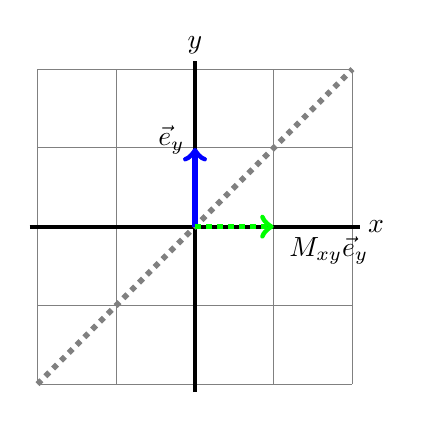
\begin{tikzpicture}
\draw[step=1.0,gray,thin] (-2,-2) grid (2,2);
\draw[black, line width=0.05 cm] (-2.1,0) -- (2.1,0);
\draw[black, line width=0.05 cm] (0,-2.1) -- (0,2.1);
\node at (0,2.3) {$y$};
\node at (2.3,0) {$x$};

\draw[gray, line width=0.07 cm, -,dotted] (-2,-2) -- (2,2);
\node at (-0.3,1.1) {$\vec{e}_y$};
\draw[blue, line width=0.07 cm,->] (0,0) -- (0,1);
\draw[green, line width=0.07 cm, ->,dotted] (0,0) -- (1,0);

\node at (1.7,-0.3) {$M_{xy} \vec{e}_y$};

\end{tikzpicture}
Now we know that:
\begin{equation*}
M_{xy}\vec{e}_x=\begin{pmatrix}0\\1\end{pmatrix}
\end{equation*}
And that:
\begin{equation*}
M_{xy}\vec{e}_y=\begin{pmatrix}1\\0\end{pmatrix}
\end{equation*}
These two vectors are the columns of our matrix and thus:
\begin{equation*}
M_{xy}=\begin{pmatrix}0&1\\1&0\end{pmatrix}
\end{equation*}
\Question Checking that the found eigenvectors and eigenvalues are indeed correct.\\
First we check$ \vec{v}_1$:
\begin{equation*}
M_{xy}\vec{v}_1=\begin{pmatrix}0&1\\1&0\end{pmatrix}\begin{pmatrix}1\\1\end{pmatrix}=\begin{pmatrix}1\\1\end{pmatrix}=1 \cdot \vec{v}_1
\end{equation*}
This is thus indeed an eigenvector of $M_{xy}$ with eigenvalue $1$. Now we proceed to check the same for $\vec{v}_2$:
\begin{equation*}
M_{xy}\vec{v}_2=\begin{pmatrix}0&1\\1&0\end{pmatrix}\begin{pmatrix}-1\\1\end{pmatrix}=\begin{pmatrix}1\\-1\end{pmatrix}=-1 \cdot \vec{v}_2
\end{equation*}
This is thus also an eigenvector. This eigenvector has eigenvalue $-1$.
\end{Answer}



\chapter{Solutions to the exercises}
\shipoutAnswer


\end{document}